\documentclass[twoside]{book}

% Packages required by doxygen
\usepackage{fixltx2e}
\usepackage{calc}
\usepackage{doxygen}
\usepackage[export]{adjustbox} % also loads graphicx
\usepackage{graphicx}
\usepackage[utf8]{inputenc}
\usepackage{makeidx}
\usepackage{multicol}
\usepackage{multirow}
\PassOptionsToPackage{warn}{textcomp}
\usepackage{textcomp}
\usepackage[nointegrals]{wasysym}
\usepackage[table]{xcolor}

% Font selection
\usepackage[T1]{fontenc}
\usepackage[scaled=.90]{helvet}
\usepackage{courier}
\usepackage{amssymb}
\usepackage{sectsty}
\renewcommand{\familydefault}{\sfdefault}
\allsectionsfont{%
  \fontseries{bc}\selectfont%
  \color{darkgray}%
}
\renewcommand{\DoxyLabelFont}{%
  \fontseries{bc}\selectfont%
  \color{darkgray}%
}
\newcommand{\+}{\discretionary{\mbox{\scriptsize$\hookleftarrow$}}{}{}}

% Page & text layout
\usepackage{geometry}
\geometry{%
  a4paper,%
  top=2.5cm,%
  bottom=2.5cm,%
  left=2.5cm,%
  right=2.5cm%
}
\tolerance=750
\hfuzz=15pt
\hbadness=750
\setlength{\emergencystretch}{15pt}
\setlength{\parindent}{0cm}
\setlength{\parskip}{3ex plus 2ex minus 2ex}
\makeatletter
\renewcommand{\paragraph}{%
  \@startsection{paragraph}{4}{0ex}{-1.0ex}{1.0ex}{%
    \normalfont\normalsize\bfseries\SS@parafont%
  }%
}
\renewcommand{\subparagraph}{%
  \@startsection{subparagraph}{5}{0ex}{-1.0ex}{1.0ex}{%
    \normalfont\normalsize\bfseries\SS@subparafont%
  }%
}
\makeatother

% Headers & footers
\usepackage{fancyhdr}
\pagestyle{fancyplain}
\fancyhead[LE]{\fancyplain{}{\bfseries\thepage}}
\fancyhead[CE]{\fancyplain{}{}}
\fancyhead[RE]{\fancyplain{}{\bfseries\leftmark}}
\fancyhead[LO]{\fancyplain{}{\bfseries\rightmark}}
\fancyhead[CO]{\fancyplain{}{}}
\fancyhead[RO]{\fancyplain{}{\bfseries\thepage}}
\fancyfoot[LE]{\fancyplain{}{}}
\fancyfoot[CE]{\fancyplain{}{}}
\fancyfoot[RE]{\fancyplain{}{\bfseries\scriptsize Generated by Doxygen }}
\fancyfoot[LO]{\fancyplain{}{\bfseries\scriptsize Generated by Doxygen }}
\fancyfoot[CO]{\fancyplain{}{}}
\fancyfoot[RO]{\fancyplain{}{}}
\renewcommand{\footrulewidth}{0.4pt}
\renewcommand{\chaptermark}[1]{%
  \markboth{#1}{}%
}
\renewcommand{\sectionmark}[1]{%
  \markright{\thesection\ #1}%
}

% Indices & bibliography
\usepackage{natbib}
\usepackage[titles]{tocloft}
\setcounter{tocdepth}{3}
\setcounter{secnumdepth}{5}
\makeindex

% Hyperlinks (required, but should be loaded last)
\usepackage{ifpdf}
\ifpdf
  \usepackage[pdftex,pagebackref=true]{hyperref}
\else
  \usepackage[ps2pdf,pagebackref=true]{hyperref}
\fi
\hypersetup{%
  colorlinks=true,%
  linkcolor=blue,%
  citecolor=blue,%
  unicode%
}

% Custom commands
\newcommand{\clearemptydoublepage}{%
  \newpage{\pagestyle{empty}\cleardoublepage}%
}

\usepackage{caption}
\captionsetup{labelsep=space,justification=centering,font={bf},singlelinecheck=off,skip=4pt,position=top}

%===== C O N T E N T S =====

\begin{document}

% Titlepage & ToC
\hypersetup{pageanchor=false,
             bookmarksnumbered=true,
             pdfencoding=unicode
            }
\pagenumbering{alph}
\begin{titlepage}
\vspace*{7cm}
\begin{center}%
{\Large R\+A\+I\+D5 }\\
\vspace*{1cm}
{\large Generated by Doxygen 1.8.13}\\
\end{center}
\end{titlepage}
\clearemptydoublepage
\pagenumbering{roman}
\tableofcontents
\clearemptydoublepage
\pagenumbering{arabic}
\hypersetup{pageanchor=true}

%--- Begin generated contents ---
\chapter{R\+A\+I\+D5}
\label{md__c_1_cygwin64_tmp__r_a_i_d5__r_e_a_d_m_e}
\Hypertarget{md__c_1_cygwin64_tmp__r_a_i_d5__r_e_a_d_m_e}
A final project for the Gvahim program. This project offers a system that can store your data on multiple servers, and back them up based on the R\+A\+I\+D5 protocol (Redundant Array of Independent Disks). The system lets you manage your servers, and works perfectly even with one faulty block device.

\subsection*{Getting Started}

These instructions will get you a copy of the project up and running on your local machine for development and testing purposes.

\subsubsection*{Prerequisites}

Here are the things you will need to download in order to get this system up and running\+:


\begin{DoxyCode}
1) Download and install Python2.7
2) Download this repository on your machine (Windows coming soon)
3) Download and install any modern browser
\end{DoxyCode}


\paragraph*{Browser Issues}

Chrome\+: By default, chrome doesn\textquotesingle{}t save form data upon refresh. Therefore on \char`\"{}\+Manage Disks\char`\"{}, the refresh time might not be sufficient for user purposes. Looking into solutions.

Firefox\+: Firefox currently disables basic authentication so could be problematical and will need to add this option manually. This can be done in the about\+:config section of firefox. Looking into better solutions

\subsubsection*{Execution}

Running the servers can be done as follows\+:

W\+I\+N\+D\+O\+WS \& L\+I\+N\+UX A\+L\+I\+KE\+:

Reach parent directory (R\+A\+I\+D5) 
\begin{DoxyCode}
cd [location of RAID5]
\end{DoxyCode}
 Running Frontend Server\+: 
\begin{DoxyCode}
python -m frontend [args]
\end{DoxyCode}
 Running Block Device Server\+: 
\begin{DoxyCode}
python -m block\_device [args]
\end{DoxyCode}


Testing the servers can be done from any browser. Basic Authentication is required with common\+\_\+user and common\+\_\+password specified in frontend/config.\+ini.

\subsubsection*{Arguments}

In both the Frontend and the Block Devices, the configuration file needs to be specified as args. The Block Devices also require a bind port as shown below\+: 
\begin{DoxyCode}
python -m frontend --config-file frontend/config.ini
python -m block\_device --config-file block\_device/disks/config0.ini --bind-port 8090
python -m block\_device --config-file block\_device/disks/config1.ini --bind-port 8091
\end{DoxyCode}
 Note\+: All other Arguments are optional, see --help for help

Note\+: Default configuration files are provided in this repository. The configuration files can be created from scratch (new U\+U\+I\+Ds and such) by a python script from the parent directory (R\+A\+I\+D5)\+: 
\begin{DoxyCode}
python config\_disks.py <NUM\_OF\_BLOCK\_DEVICES>
\end{DoxyCode}
 Note\+: U\+U\+ID\textquotesingle{}s can be changed manually from the configuration files

\subsubsection*{Testing}

Another python test script from the parent directory (R\+A\+I\+D5), has also been provided, that writes to the first disk (disk0) a long sequence of numbers, for testing purposes\+: 
\begin{DoxyCode}
python test.py
\end{DoxyCode}


\subsection*{Authors}


\begin{DoxyItemize}
\item {\bfseries Roy Zohar} -\/ {\itshape Initial work} -\/ \href{https://github.com/Royz2123}{\tt My Profile}
\end{DoxyItemize}

See also the list of \href{https://github.com/Royz2123/RAID5/contributors}{\tt contributors} who participated in this project.

\subsection*{Acknowledgments}


\begin{DoxyItemize}
\item A huge thanks to Alon and Sarit for all the support 
\end{DoxyItemize}
\chapter{Hierarchical Index}
\section{Class Hierarchy}
This inheritance list is sorted roughly, but not completely, alphabetically\+:\begin{DoxyCompactList}
\item Base\+Service\begin{DoxyCompactList}
\item \contentsline{section}{R\+A\+I\+D5.\+block\+\_\+device.\+services.\+get\+\_\+block\+\_\+service.\+Get\+Block\+Service}{\pageref{class_r_a_i_d5_1_1block__device_1_1services_1_1get__block__service_1_1_get_block_service}}{}
\item \contentsline{section}{R\+A\+I\+D5.\+block\+\_\+device.\+services.\+get\+\_\+disk\+\_\+info\+\_\+service.\+Get\+Disk\+Info\+Service}{\pageref{class_r_a_i_d5_1_1block__device_1_1services_1_1get__disk__info__service_1_1_get_disk_info_service}}{}
\item \contentsline{section}{R\+A\+I\+D5.\+block\+\_\+device.\+services.\+login\+\_\+service.\+Login\+Service}{\pageref{class_r_a_i_d5_1_1block__device_1_1services_1_1login__service_1_1_login_service}}{}
\item \contentsline{section}{R\+A\+I\+D5.\+block\+\_\+device.\+services.\+set\+\_\+block\+\_\+service.\+Set\+Block\+Service}{\pageref{class_r_a_i_d5_1_1block__device_1_1services_1_1set__block__service_1_1_set_block_service}}{}
\item \contentsline{section}{R\+A\+I\+D5.\+block\+\_\+device.\+services.\+set\+\_\+disk\+\_\+info\+\_\+service.\+Set\+Disk\+Info\+Service}{\pageref{class_r_a_i_d5_1_1block__device_1_1services_1_1set__disk__info__service_1_1_set_disk_info_service}}{}
\item \contentsline{section}{R\+A\+I\+D5.\+block\+\_\+device.\+services.\+update\+\_\+level\+\_\+service.\+Update\+Level\+Service}{\pageref{class_r_a_i_d5_1_1block__device_1_1services_1_1update__level__service_1_1_update_level_service}}{}
\item \contentsline{section}{R\+A\+I\+D5.\+frontend.\+services.\+client\+\_\+services.\+Client\+Service}{\pageref{class_r_a_i_d5_1_1frontend_1_1services_1_1client__services_1_1_client_service}}{}
\item \contentsline{section}{R\+A\+I\+D5.\+frontend.\+services.\+connect\+\_\+service.\+Connect\+Service}{\pageref{class_r_a_i_d5_1_1frontend_1_1services_1_1connect__service_1_1_connect_service}}{}
\item \contentsline{section}{R\+A\+I\+D5.\+frontend.\+services.\+disconnect\+\_\+service.\+Disconnect\+Service}{\pageref{class_r_a_i_d5_1_1frontend_1_1services_1_1disconnect__service_1_1_disconnect_service}}{}
\item \contentsline{section}{R\+A\+I\+D5.\+frontend.\+services.\+display\+\_\+disks\+\_\+service.\+Display\+Disks\+Service}{\pageref{class_r_a_i_d5_1_1frontend_1_1services_1_1display__disks__service_1_1_display_disks_service}}{}
\item \contentsline{section}{R\+A\+I\+D5.\+frontend.\+services.\+init\+\_\+service.\+Init\+Service}{\pageref{class_r_a_i_d5_1_1frontend_1_1services_1_1init__service_1_1_init_service}}{}
\item \contentsline{section}{R\+A\+I\+D5.\+frontend.\+services.\+management\+\_\+service.\+Management\+Service}{\pageref{class_r_a_i_d5_1_1frontend_1_1services_1_1management__service_1_1_management_service}}{}
\item \contentsline{section}{R\+A\+I\+D5.\+frontend.\+services.\+mul\+\_\+service.\+Mul\+Service}{\pageref{class_r_a_i_d5_1_1frontend_1_1services_1_1mul__service_1_1_mul_service}}{}
\item \contentsline{section}{R\+A\+I\+D5.\+frontend.\+services.\+read\+\_\+disk\+\_\+service.\+Read\+From\+Disk\+Service}{\pageref{class_r_a_i_d5_1_1frontend_1_1services_1_1read__disk__service_1_1_read_from_disk_service}}{}
\item \contentsline{section}{R\+A\+I\+D5.\+frontend.\+services.\+time\+\_\+service.\+Time\+Service}{\pageref{class_r_a_i_d5_1_1frontend_1_1services_1_1time__service_1_1_time_service}}{}
\item \contentsline{section}{R\+A\+I\+D5.\+frontend.\+services.\+write\+\_\+disk\+\_\+service.\+Write\+To\+Disk\+Service}{\pageref{class_r_a_i_d5_1_1frontend_1_1services_1_1write__disk__service_1_1_write_to_disk_service}}{}
\end{DoxyCompactList}
\item File\+Form\+Service\begin{DoxyCompactList}
\item \contentsline{section}{R\+A\+I\+D5.\+block\+\_\+device.\+services.\+set\+\_\+disk\+\_\+info\+\_\+service.\+Set\+Disk\+Info\+Service}{\pageref{class_r_a_i_d5_1_1block__device_1_1services_1_1set__disk__info__service_1_1_set_disk_info_service}}{}
\item \contentsline{section}{R\+A\+I\+D5.\+frontend.\+services.\+write\+\_\+disk\+\_\+service.\+Write\+To\+Disk\+Service}{\pageref{class_r_a_i_d5_1_1frontend_1_1services_1_1write__disk__service_1_1_write_to_disk_service}}{}
\end{DoxyCompactList}
\item Get\+File\+Service\begin{DoxyCompactList}
\item \contentsline{section}{R\+A\+I\+D5.\+block\+\_\+device.\+services.\+get\+\_\+disk\+\_\+info\+\_\+service.\+Get\+Disk\+Info\+Service}{\pageref{class_r_a_i_d5_1_1block__device_1_1services_1_1get__disk__info__service_1_1_get_disk_info_service}}{}
\end{DoxyCompactList}
\item object\begin{DoxyCompactList}
\item \contentsline{section}{R\+A\+I\+D5.\+common.\+pollables.\+callable.\+Callable}{\pageref{class_r_a_i_d5_1_1common_1_1pollables_1_1callable_1_1_callable}}{}
\begin{DoxyCompactList}
\item \contentsline{section}{R\+A\+I\+D5.\+common.\+pollables.\+service\+\_\+socket.\+Service\+Socket}{\pageref{class_r_a_i_d5_1_1common_1_1pollables_1_1service__socket_1_1_service_socket}}{}
\end{DoxyCompactList}
\item \contentsline{section}{R\+A\+I\+D5.\+common.\+pollables.\+pollable.\+Pollable}{\pageref{class_r_a_i_d5_1_1common_1_1pollables_1_1pollable_1_1_pollable}}{}
\begin{DoxyCompactList}
\item \contentsline{section}{R\+A\+I\+D5.\+common.\+pollables.\+listener\+\_\+socket.\+Listener\+Socket}{\pageref{class_r_a_i_d5_1_1common_1_1pollables_1_1listener__socket_1_1_listener_socket}}{}
\item \contentsline{section}{R\+A\+I\+D5.\+common.\+pollables.\+service\+\_\+socket.\+Service\+Socket}{\pageref{class_r_a_i_d5_1_1common_1_1pollables_1_1service__socket_1_1_service_socket}}{}
\end{DoxyCompactList}
\item \contentsline{section}{R\+A\+I\+D5.\+common.\+services.\+base\+\_\+service.\+Base\+Service}{\pageref{class_r_a_i_d5_1_1common_1_1services_1_1base__service_1_1_base_service}}{}
\begin{DoxyCompactList}
\item \contentsline{section}{R\+A\+I\+D5.\+common.\+services.\+form\+\_\+service.\+File\+Form\+Service}{\pageref{class_r_a_i_d5_1_1common_1_1services_1_1form__service_1_1_file_form_service}}{}
\item \contentsline{section}{R\+A\+I\+D5.\+common.\+services.\+get\+\_\+file\+\_\+service.\+Get\+File\+Service}{\pageref{class_r_a_i_d5_1_1common_1_1services_1_1get__file__service_1_1_get_file_service}}{}
\end{DoxyCompactList}
\item \contentsline{section}{R\+A\+I\+D5.\+common.\+utilities.\+async\+\_\+server.\+Async\+Server}{\pageref{class_r_a_i_d5_1_1common_1_1utilities_1_1async__server_1_1_async_server}}{}
\item \contentsline{section}{R\+A\+I\+D5.\+common.\+utilities.\+state\+\_\+util.\+state.\+State}{\pageref{class_r_a_i_d5_1_1common_1_1utilities_1_1state__util_1_1state_1_1_state}}{}
\item \contentsline{section}{R\+A\+I\+D5.\+common.\+utilities.\+state\+\_\+util.\+state\+\_\+machine.\+State\+Machine}{\pageref{class_r_a_i_d5_1_1common_1_1utilities_1_1state__util_1_1state__machine_1_1_state_machine}}{}
\item \contentsline{section}{R\+A\+I\+D5.\+frontend.\+utilities.\+cache.\+Cache}{\pageref{class_r_a_i_d5_1_1frontend_1_1utilities_1_1cache_1_1_cache}}{}
\item \contentsline{section}{R\+A\+I\+D5.\+frontend.\+utilities.\+disk\+\_\+manager.\+Disk\+Manager}{\pageref{class_r_a_i_d5_1_1frontend_1_1utilities_1_1disk__manager_1_1_disk_manager}}{}
\item \contentsline{section}{state.\+State}{\pageref{classstate_1_1_state}}{}
\item \contentsline{section}{state\+\_\+machine.\+State\+Machine}{\pageref{classstate__machine_1_1_state_machine}}{}
\end{DoxyCompactList}
\item Pollable\begin{DoxyCompactList}
\item \contentsline{section}{R\+A\+I\+D5.\+block\+\_\+device.\+pollables.\+declarer\+\_\+socket.\+Declarer\+Socket}{\pageref{class_r_a_i_d5_1_1block__device_1_1pollables_1_1declarer__socket_1_1_declarer_socket}}{}
\item \contentsline{section}{R\+A\+I\+D5.\+frontend.\+pollables.\+bds\+\_\+client\+\_\+socket.\+B\+D\+S\+Client\+Socket}{\pageref{class_r_a_i_d5_1_1frontend_1_1pollables_1_1bds__client__socket_1_1_b_d_s_client_socket}}{}
\item \contentsline{section}{R\+A\+I\+D5.\+frontend.\+pollables.\+identifier\+\_\+socket.\+Identifier\+Socket}{\pageref{class_r_a_i_d5_1_1frontend_1_1pollables_1_1identifier__socket_1_1_identifier_socket}}{}
\end{DoxyCompactList}
\item \contentsline{section}{R\+A\+I\+D5.\+common.\+utilities.\+poller.\+Poller}{\pageref{class_r_a_i_d5_1_1common_1_1utilities_1_1poller_1_1_poller}}{}
\item Runtime\+Error\begin{DoxyCompactList}
\item \contentsline{section}{R\+A\+I\+D5.\+common.\+utilities.\+util.\+Disconnect}{\pageref{class_r_a_i_d5_1_1common_1_1utilities_1_1util_1_1_disconnect}}{}
\item \contentsline{section}{R\+A\+I\+D5.\+common.\+utilities.\+util.\+Disk\+Refused}{\pageref{class_r_a_i_d5_1_1common_1_1utilities_1_1util_1_1_disk_refused}}{}
\item \contentsline{section}{R\+A\+I\+D5.\+common.\+utilities.\+util.\+Invalid\+Arguments}{\pageref{class_r_a_i_d5_1_1common_1_1utilities_1_1util_1_1_invalid_arguments}}{}
\end{DoxyCompactList}
\item \contentsline{section}{R\+A\+I\+D5.\+common.\+utilities.\+poller.\+Select}{\pageref{class_r_a_i_d5_1_1common_1_1utilities_1_1poller_1_1_select}}{}
\end{DoxyCompactList}

\chapter{Class Index}
\section{Class List}
Here are the classes, structs, unions and interfaces with brief descriptions\+:\begin{DoxyCompactList}
\item\contentsline{section}{\hyperlink{class_r_a_i_d5_1_1common_1_1utilities_1_1async__server_1_1_async_server}{R\+A\+I\+D5.\+common.\+utilities.\+async\+\_\+server.\+Async\+Server} }{\pageref{class_r_a_i_d5_1_1common_1_1utilities_1_1async__server_1_1_async_server}}{}
\item\contentsline{section}{\hyperlink{class_r_a_i_d5_1_1common_1_1services_1_1base__service_1_1_base_service}{R\+A\+I\+D5.\+common.\+services.\+base\+\_\+service.\+Base\+Service} }{\pageref{class_r_a_i_d5_1_1common_1_1services_1_1base__service_1_1_base_service}}{}
\item\contentsline{section}{\hyperlink{class_r_a_i_d5_1_1frontend_1_1pollables_1_1bds__client__socket_1_1_b_d_s_client_socket}{R\+A\+I\+D5.\+frontend.\+pollables.\+bds\+\_\+client\+\_\+socket.\+B\+D\+S\+Client\+Socket} }{\pageref{class_r_a_i_d5_1_1frontend_1_1pollables_1_1bds__client__socket_1_1_b_d_s_client_socket}}{}
\item\contentsline{section}{\hyperlink{class_r_a_i_d5_1_1frontend_1_1utilities_1_1cache_1_1_cache}{R\+A\+I\+D5.\+frontend.\+utilities.\+cache.\+Cache} }{\pageref{class_r_a_i_d5_1_1frontend_1_1utilities_1_1cache_1_1_cache}}{}
\item\contentsline{section}{\hyperlink{class_r_a_i_d5_1_1common_1_1pollables_1_1callable_1_1_callable}{R\+A\+I\+D5.\+common.\+pollables.\+callable.\+Callable} }{\pageref{class_r_a_i_d5_1_1common_1_1pollables_1_1callable_1_1_callable}}{}
\item\contentsline{section}{\hyperlink{class_r_a_i_d5_1_1frontend_1_1services_1_1client__services_1_1_client_service}{R\+A\+I\+D5.\+frontend.\+services.\+client\+\_\+services.\+Client\+Service} }{\pageref{class_r_a_i_d5_1_1frontend_1_1services_1_1client__services_1_1_client_service}}{}
\item\contentsline{section}{\hyperlink{class_r_a_i_d5_1_1frontend_1_1services_1_1connect__service_1_1_connect_service}{R\+A\+I\+D5.\+frontend.\+services.\+connect\+\_\+service.\+Connect\+Service} }{\pageref{class_r_a_i_d5_1_1frontend_1_1services_1_1connect__service_1_1_connect_service}}{}
\item\contentsline{section}{\hyperlink{class_r_a_i_d5_1_1block__device_1_1pollables_1_1declarer__socket_1_1_declarer_socket}{R\+A\+I\+D5.\+block\+\_\+device.\+pollables.\+declarer\+\_\+socket.\+Declarer\+Socket} \\*A Block Device Socket that declares the server using U\+DP Multicast to other Frontend Servers to recognize }{\pageref{class_r_a_i_d5_1_1block__device_1_1pollables_1_1declarer__socket_1_1_declarer_socket}}{}
\item\contentsline{section}{\hyperlink{class_r_a_i_d5_1_1common_1_1utilities_1_1util_1_1_disconnect}{R\+A\+I\+D5.\+common.\+utilities.\+util.\+Disconnect} }{\pageref{class_r_a_i_d5_1_1common_1_1utilities_1_1util_1_1_disconnect}}{}
\item\contentsline{section}{\hyperlink{class_r_a_i_d5_1_1frontend_1_1services_1_1disconnect__service_1_1_disconnect_service}{R\+A\+I\+D5.\+frontend.\+services.\+disconnect\+\_\+service.\+Disconnect\+Service} }{\pageref{class_r_a_i_d5_1_1frontend_1_1services_1_1disconnect__service_1_1_disconnect_service}}{}
\item\contentsline{section}{\hyperlink{class_r_a_i_d5_1_1frontend_1_1utilities_1_1disk__manager_1_1_disk_manager}{R\+A\+I\+D5.\+frontend.\+utilities.\+disk\+\_\+manager.\+Disk\+Manager} }{\pageref{class_r_a_i_d5_1_1frontend_1_1utilities_1_1disk__manager_1_1_disk_manager}}{}
\item\contentsline{section}{\hyperlink{class_r_a_i_d5_1_1common_1_1utilities_1_1util_1_1_disk_refused}{R\+A\+I\+D5.\+common.\+utilities.\+util.\+Disk\+Refused} }{\pageref{class_r_a_i_d5_1_1common_1_1utilities_1_1util_1_1_disk_refused}}{}
\item\contentsline{section}{\hyperlink{class_r_a_i_d5_1_1frontend_1_1services_1_1display__disks__service_1_1_display_disks_service}{R\+A\+I\+D5.\+frontend.\+services.\+display\+\_\+disks\+\_\+service.\+Display\+Disks\+Service} }{\pageref{class_r_a_i_d5_1_1frontend_1_1services_1_1display__disks__service_1_1_display_disks_service}}{}
\item\contentsline{section}{\hyperlink{class_r_a_i_d5_1_1common_1_1services_1_1form__service_1_1_file_form_service}{R\+A\+I\+D5.\+common.\+services.\+form\+\_\+service.\+File\+Form\+Service} }{\pageref{class_r_a_i_d5_1_1common_1_1services_1_1form__service_1_1_file_form_service}}{}
\item\contentsline{section}{\hyperlink{class_r_a_i_d5_1_1block__device_1_1services_1_1get__block__service_1_1_get_block_service}{R\+A\+I\+D5.\+block\+\_\+device.\+services.\+get\+\_\+block\+\_\+service.\+Get\+Block\+Service} \\*A Block Device Service that allows the Frontend Server to request a block }{\pageref{class_r_a_i_d5_1_1block__device_1_1services_1_1get__block__service_1_1_get_block_service}}{}
\item\contentsline{section}{\hyperlink{class_r_a_i_d5_1_1block__device_1_1services_1_1get__disk__info__service_1_1_get_disk_info_service}{R\+A\+I\+D5.\+block\+\_\+device.\+services.\+get\+\_\+disk\+\_\+info\+\_\+service.\+Get\+Disk\+Info\+Service} \\*A Block Device Service that sends the Frontend it\textquotesingle{}s disk info (block -\/1) Very simple class, just sets the disk\+\_\+info location and then regular \hyperlink{class_r_a_i_d5_1_1common_1_1services_1_1get__file__service_1_1_get_file_service}{common.\+services.\+get\+\_\+file\+\_\+service.\+Get\+File\+Service} }{\pageref{class_r_a_i_d5_1_1block__device_1_1services_1_1get__disk__info__service_1_1_get_disk_info_service}}{}
\item\contentsline{section}{\hyperlink{class_r_a_i_d5_1_1common_1_1services_1_1get__file__service_1_1_get_file_service}{R\+A\+I\+D5.\+common.\+services.\+get\+\_\+file\+\_\+service.\+Get\+File\+Service} }{\pageref{class_r_a_i_d5_1_1common_1_1services_1_1get__file__service_1_1_get_file_service}}{}
\item\contentsline{section}{\hyperlink{class_r_a_i_d5_1_1frontend_1_1pollables_1_1identifier__socket_1_1_identifier_socket}{R\+A\+I\+D5.\+frontend.\+pollables.\+identifier\+\_\+socket.\+Identifier\+Socket} }{\pageref{class_r_a_i_d5_1_1frontend_1_1pollables_1_1identifier__socket_1_1_identifier_socket}}{}
\item\contentsline{section}{\hyperlink{class_r_a_i_d5_1_1frontend_1_1services_1_1init__service_1_1_init_service}{R\+A\+I\+D5.\+frontend.\+services.\+init\+\_\+service.\+Init\+Service} }{\pageref{class_r_a_i_d5_1_1frontend_1_1services_1_1init__service_1_1_init_service}}{}
\item\contentsline{section}{\hyperlink{class_r_a_i_d5_1_1common_1_1utilities_1_1util_1_1_invalid_arguments}{R\+A\+I\+D5.\+common.\+utilities.\+util.\+Invalid\+Arguments} }{\pageref{class_r_a_i_d5_1_1common_1_1utilities_1_1util_1_1_invalid_arguments}}{}
\item\contentsline{section}{\hyperlink{class_r_a_i_d5_1_1common_1_1pollables_1_1listener__socket_1_1_listener_socket}{R\+A\+I\+D5.\+common.\+pollables.\+listener\+\_\+socket.\+Listener\+Socket} }{\pageref{class_r_a_i_d5_1_1common_1_1pollables_1_1listener__socket_1_1_listener_socket}}{}
\item\contentsline{section}{\hyperlink{class_r_a_i_d5_1_1block__device_1_1services_1_1login__service_1_1_login_service}{R\+A\+I\+D5.\+block\+\_\+device.\+services.\+login\+\_\+service.\+Login\+Service} \\*A Block Device Service that allows the Frontend to supply it with a long\+\_\+password for later communication }{\pageref{class_r_a_i_d5_1_1block__device_1_1services_1_1login__service_1_1_login_service}}{}
\item\contentsline{section}{\hyperlink{class_r_a_i_d5_1_1frontend_1_1services_1_1management__service_1_1_management_service}{R\+A\+I\+D5.\+frontend.\+services.\+management\+\_\+service.\+Management\+Service} }{\pageref{class_r_a_i_d5_1_1frontend_1_1services_1_1management__service_1_1_management_service}}{}
\item\contentsline{section}{\hyperlink{class_r_a_i_d5_1_1frontend_1_1services_1_1mul__service_1_1_mul_service}{R\+A\+I\+D5.\+frontend.\+services.\+mul\+\_\+service.\+Mul\+Service} }{\pageref{class_r_a_i_d5_1_1frontend_1_1services_1_1mul__service_1_1_mul_service}}{}
\item\contentsline{section}{\hyperlink{class_r_a_i_d5_1_1common_1_1pollables_1_1pollable_1_1_pollable}{R\+A\+I\+D5.\+common.\+pollables.\+pollable.\+Pollable} }{\pageref{class_r_a_i_d5_1_1common_1_1pollables_1_1pollable_1_1_pollable}}{}
\item\contentsline{section}{\hyperlink{class_r_a_i_d5_1_1common_1_1utilities_1_1poller_1_1_poller}{R\+A\+I\+D5.\+common.\+utilities.\+poller.\+Poller} }{\pageref{class_r_a_i_d5_1_1common_1_1utilities_1_1poller_1_1_poller}}{}
\item\contentsline{section}{\hyperlink{class_r_a_i_d5_1_1frontend_1_1services_1_1read__disk__service_1_1_read_from_disk_service}{R\+A\+I\+D5.\+frontend.\+services.\+read\+\_\+disk\+\_\+service.\+Read\+From\+Disk\+Service} }{\pageref{class_r_a_i_d5_1_1frontend_1_1services_1_1read__disk__service_1_1_read_from_disk_service}}{}
\item\contentsline{section}{\hyperlink{class_r_a_i_d5_1_1common_1_1utilities_1_1poller_1_1_select}{R\+A\+I\+D5.\+common.\+utilities.\+poller.\+Select} }{\pageref{class_r_a_i_d5_1_1common_1_1utilities_1_1poller_1_1_select}}{}
\item\contentsline{section}{\hyperlink{class_r_a_i_d5_1_1common_1_1pollables_1_1service__socket_1_1_service_socket}{R\+A\+I\+D5.\+common.\+pollables.\+service\+\_\+socket.\+Service\+Socket} }{\pageref{class_r_a_i_d5_1_1common_1_1pollables_1_1service__socket_1_1_service_socket}}{}
\item\contentsline{section}{\hyperlink{class_r_a_i_d5_1_1block__device_1_1services_1_1set__block__service_1_1_set_block_service}{R\+A\+I\+D5.\+block\+\_\+device.\+services.\+set\+\_\+block\+\_\+service.\+Set\+Block\+Service} \\*A Block Device Service that allows the Frontend Server to set a block }{\pageref{class_r_a_i_d5_1_1block__device_1_1services_1_1set__block__service_1_1_set_block_service}}{}
\item\contentsline{section}{\hyperlink{class_r_a_i_d5_1_1block__device_1_1services_1_1set__disk__info__service_1_1_set_disk_info_service}{R\+A\+I\+D5.\+block\+\_\+device.\+services.\+set\+\_\+disk\+\_\+info\+\_\+service.\+Set\+Disk\+Info\+Service} \\*A Block Device Service that modifies it\textquotesingle{}s disk info (block -\/1) Very simple class, just sets the disk\+\_\+info location and then regular \hyperlink{class_r_a_i_d5_1_1common_1_1services_1_1form__service_1_1_file_form_service}{common.\+services.\+form\+\_\+service.\+File\+Form\+Service} }{\pageref{class_r_a_i_d5_1_1block__device_1_1services_1_1set__disk__info__service_1_1_set_disk_info_service}}{}
\item\contentsline{section}{\hyperlink{classstate_1_1_state}{state.\+State} }{\pageref{classstate_1_1_state}}{}
\item\contentsline{section}{\hyperlink{class_r_a_i_d5_1_1common_1_1utilities_1_1state__util_1_1state_1_1_state}{R\+A\+I\+D5.\+common.\+utilities.\+state\+\_\+util.\+state.\+State} }{\pageref{class_r_a_i_d5_1_1common_1_1utilities_1_1state__util_1_1state_1_1_state}}{}
\item\contentsline{section}{\hyperlink{classstate__machine_1_1_state_machine}{state\+\_\+machine.\+State\+Machine} }{\pageref{classstate__machine_1_1_state_machine}}{}
\item\contentsline{section}{\hyperlink{class_r_a_i_d5_1_1common_1_1utilities_1_1state__util_1_1state__machine_1_1_state_machine}{R\+A\+I\+D5.\+common.\+utilities.\+state\+\_\+util.\+state\+\_\+machine.\+State\+Machine} }{\pageref{class_r_a_i_d5_1_1common_1_1utilities_1_1state__util_1_1state__machine_1_1_state_machine}}{}
\item\contentsline{section}{\hyperlink{class_r_a_i_d5_1_1frontend_1_1services_1_1time__service_1_1_time_service}{R\+A\+I\+D5.\+frontend.\+services.\+time\+\_\+service.\+Time\+Service} }{\pageref{class_r_a_i_d5_1_1frontend_1_1services_1_1time__service_1_1_time_service}}{}
\item\contentsline{section}{\hyperlink{class_r_a_i_d5_1_1block__device_1_1services_1_1update__level__service_1_1_update_level_service}{R\+A\+I\+D5.\+block\+\_\+device.\+services.\+update\+\_\+level\+\_\+service.\+Update\+Level\+Service} \\*A Block Device Service that updates the level of the disk\+\_\+info file Also known as generation id Created in order to simplify the handling of the disk info file, and to save unnecessary calls the block device services\+: \hyperlink{class_r_a_i_d5_1_1block__device_1_1services_1_1get__disk__info__service_1_1_get_disk_info_service}{block\+\_\+device.\+services.\+get\+\_\+disk\+\_\+info\+\_\+service.\+Get\+Disk\+Info\+Service} and \hyperlink{class_r_a_i_d5_1_1block__device_1_1services_1_1set__disk__info__service_1_1_set_disk_info_service}{block\+\_\+device.\+services.\+set\+\_\+disk\+\_\+info\+\_\+service.\+Set\+Disk\+Info\+Service} }{\pageref{class_r_a_i_d5_1_1block__device_1_1services_1_1update__level__service_1_1_update_level_service}}{}
\item\contentsline{section}{\hyperlink{class_r_a_i_d5_1_1frontend_1_1services_1_1write__disk__service_1_1_write_to_disk_service}{R\+A\+I\+D5.\+frontend.\+services.\+write\+\_\+disk\+\_\+service.\+Write\+To\+Disk\+Service} }{\pageref{class_r_a_i_d5_1_1frontend_1_1services_1_1write__disk__service_1_1_write_to_disk_service}}{}
\end{DoxyCompactList}

\chapter{Class Documentation}
\hypertarget{class_r_a_i_d5_1_1common_1_1utilities_1_1async__server_1_1_async_server}{}\section{R\+A\+I\+D5.\+common.\+utilities.\+async\+\_\+server.\+Async\+Server Class Reference}
\label{class_r_a_i_d5_1_1common_1_1utilities_1_1async__server_1_1_async_server}\index{R\+A\+I\+D5.\+common.\+utilities.\+async\+\_\+server.\+Async\+Server@{R\+A\+I\+D5.\+common.\+utilities.\+async\+\_\+server.\+Async\+Server}}
Inheritance diagram for R\+A\+I\+D5.\+common.\+utilities.\+async\+\_\+server.\+Async\+Server\+:\begin{figure}[H]
\begin{center}
\leavevmode
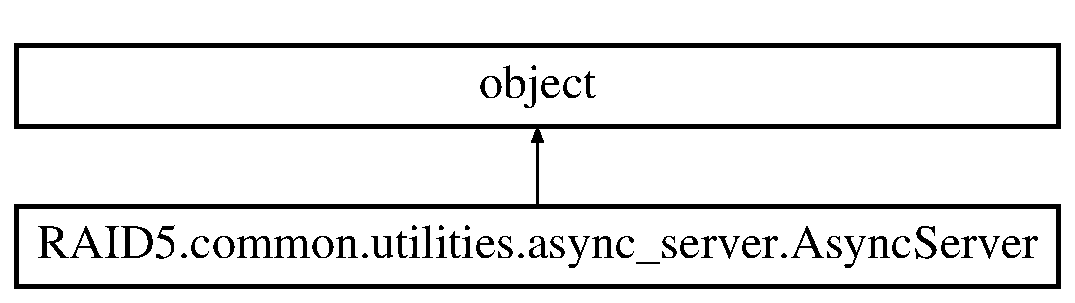
\includegraphics[height=2.000000cm]{class_r_a_i_d5_1_1common_1_1utilities_1_1async__server_1_1_async_server}
\end{center}
\end{figure}
\subsection*{Public Member Functions}
\begin{DoxyCompactItemize}
\item 
\mbox{\Hypertarget{class_r_a_i_d5_1_1common_1_1utilities_1_1async__server_1_1_async_server_af174e7bc529ce4d05bd2883a9af50281}\label{class_r_a_i_d5_1_1common_1_1utilities_1_1async__server_1_1_async_server_af174e7bc529ce4d05bd2883a9af50281}} 
def {\bfseries \+\_\+\+\_\+init\+\_\+\+\_\+} (self, application\+\_\+context)
\item 
\mbox{\Hypertarget{class_r_a_i_d5_1_1common_1_1utilities_1_1async__server_1_1_async_server_a6391f488e2292a508b0688ac15e1c9fc}\label{class_r_a_i_d5_1_1common_1_1utilities_1_1async__server_1_1_async_server_a6391f488e2292a508b0688ac15e1c9fc}} 
def {\bfseries add\+\_\+listener} (self)
\item 
\mbox{\Hypertarget{class_r_a_i_d5_1_1common_1_1utilities_1_1async__server_1_1_async_server_a03c6d031cc16a3c916c81c6d50ed6594}\label{class_r_a_i_d5_1_1common_1_1utilities_1_1async__server_1_1_async_server_a03c6d031cc16a3c916c81c6d50ed6594}} 
def {\bfseries add\+\_\+declarer} (self)
\item 
\mbox{\Hypertarget{class_r_a_i_d5_1_1common_1_1utilities_1_1async__server_1_1_async_server_a1c5753ca0a100acadbabd90c55f620cf}\label{class_r_a_i_d5_1_1common_1_1utilities_1_1async__server_1_1_async_server_a1c5753ca0a100acadbabd90c55f620cf}} 
def {\bfseries add\+\_\+identifier} (self)
\item 
\mbox{\Hypertarget{class_r_a_i_d5_1_1common_1_1utilities_1_1async__server_1_1_async_server_aab3c4124e5e22f5c74228218e881aff4}\label{class_r_a_i_d5_1_1common_1_1utilities_1_1async__server_1_1_async_server_aab3c4124e5e22f5c74228218e881aff4}} 
def {\bfseries on\+\_\+start} (self)
\item 
\mbox{\Hypertarget{class_r_a_i_d5_1_1common_1_1utilities_1_1async__server_1_1_async_server_af8c460707920c3f1da35b8c0b5035987}\label{class_r_a_i_d5_1_1common_1_1utilities_1_1async__server_1_1_async_server_af8c460707920c3f1da35b8c0b5035987}} 
def {\bfseries handle\+\_\+events} (self, events)
\item 
\mbox{\Hypertarget{class_r_a_i_d5_1_1common_1_1utilities_1_1async__server_1_1_async_server_a712466f681b0e859825d9b83550a6892}\label{class_r_a_i_d5_1_1common_1_1utilities_1_1async__server_1_1_async_server_a712466f681b0e859825d9b83550a6892}} 
def {\bfseries timeout\+\_\+event} (self)
\item 
\mbox{\Hypertarget{class_r_a_i_d5_1_1common_1_1utilities_1_1async__server_1_1_async_server_a9ddc117230bb5e2cadedebe17eaff2aa}\label{class_r_a_i_d5_1_1common_1_1utilities_1_1async__server_1_1_async_server_a9ddc117230bb5e2cadedebe17eaff2aa}} 
def {\bfseries run} (self)
\item 
\mbox{\Hypertarget{class_r_a_i_d5_1_1common_1_1utilities_1_1async__server_1_1_async_server_ab7154ace3700577c788fcc079735e505}\label{class_r_a_i_d5_1_1common_1_1utilities_1_1async__server_1_1_async_server_ab7154ace3700577c788fcc079735e505}} 
def {\bfseries create\+\_\+poller} (self)
\item 
\mbox{\Hypertarget{class_r_a_i_d5_1_1common_1_1utilities_1_1async__server_1_1_async_server_aa4f6e6ce14625b565207c22554244097}\label{class_r_a_i_d5_1_1common_1_1utilities_1_1async__server_1_1_async_server_aa4f6e6ce14625b565207c22554244097}} 
def {\bfseries pollables} (self)
\item 
\mbox{\Hypertarget{class_r_a_i_d5_1_1common_1_1utilities_1_1async__server_1_1_async_server_a03fc561aa7bf92660cf926edc431e1f9}\label{class_r_a_i_d5_1_1common_1_1utilities_1_1async__server_1_1_async_server_a03fc561aa7bf92660cf926edc431e1f9}} 
def {\bfseries pollables} (self, s)
\item 
\mbox{\Hypertarget{class_r_a_i_d5_1_1common_1_1utilities_1_1async__server_1_1_async_server_afc6026c2e79b2ade1cc960c204a2bcb1}\label{class_r_a_i_d5_1_1common_1_1utilities_1_1async__server_1_1_async_server_afc6026c2e79b2ade1cc960c204a2bcb1}} 
def {\bfseries close\+\_\+needed} (self)
\item 
\mbox{\Hypertarget{class_r_a_i_d5_1_1common_1_1utilities_1_1async__server_1_1_async_server_a3ee5a7b99c9a7318817e2e2ebf6a7efb}\label{class_r_a_i_d5_1_1common_1_1utilities_1_1async__server_1_1_async_server_a3ee5a7b99c9a7318817e2e2ebf6a7efb}} 
def {\bfseries close\+\_\+all} (self)
\end{DoxyCompactItemize}


The documentation for this class was generated from the following file\+:\begin{DoxyCompactItemize}
\item 
C\+:/cygwin64/tmp/\+R\+A\+I\+D5/common/utilities/async\+\_\+server.\+py\end{DoxyCompactItemize}

\hypertarget{class_r_a_i_d5_1_1common_1_1services_1_1base__service_1_1_base_service}{}\section{R\+A\+I\+D5.\+common.\+services.\+base\+\_\+service.\+Base\+Service Class Reference}
\label{class_r_a_i_d5_1_1common_1_1services_1_1base__service_1_1_base_service}\index{R\+A\+I\+D5.\+common.\+services.\+base\+\_\+service.\+Base\+Service@{R\+A\+I\+D5.\+common.\+services.\+base\+\_\+service.\+Base\+Service}}
Inheritance diagram for R\+A\+I\+D5.\+common.\+services.\+base\+\_\+service.\+Base\+Service\+:\begin{figure}[H]
\begin{center}
\leavevmode
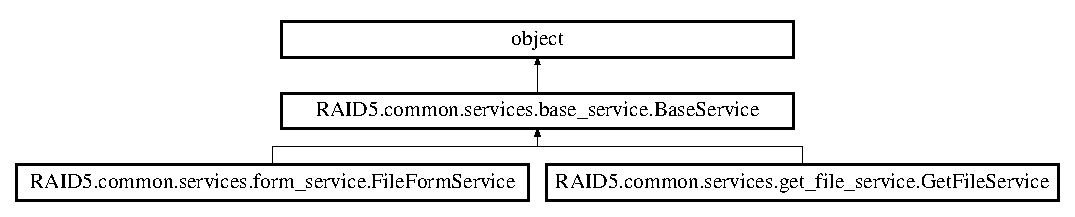
\includegraphics[height=2.470588cm]{class_r_a_i_d5_1_1common_1_1services_1_1base__service_1_1_base_service}
\end{center}
\end{figure}
\subsection*{Public Member Functions}
\begin{DoxyCompactItemize}
\item 
\mbox{\Hypertarget{class_r_a_i_d5_1_1common_1_1services_1_1base__service_1_1_base_service_a82d70b601ced4d8a265ad9c2895d1321}\label{class_r_a_i_d5_1_1common_1_1services_1_1base__service_1_1_base_service_a82d70b601ced4d8a265ad9c2895d1321}} 
def {\bfseries \+\_\+\+\_\+init\+\_\+\+\_\+} (self, wanted\+\_\+headers=\mbox{[}$\,$\mbox{]}, wanted\+\_\+args=\mbox{[}$\,$\mbox{]}, args=\{\})
\item 
\mbox{\Hypertarget{class_r_a_i_d5_1_1common_1_1services_1_1base__service_1_1_base_service_aa52ac7f28702d461220e448726f39c54}\label{class_r_a_i_d5_1_1common_1_1services_1_1base__service_1_1_base_service_aa52ac7f28702d461220e448726f39c54}} 
def {\bfseries args} (self)
\item 
\mbox{\Hypertarget{class_r_a_i_d5_1_1common_1_1services_1_1base__service_1_1_base_service_a7f5af0d2a6986026aea8a69f71934f8f}\label{class_r_a_i_d5_1_1common_1_1services_1_1base__service_1_1_base_service_a7f5af0d2a6986026aea8a69f71934f8f}} 
def {\bfseries args} (self, a)
\item 
\mbox{\Hypertarget{class_r_a_i_d5_1_1common_1_1services_1_1base__service_1_1_base_service_a152e00847b5be2beb3cdaa19fd1f7286}\label{class_r_a_i_d5_1_1common_1_1services_1_1base__service_1_1_base_service_a152e00847b5be2beb3cdaa19fd1f7286}} 
def {\bfseries wanted\+\_\+headers} (self)
\item 
\mbox{\Hypertarget{class_r_a_i_d5_1_1common_1_1services_1_1base__service_1_1_base_service_afcc19960fd34594a84b1ca4e17523adc}\label{class_r_a_i_d5_1_1common_1_1services_1_1base__service_1_1_base_service_afcc19960fd34594a84b1ca4e17523adc}} 
def {\bfseries wanted\+\_\+headers} (self, w\+\_\+h)
\item 
\mbox{\Hypertarget{class_r_a_i_d5_1_1common_1_1services_1_1base__service_1_1_base_service_a40a554ce7aaf51a959ab4083305635df}\label{class_r_a_i_d5_1_1common_1_1services_1_1base__service_1_1_base_service_a40a554ce7aaf51a959ab4083305635df}} 
def {\bfseries wanted\+\_\+args} (self)
\item 
\mbox{\Hypertarget{class_r_a_i_d5_1_1common_1_1services_1_1base__service_1_1_base_service_a4248500b960b9db631452d256fe4ed6d}\label{class_r_a_i_d5_1_1common_1_1services_1_1base__service_1_1_base_service_a4248500b960b9db631452d256fe4ed6d}} 
def {\bfseries wanted\+\_\+args} (self, w\+\_\+a)
\item 
\mbox{\Hypertarget{class_r_a_i_d5_1_1common_1_1services_1_1base__service_1_1_base_service_aa906012f9802c7158585d5ee028c3a89}\label{class_r_a_i_d5_1_1common_1_1services_1_1base__service_1_1_base_service_aa906012f9802c7158585d5ee028c3a89}} 
def {\bfseries response\+\_\+status} (self)
\item 
\mbox{\Hypertarget{class_r_a_i_d5_1_1common_1_1services_1_1base__service_1_1_base_service_a4b3f82abe0e0e279478e94d7da2bfa84}\label{class_r_a_i_d5_1_1common_1_1services_1_1base__service_1_1_base_service_a4b3f82abe0e0e279478e94d7da2bfa84}} 
def {\bfseries response\+\_\+status} (self, r\+\_\+s)
\item 
\mbox{\Hypertarget{class_r_a_i_d5_1_1common_1_1services_1_1base__service_1_1_base_service_a9237a7ca448a429b74598af9ca4dc1bd}\label{class_r_a_i_d5_1_1common_1_1services_1_1base__service_1_1_base_service_a9237a7ca448a429b74598af9ca4dc1bd}} 
def {\bfseries response\+\_\+headers} (self)
\item 
\mbox{\Hypertarget{class_r_a_i_d5_1_1common_1_1services_1_1base__service_1_1_base_service_a47ac24edb5c44590055267f53d8526fb}\label{class_r_a_i_d5_1_1common_1_1services_1_1base__service_1_1_base_service_a47ac24edb5c44590055267f53d8526fb}} 
def {\bfseries response\+\_\+headers} (self, r\+\_\+h)
\item 
\mbox{\Hypertarget{class_r_a_i_d5_1_1common_1_1services_1_1base__service_1_1_base_service_ac0b582826a606b1eb177a8645a376605}\label{class_r_a_i_d5_1_1common_1_1services_1_1base__service_1_1_base_service_ac0b582826a606b1eb177a8645a376605}} 
def {\bfseries response\+\_\+content} (self)
\item 
\mbox{\Hypertarget{class_r_a_i_d5_1_1common_1_1services_1_1base__service_1_1_base_service_a9d4383ebc5d2d9901df3783d54ea1c3f}\label{class_r_a_i_d5_1_1common_1_1services_1_1base__service_1_1_base_service_a9d4383ebc5d2d9901df3783d54ea1c3f}} 
def {\bfseries response\+\_\+content} (self, r\+\_\+c)
\item 
\mbox{\Hypertarget{class_r_a_i_d5_1_1common_1_1services_1_1base__service_1_1_base_service_ad12699957604ffc27389605fec5bf757}\label{class_r_a_i_d5_1_1common_1_1services_1_1base__service_1_1_base_service_ad12699957604ffc27389605fec5bf757}} 
def {\bfseries before\+\_\+content} (self, entry)
\item 
\mbox{\Hypertarget{class_r_a_i_d5_1_1common_1_1services_1_1base__service_1_1_base_service_ad3045032f75deb413d997b1e6163fe2d}\label{class_r_a_i_d5_1_1common_1_1services_1_1base__service_1_1_base_service_ad3045032f75deb413d997b1e6163fe2d}} 
def {\bfseries before\+\_\+response\+\_\+status} (self, entry)
\item 
\mbox{\Hypertarget{class_r_a_i_d5_1_1common_1_1services_1_1base__service_1_1_base_service_ac663ae59366946ff7f563d085e1768ee}\label{class_r_a_i_d5_1_1common_1_1services_1_1base__service_1_1_base_service_ac663ae59366946ff7f563d085e1768ee}} 
def {\bfseries before\+\_\+response\+\_\+headers} (self, entry)
\item 
\mbox{\Hypertarget{class_r_a_i_d5_1_1common_1_1services_1_1base__service_1_1_base_service_a0cecdf1a50fd3247ec3825b640b9c7f9}\label{class_r_a_i_d5_1_1common_1_1services_1_1base__service_1_1_base_service_a0cecdf1a50fd3247ec3825b640b9c7f9}} 
def {\bfseries before\+\_\+response\+\_\+content} (self, entry)
\item 
\mbox{\Hypertarget{class_r_a_i_d5_1_1common_1_1services_1_1base__service_1_1_base_service_ac7968b7b3eca3dbb305cd2ce0699bd6c}\label{class_r_a_i_d5_1_1common_1_1services_1_1base__service_1_1_base_service_ac7968b7b3eca3dbb305cd2ce0699bd6c}} 
def {\bfseries before\+\_\+terminate} (self, entry)
\item 
\mbox{\Hypertarget{class_r_a_i_d5_1_1common_1_1services_1_1base__service_1_1_base_service_a15d861d706c6dd6f70d5c0d466505819}\label{class_r_a_i_d5_1_1common_1_1services_1_1base__service_1_1_base_service_a15d861d706c6dd6f70d5c0d466505819}} 
def {\bfseries handle\+\_\+content} (self, entry, content)
\item 
\mbox{\Hypertarget{class_r_a_i_d5_1_1common_1_1services_1_1base__service_1_1_base_service_ac56cc0a2744e53809e4903a8d48f089e}\label{class_r_a_i_d5_1_1common_1_1services_1_1base__service_1_1_base_service_ac56cc0a2744e53809e4903a8d48f089e}} 
def {\bfseries check\+\_\+args} (self)
\end{DoxyCompactItemize}


The documentation for this class was generated from the following file\+:\begin{DoxyCompactItemize}
\item 
C\+:/cygwin64/tmp/\+R\+A\+I\+D5/common/services/base\+\_\+service.\+py\end{DoxyCompactItemize}

\hypertarget{class_r_a_i_d5_1_1frontend_1_1pollables_1_1bds__client__socket_1_1_b_d_s_client_socket}{}\section{R\+A\+I\+D5.\+frontend.\+pollables.\+bds\+\_\+client\+\_\+socket.\+B\+D\+S\+Client\+Socket Class Reference}
\label{class_r_a_i_d5_1_1frontend_1_1pollables_1_1bds__client__socket_1_1_b_d_s_client_socket}\index{R\+A\+I\+D5.\+frontend.\+pollables.\+bds\+\_\+client\+\_\+socket.\+B\+D\+S\+Client\+Socket@{R\+A\+I\+D5.\+frontend.\+pollables.\+bds\+\_\+client\+\_\+socket.\+B\+D\+S\+Client\+Socket}}
Inheritance diagram for R\+A\+I\+D5.\+frontend.\+pollables.\+bds\+\_\+client\+\_\+socket.\+B\+D\+S\+Client\+Socket\+:\begin{figure}[H]
\begin{center}
\leavevmode
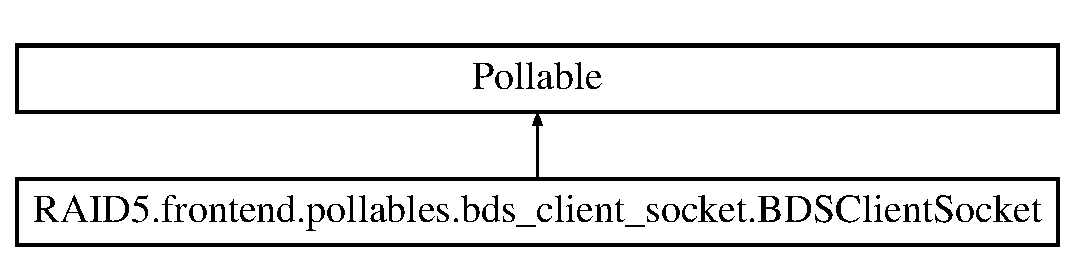
\includegraphics[height=2.000000cm]{class_r_a_i_d5_1_1frontend_1_1pollables_1_1bds__client__socket_1_1_b_d_s_client_socket}
\end{center}
\end{figure}
\subsection*{Public Member Functions}
\begin{DoxyCompactItemize}
\item 
\mbox{\Hypertarget{class_r_a_i_d5_1_1frontend_1_1pollables_1_1bds__client__socket_1_1_b_d_s_client_socket_a5bd07e24043c51439aea13f04d06737d}\label{class_r_a_i_d5_1_1frontend_1_1pollables_1_1bds__client__socket_1_1_b_d_s_client_socket_a5bd07e24043c51439aea13f04d06737d}} 
def {\bfseries \+\_\+\+\_\+init\+\_\+\+\_\+} (self, socket, client\+\_\+context, client\+\_\+update, parent)
\item 
\mbox{\Hypertarget{class_r_a_i_d5_1_1frontend_1_1pollables_1_1bds__client__socket_1_1_b_d_s_client_socket_a2fc48ec95e28cc6731de9d298b05acfd}\label{class_r_a_i_d5_1_1frontend_1_1pollables_1_1bds__client__socket_1_1_b_d_s_client_socket_a2fc48ec95e28cc6731de9d298b05acfd}} 
def {\bfseries is\+\_\+terminating} (self)
\item 
\mbox{\Hypertarget{class_r_a_i_d5_1_1frontend_1_1pollables_1_1bds__client__socket_1_1_b_d_s_client_socket_a777b2fe7d558be9591b5d901364289dc}\label{class_r_a_i_d5_1_1frontend_1_1pollables_1_1bds__client__socket_1_1_b_d_s_client_socket_a777b2fe7d558be9591b5d901364289dc}} 
def {\bfseries state} (self)
\item 
\mbox{\Hypertarget{class_r_a_i_d5_1_1frontend_1_1pollables_1_1bds__client__socket_1_1_b_d_s_client_socket_a8d069b2bb110d9096bcfdc823963a1c7}\label{class_r_a_i_d5_1_1frontend_1_1pollables_1_1bds__client__socket_1_1_b_d_s_client_socket_a8d069b2bb110d9096bcfdc823963a1c7}} 
def {\bfseries state} (self, s)
\item 
\mbox{\Hypertarget{class_r_a_i_d5_1_1frontend_1_1pollables_1_1bds__client__socket_1_1_b_d_s_client_socket_a560e18a6f2e66c1c4966909dbf2ad762}\label{class_r_a_i_d5_1_1frontend_1_1pollables_1_1bds__client__socket_1_1_b_d_s_client_socket_a560e18a6f2e66c1c4966909dbf2ad762}} 
def {\bfseries service} (self)
\item 
\mbox{\Hypertarget{class_r_a_i_d5_1_1frontend_1_1pollables_1_1bds__client__socket_1_1_b_d_s_client_socket_ae7942508c6c8d2310c1be2b128dee4c2}\label{class_r_a_i_d5_1_1frontend_1_1pollables_1_1bds__client__socket_1_1_b_d_s_client_socket_ae7942508c6c8d2310c1be2b128dee4c2}} 
def {\bfseries service} (self, s)
\item 
\mbox{\Hypertarget{class_r_a_i_d5_1_1frontend_1_1pollables_1_1bds__client__socket_1_1_b_d_s_client_socket_a2a7d10942f53e6c4c0a1891c98741e2e}\label{class_r_a_i_d5_1_1frontend_1_1pollables_1_1bds__client__socket_1_1_b_d_s_client_socket_a2a7d10942f53e6c4c0a1891c98741e2e}} 
def {\bfseries parent} (self)
\item 
\mbox{\Hypertarget{class_r_a_i_d5_1_1frontend_1_1pollables_1_1bds__client__socket_1_1_b_d_s_client_socket_a47a08215123f34ac74ec97b5ac6492cd}\label{class_r_a_i_d5_1_1frontend_1_1pollables_1_1bds__client__socket_1_1_b_d_s_client_socket_a47a08215123f34ac74ec97b5ac6492cd}} 
def {\bfseries parent} (self, p)
\item 
\mbox{\Hypertarget{class_r_a_i_d5_1_1frontend_1_1pollables_1_1bds__client__socket_1_1_b_d_s_client_socket_a5c5dcd760c380c0d22e3ad59fdd3c7e3}\label{class_r_a_i_d5_1_1frontend_1_1pollables_1_1bds__client__socket_1_1_b_d_s_client_socket_a5c5dcd760c380c0d22e3ad59fdd3c7e3}} 
def {\bfseries request\+\_\+context} (self)
\item 
\mbox{\Hypertarget{class_r_a_i_d5_1_1frontend_1_1pollables_1_1bds__client__socket_1_1_b_d_s_client_socket_acd5944034b25ec7ccca0626f16c27c24}\label{class_r_a_i_d5_1_1frontend_1_1pollables_1_1bds__client__socket_1_1_b_d_s_client_socket_acd5944034b25ec7ccca0626f16c27c24}} 
def {\bfseries request\+\_\+context} (self, r)
\item 
\mbox{\Hypertarget{class_r_a_i_d5_1_1frontend_1_1pollables_1_1bds__client__socket_1_1_b_d_s_client_socket_a29c1025858836d19f7375a3d63f49602}\label{class_r_a_i_d5_1_1frontend_1_1pollables_1_1bds__client__socket_1_1_b_d_s_client_socket_a29c1025858836d19f7375a3d63f49602}} 
def {\bfseries application\+\_\+context} (self)
\item 
\mbox{\Hypertarget{class_r_a_i_d5_1_1frontend_1_1pollables_1_1bds__client__socket_1_1_b_d_s_client_socket_a7fb0f3093eb0241767f10dc17a98df3b}\label{class_r_a_i_d5_1_1frontend_1_1pollables_1_1bds__client__socket_1_1_b_d_s_client_socket_a7fb0f3093eb0241767f10dc17a98df3b}} 
def {\bfseries application\+\_\+context} (self, a)
\item 
\mbox{\Hypertarget{class_r_a_i_d5_1_1frontend_1_1pollables_1_1bds__client__socket_1_1_b_d_s_client_socket_a0605ecc40175b37dde7247db4e022f3f}\label{class_r_a_i_d5_1_1frontend_1_1pollables_1_1bds__client__socket_1_1_b_d_s_client_socket_a0605ecc40175b37dde7247db4e022f3f}} 
def {\bfseries client\+\_\+update} (self)
\item 
\mbox{\Hypertarget{class_r_a_i_d5_1_1frontend_1_1pollables_1_1bds__client__socket_1_1_b_d_s_client_socket_a0b9807c825e2f55905dea25329da894a}\label{class_r_a_i_d5_1_1frontend_1_1pollables_1_1bds__client__socket_1_1_b_d_s_client_socket_a0b9807c825e2f55905dea25329da894a}} 
def {\bfseries client\+\_\+update} (self, c\+\_\+u)
\item 
\mbox{\Hypertarget{class_r_a_i_d5_1_1frontend_1_1pollables_1_1bds__client__socket_1_1_b_d_s_client_socket_a84c12e1e133fc3c9247a5a33f775b295}\label{class_r_a_i_d5_1_1frontend_1_1pollables_1_1bds__client__socket_1_1_b_d_s_client_socket_a84c12e1e133fc3c9247a5a33f775b295}} 
def {\bfseries recvd\+\_\+data} (self)
\item 
\mbox{\Hypertarget{class_r_a_i_d5_1_1frontend_1_1pollables_1_1bds__client__socket_1_1_b_d_s_client_socket_ad998f9d6ba32f35766a590ee8f36e3df}\label{class_r_a_i_d5_1_1frontend_1_1pollables_1_1bds__client__socket_1_1_b_d_s_client_socket_ad998f9d6ba32f35766a590ee8f36e3df}} 
def {\bfseries recvd\+\_\+data} (self, r)
\item 
\mbox{\Hypertarget{class_r_a_i_d5_1_1frontend_1_1pollables_1_1bds__client__socket_1_1_b_d_s_client_socket_a11ad8ce20fa8f0ae7ca19e8a52e97a46}\label{class_r_a_i_d5_1_1frontend_1_1pollables_1_1bds__client__socket_1_1_b_d_s_client_socket_a11ad8ce20fa8f0ae7ca19e8a52e97a46}} 
def {\bfseries data\+\_\+to\+\_\+send} (self)
\item 
\mbox{\Hypertarget{class_r_a_i_d5_1_1frontend_1_1pollables_1_1bds__client__socket_1_1_b_d_s_client_socket_a34e6838b87a0e20a5e75e09a65f5ae1a}\label{class_r_a_i_d5_1_1frontend_1_1pollables_1_1bds__client__socket_1_1_b_d_s_client_socket_a34e6838b87a0e20a5e75e09a65f5ae1a}} 
def {\bfseries data\+\_\+to\+\_\+send} (self, d)
\item 
\mbox{\Hypertarget{class_r_a_i_d5_1_1frontend_1_1pollables_1_1bds__client__socket_1_1_b_d_s_client_socket_af09734344f36f6fcfbed05a25f19ee79}\label{class_r_a_i_d5_1_1frontend_1_1pollables_1_1bds__client__socket_1_1_b_d_s_client_socket_af09734344f36f6fcfbed05a25f19ee79}} 
def {\bfseries socket} (self)
\item 
\mbox{\Hypertarget{class_r_a_i_d5_1_1frontend_1_1pollables_1_1bds__client__socket_1_1_b_d_s_client_socket_ad5f50b0f3923f5bebfef570851af7682}\label{class_r_a_i_d5_1_1frontend_1_1pollables_1_1bds__client__socket_1_1_b_d_s_client_socket_ad5f50b0f3923f5bebfef570851af7682}} 
def {\bfseries fd} (self)
\item 
\mbox{\Hypertarget{class_r_a_i_d5_1_1frontend_1_1pollables_1_1bds__client__socket_1_1_b_d_s_client_socket_a62c2bb5e93d9a6ebd64d039fc10b432c}\label{class_r_a_i_d5_1_1frontend_1_1pollables_1_1bds__client__socket_1_1_b_d_s_client_socket_a62c2bb5e93d9a6ebd64d039fc10b432c}} 
def {\bfseries on\+\_\+close} (self)
\item 
\mbox{\Hypertarget{class_r_a_i_d5_1_1frontend_1_1pollables_1_1bds__client__socket_1_1_b_d_s_client_socket_a0f90e9e9fd67d03701a2f7fc524fd4fb}\label{class_r_a_i_d5_1_1frontend_1_1pollables_1_1bds__client__socket_1_1_b_d_s_client_socket_a0f90e9e9fd67d03701a2f7fc524fd4fb}} 
def {\bfseries on\+\_\+read} (self)
\item 
\mbox{\Hypertarget{class_r_a_i_d5_1_1frontend_1_1pollables_1_1bds__client__socket_1_1_b_d_s_client_socket_a6c80bd3174775d419d7c192df6e5592e}\label{class_r_a_i_d5_1_1frontend_1_1pollables_1_1bds__client__socket_1_1_b_d_s_client_socket_a6c80bd3174775d419d7c192df6e5592e}} 
def {\bfseries on\+\_\+error} (self)
\item 
\mbox{\Hypertarget{class_r_a_i_d5_1_1frontend_1_1pollables_1_1bds__client__socket_1_1_b_d_s_client_socket_a1a16548e7af22709b00d1be9a2d54cdd}\label{class_r_a_i_d5_1_1frontend_1_1pollables_1_1bds__client__socket_1_1_b_d_s_client_socket_a1a16548e7af22709b00d1be9a2d54cdd}} 
def {\bfseries on\+\_\+write} (self)
\item 
\mbox{\Hypertarget{class_r_a_i_d5_1_1frontend_1_1pollables_1_1bds__client__socket_1_1_b_d_s_client_socket_a3350cf0aac6f5142cfbc6f540ee72d4f}\label{class_r_a_i_d5_1_1frontend_1_1pollables_1_1bds__client__socket_1_1_b_d_s_client_socket_a3350cf0aac6f5142cfbc6f540ee72d4f}} 
def {\bfseries get\+\_\+events} (self)
\item 
\mbox{\Hypertarget{class_r_a_i_d5_1_1frontend_1_1pollables_1_1bds__client__socket_1_1_b_d_s_client_socket_a5b0237d7d6164f65ddfcf49c9f6e325e}\label{class_r_a_i_d5_1_1frontend_1_1pollables_1_1bds__client__socket_1_1_b_d_s_client_socket_a5b0237d7d6164f65ddfcf49c9f6e325e}} 
def {\bfseries \+\_\+\+\_\+repr\+\_\+\+\_\+} (self)
\end{DoxyCompactItemize}
\subsection*{Static Public Attributes}
\begin{DoxyCompactItemize}
\item 
dictionary {\bfseries states}
\end{DoxyCompactItemize}


\subsection{Member Data Documentation}
\mbox{\Hypertarget{class_r_a_i_d5_1_1frontend_1_1pollables_1_1bds__client__socket_1_1_b_d_s_client_socket_a50f89a58166b0f6f7c1f8097f3bdb73a}\label{class_r_a_i_d5_1_1frontend_1_1pollables_1_1bds__client__socket_1_1_b_d_s_client_socket_a50f89a58166b0f6f7c1f8097f3bdb73a}} 
\index{R\+A\+I\+D5\+::frontend\+::pollables\+::bds\+\_\+client\+\_\+socket\+::\+B\+D\+S\+Client\+Socket@{R\+A\+I\+D5\+::frontend\+::pollables\+::bds\+\_\+client\+\_\+socket\+::\+B\+D\+S\+Client\+Socket}!states@{states}}
\index{states@{states}!R\+A\+I\+D5\+::frontend\+::pollables\+::bds\+\_\+client\+\_\+socket\+::\+B\+D\+S\+Client\+Socket@{R\+A\+I\+D5\+::frontend\+::pollables\+::bds\+\_\+client\+\_\+socket\+::\+B\+D\+S\+Client\+Socket}}
\subsubsection{\texorpdfstring{states}{states}}
{\footnotesize\ttfamily dictionary R\+A\+I\+D5.\+frontend.\+pollables.\+bds\+\_\+client\+\_\+socket.\+B\+D\+S\+Client\+Socket.\+states\hspace{0.3cm}{\ttfamily [static]}}

{\bfseries Initial value\+:}
\begin{DoxyCode}
=  \{
        constants.SEND\_REQUEST\_STATE: \{
            \textcolor{stringliteral}{"function"}: http\_util.send\_request\_state,
            \textcolor{stringliteral}{"next"}: constants.SEND\_HEADERS\_STATE,
        \},
        constants.SEND\_HEADERS\_STATE: \{
            \textcolor{stringliteral}{"function"}: http\_util.send\_headers\_state,
            \textcolor{stringliteral}{"next"}: constants.SEND\_CONTENT\_STATE,
        \},
        constants.SEND\_CONTENT\_STATE: \{
            \textcolor{stringliteral}{"function"}: http\_util.send\_content\_state,
            \textcolor{stringliteral}{"next"}: constants.GET\_STATUS\_STATE,
        \},
        constants.GET\_STATUS\_STATE: \{
            \textcolor{stringliteral}{"function"}: http\_util.get\_status\_state,
            \textcolor{stringliteral}{"next"}: constants.GET\_HEADERS\_STATE
        \},
        constants.GET\_HEADERS\_STATE: \{
            \textcolor{stringliteral}{"function"}: http\_util.get\_headers\_state,
            \textcolor{stringliteral}{"next"}: constants.GET\_CONTENT\_STATE
        \},
        constants.GET\_CONTENT\_STATE: \{
            \textcolor{stringliteral}{"function"}: http\_util.get\_content\_state,
            \textcolor{stringliteral}{"next"}: constants.CLOSING\_STATE
        \},
        constants.CLOSING\_STATE: \{
            \textcolor{stringliteral}{"next"}: constants.CLOSING\_STATE,
        \}
    \}
\end{DoxyCode}


The documentation for this class was generated from the following file\+:\begin{DoxyCompactItemize}
\item 
C\+:/cygwin64/tmp/\+R\+A\+I\+D5/frontend/pollables/bds\+\_\+client\+\_\+socket.\+py\end{DoxyCompactItemize}

\hypertarget{class_r_a_i_d5_1_1frontend_1_1utilities_1_1cache_1_1_cache}{}\section{R\+A\+I\+D5.\+frontend.\+utilities.\+cache.\+Cache Class Reference}
\label{class_r_a_i_d5_1_1frontend_1_1utilities_1_1cache_1_1_cache}\index{R\+A\+I\+D5.\+frontend.\+utilities.\+cache.\+Cache@{R\+A\+I\+D5.\+frontend.\+utilities.\+cache.\+Cache}}
Inheritance diagram for R\+A\+I\+D5.\+frontend.\+utilities.\+cache.\+Cache\+:\begin{figure}[H]
\begin{center}
\leavevmode
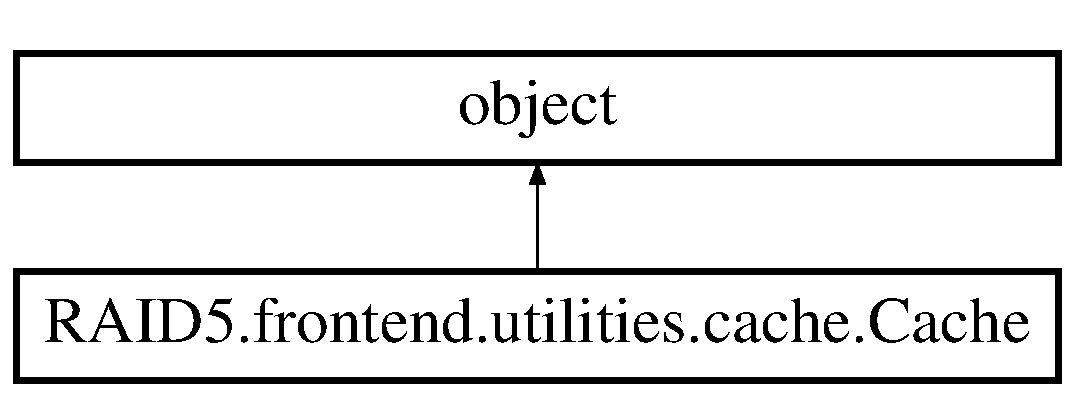
\includegraphics[height=2.000000cm]{class_r_a_i_d5_1_1frontend_1_1utilities_1_1cache_1_1_cache}
\end{center}
\end{figure}
\subsection*{Public Member Functions}
\begin{DoxyCompactItemize}
\item 
\mbox{\Hypertarget{class_r_a_i_d5_1_1frontend_1_1utilities_1_1cache_1_1_cache_aa1a1e8c4bf1e2e10224bdd124d2874c1}\label{class_r_a_i_d5_1_1frontend_1_1utilities_1_1cache_1_1_cache_aa1a1e8c4bf1e2e10224bdd124d2874c1}} 
def {\bfseries \+\_\+\+\_\+init\+\_\+\+\_\+} (self, mode=D\+O\+R\+M\+A\+N\+T\+\_\+\+M\+O\+DE)
\item 
\mbox{\Hypertarget{class_r_a_i_d5_1_1frontend_1_1utilities_1_1cache_1_1_cache_ac2ec2ccc654768bc9afdc8a6552681cf}\label{class_r_a_i_d5_1_1frontend_1_1utilities_1_1cache_1_1_cache_ac2ec2ccc654768bc9afdc8a6552681cf}} 
def {\bfseries mode} (self)
\item 
\mbox{\Hypertarget{class_r_a_i_d5_1_1frontend_1_1utilities_1_1cache_1_1_cache_a278ce895da3167ad8576102fff9fede5}\label{class_r_a_i_d5_1_1frontend_1_1utilities_1_1cache_1_1_cache_a278ce895da3167ad8576102fff9fede5}} 
def {\bfseries mode} (self, m)
\item 
\mbox{\Hypertarget{class_r_a_i_d5_1_1frontend_1_1utilities_1_1cache_1_1_cache_ab8f1c597c18154b7b5719aa0da56886f}\label{class_r_a_i_d5_1_1frontend_1_1utilities_1_1cache_1_1_cache_ab8f1c597c18154b7b5719aa0da56886f}} 
def {\bfseries pointer} (self)
\item 
\mbox{\Hypertarget{class_r_a_i_d5_1_1frontend_1_1utilities_1_1cache_1_1_cache_ab8ad402b867bf7ea8ce26cd025b421a8}\label{class_r_a_i_d5_1_1frontend_1_1utilities_1_1cache_1_1_cache_ab8ad402b867bf7ea8ce26cd025b421a8}} 
def {\bfseries pointer} (self, p)
\item 
\mbox{\Hypertarget{class_r_a_i_d5_1_1frontend_1_1utilities_1_1cache_1_1_cache_a3975618f38fb33b1a993a6dd5ccfb450}\label{class_r_a_i_d5_1_1frontend_1_1utilities_1_1cache_1_1_cache_a3975618f38fb33b1a993a6dd5ccfb450}} 
def {\bfseries is\+\_\+empty} (self)
\item 
\mbox{\Hypertarget{class_r_a_i_d5_1_1frontend_1_1utilities_1_1cache_1_1_cache_ad5d7181d9baa78638d489d75ac20ad43}\label{class_r_a_i_d5_1_1frontend_1_1utilities_1_1cache_1_1_cache_ad5d7181d9baa78638d489d75ac20ad43}} 
def {\bfseries size} (self)
\item 
\mbox{\Hypertarget{class_r_a_i_d5_1_1frontend_1_1utilities_1_1cache_1_1_cache_a244bfa5e40c85f2e7178e8a85f2bf5e8}\label{class_r_a_i_d5_1_1frontend_1_1utilities_1_1cache_1_1_cache_a244bfa5e40c85f2e7178e8a85f2bf5e8}} 
def {\bfseries get\+\_\+rebuild\+\_\+percentage} (self)
\item 
\mbox{\Hypertarget{class_r_a_i_d5_1_1frontend_1_1utilities_1_1cache_1_1_cache_a5ac35bef5b86de566c13e0cb0832dd67}\label{class_r_a_i_d5_1_1frontend_1_1utilities_1_1cache_1_1_cache_a5ac35bef5b86de566c13e0cb0832dd67}} 
def {\bfseries cache\+\_\+overflow} (self)
\item 
\mbox{\Hypertarget{class_r_a_i_d5_1_1frontend_1_1utilities_1_1cache_1_1_cache_a98196b88f82ad135c91e7efbdf168fcc}\label{class_r_a_i_d5_1_1frontend_1_1utilities_1_1cache_1_1_cache_a98196b88f82ad135c91e7efbdf168fcc}} 
def {\bfseries check\+\_\+if\+\_\+add} (self, block\+\_\+num)
\item 
\mbox{\Hypertarget{class_r_a_i_d5_1_1frontend_1_1utilities_1_1cache_1_1_cache_a261747ad7f810e40d7144f284e81ab82}\label{class_r_a_i_d5_1_1frontend_1_1utilities_1_1cache_1_1_cache_a261747ad7f810e40d7144f284e81ab82}} 
def {\bfseries add\+\_\+block} (self, block\+\_\+num, block\+\_\+data)
\item 
\mbox{\Hypertarget{class_r_a_i_d5_1_1frontend_1_1utilities_1_1cache_1_1_cache_a83490907d4b89b8eb55adcee2724fcd8}\label{class_r_a_i_d5_1_1frontend_1_1utilities_1_1cache_1_1_cache_a83490907d4b89b8eb55adcee2724fcd8}} 
def {\bfseries next\+\_\+block} (self)
\item 
\mbox{\Hypertarget{class_r_a_i_d5_1_1frontend_1_1utilities_1_1cache_1_1_cache_ad17acc2c8e019c094731924aae02449f}\label{class_r_a_i_d5_1_1frontend_1_1utilities_1_1cache_1_1_cache_ad17acc2c8e019c094731924aae02449f}} 
def {\bfseries \+\_\+\+\_\+repr\+\_\+\+\_\+} (self)
\item 
\mbox{\Hypertarget{class_r_a_i_d5_1_1frontend_1_1utilities_1_1cache_1_1_cache_a3268ce895eebcfaa06390635d8f089e6}\label{class_r_a_i_d5_1_1frontend_1_1utilities_1_1cache_1_1_cache_a3268ce895eebcfaa06390635d8f089e6}} 
def {\bfseries change\+\_\+topology} (self)
\end{DoxyCompactItemize}
\subsection*{Static Public Attributes}
\begin{DoxyCompactItemize}
\item 
dictionary {\bfseries M\+O\+D\+E\+\_\+\+N\+A\+M\+ES}
\end{DoxyCompactItemize}


\subsection{Member Data Documentation}
\mbox{\Hypertarget{class_r_a_i_d5_1_1frontend_1_1utilities_1_1cache_1_1_cache_aaa21f9f1cae2d6df8f9ffaab0f0230e0}\label{class_r_a_i_d5_1_1frontend_1_1utilities_1_1cache_1_1_cache_aaa21f9f1cae2d6df8f9ffaab0f0230e0}} 
\index{R\+A\+I\+D5\+::frontend\+::utilities\+::cache\+::\+Cache@{R\+A\+I\+D5\+::frontend\+::utilities\+::cache\+::\+Cache}!M\+O\+D\+E\+\_\+\+N\+A\+M\+ES@{M\+O\+D\+E\+\_\+\+N\+A\+M\+ES}}
\index{M\+O\+D\+E\+\_\+\+N\+A\+M\+ES@{M\+O\+D\+E\+\_\+\+N\+A\+M\+ES}!R\+A\+I\+D5\+::frontend\+::utilities\+::cache\+::\+Cache@{R\+A\+I\+D5\+::frontend\+::utilities\+::cache\+::\+Cache}}
\subsubsection{\texorpdfstring{M\+O\+D\+E\+\_\+\+N\+A\+M\+ES}{MODE\_NAMES}}
{\footnotesize\ttfamily dictionary R\+A\+I\+D5.\+frontend.\+utilities.\+cache.\+Cache.\+M\+O\+D\+E\+\_\+\+N\+A\+M\+ES\hspace{0.3cm}{\ttfamily [static]}}

{\bfseries Initial value\+:}
\begin{DoxyCode}
=  \{
        DORMANT\_MODE: \textcolor{stringliteral}{"DORMANT MODE"},
        CACHE\_MODE: \textcolor{stringliteral}{"CACHE MODE"},
        SCRATCH\_MODE: \textcolor{stringliteral}{"SCRATCH MODE"},
    \}
\end{DoxyCode}


The documentation for this class was generated from the following file\+:\begin{DoxyCompactItemize}
\item 
C\+:/cygwin64/tmp/\+R\+A\+I\+D5/frontend/utilities/cache.\+py\end{DoxyCompactItemize}

\hypertarget{class_r_a_i_d5_1_1common_1_1pollables_1_1callable_1_1_callable}{}\section{R\+A\+I\+D5.\+common.\+pollables.\+callable.\+Callable Class Reference}
\label{class_r_a_i_d5_1_1common_1_1pollables_1_1callable_1_1_callable}\index{R\+A\+I\+D5.\+common.\+pollables.\+callable.\+Callable@{R\+A\+I\+D5.\+common.\+pollables.\+callable.\+Callable}}
Inheritance diagram for R\+A\+I\+D5.\+common.\+pollables.\+callable.\+Callable\+:\begin{figure}[H]
\begin{center}
\leavevmode
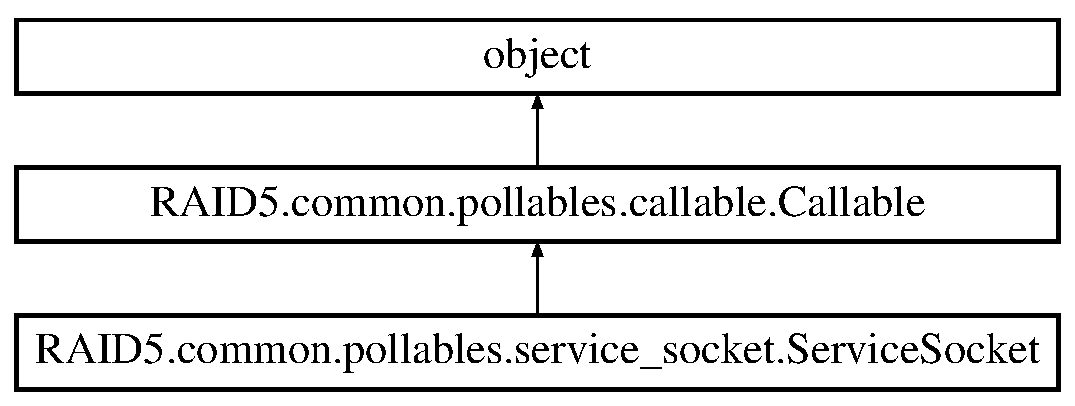
\includegraphics[height=3.000000cm]{class_r_a_i_d5_1_1common_1_1pollables_1_1callable_1_1_callable}
\end{center}
\end{figure}
\subsection*{Public Member Functions}
\begin{DoxyCompactItemize}
\item 
\mbox{\Hypertarget{class_r_a_i_d5_1_1common_1_1pollables_1_1callable_1_1_callable_a96d895077ba8cfbfa9afb798634de294}\label{class_r_a_i_d5_1_1common_1_1pollables_1_1callable_1_1_callable_a96d895077ba8cfbfa9afb798634de294}} 
def {\bfseries on\+\_\+finish} (self)
\end{DoxyCompactItemize}


The documentation for this class was generated from the following file\+:\begin{DoxyCompactItemize}
\item 
C\+:/cygwin64/tmp/\+R\+A\+I\+D5/common/pollables/callable.\+py\end{DoxyCompactItemize}

\hypertarget{class_r_a_i_d5_1_1frontend_1_1services_1_1client__services_1_1_client_service}{}\section{R\+A\+I\+D5.\+frontend.\+services.\+client\+\_\+services.\+Client\+Service Class Reference}
\label{class_r_a_i_d5_1_1frontend_1_1services_1_1client__services_1_1_client_service}\index{R\+A\+I\+D5.\+frontend.\+services.\+client\+\_\+services.\+Client\+Service@{R\+A\+I\+D5.\+frontend.\+services.\+client\+\_\+services.\+Client\+Service}}
Inheritance diagram for R\+A\+I\+D5.\+frontend.\+services.\+client\+\_\+services.\+Client\+Service\+:\begin{figure}[H]
\begin{center}
\leavevmode
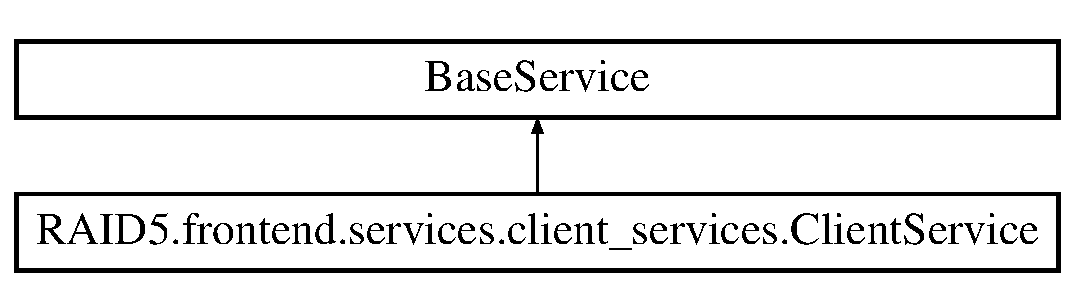
\includegraphics[height=2.000000cm]{class_r_a_i_d5_1_1frontend_1_1services_1_1client__services_1_1_client_service}
\end{center}
\end{figure}
\subsection*{Public Member Functions}
\begin{DoxyCompactItemize}
\item 
\mbox{\Hypertarget{class_r_a_i_d5_1_1frontend_1_1services_1_1client__services_1_1_client_service_a8f006fd47ed59eb687f4e23cd7cf1850}\label{class_r_a_i_d5_1_1frontend_1_1services_1_1client__services_1_1_client_service_a8f006fd47ed59eb687f4e23cd7cf1850}} 
def {\bfseries \+\_\+\+\_\+init\+\_\+\+\_\+} (self, entry)
\item 
\mbox{\Hypertarget{class_r_a_i_d5_1_1frontend_1_1services_1_1client__services_1_1_client_service_a86cd6e3f4af08083be74465aaf11e89a}\label{class_r_a_i_d5_1_1frontend_1_1services_1_1client__services_1_1_client_service_a86cd6e3f4af08083be74465aaf11e89a}} 
def {\bfseries handle\+\_\+content} (self, entry, content)
\item 
\mbox{\Hypertarget{class_r_a_i_d5_1_1frontend_1_1services_1_1client__services_1_1_client_service_a460750a7548083eb5907d78c54f41452}\label{class_r_a_i_d5_1_1frontend_1_1services_1_1client__services_1_1_client_service_a460750a7548083eb5907d78c54f41452}} 
def {\bfseries before\+\_\+terminate} (self, entry)
\end{DoxyCompactItemize}
\subsection*{Static Public Member Functions}
\begin{DoxyCompactItemize}
\item 
\mbox{\Hypertarget{class_r_a_i_d5_1_1frontend_1_1services_1_1client__services_1_1_client_service_a12e248f08e8568259ff490c8da577f7e}\label{class_r_a_i_d5_1_1frontend_1_1services_1_1client__services_1_1_client_service_a12e248f08e8568259ff490c8da577f7e}} 
def {\bfseries get\+\_\+name} ()
\end{DoxyCompactItemize}


The documentation for this class was generated from the following file\+:\begin{DoxyCompactItemize}
\item 
C\+:/cygwin64/tmp/\+R\+A\+I\+D5/frontend/services/client\+\_\+services.\+py\end{DoxyCompactItemize}

\hypertarget{class_r_a_i_d5_1_1frontend_1_1services_1_1connect__service_1_1_connect_service}{}\section{R\+A\+I\+D5.\+frontend.\+services.\+connect\+\_\+service.\+Connect\+Service Class Reference}
\label{class_r_a_i_d5_1_1frontend_1_1services_1_1connect__service_1_1_connect_service}\index{R\+A\+I\+D5.\+frontend.\+services.\+connect\+\_\+service.\+Connect\+Service@{R\+A\+I\+D5.\+frontend.\+services.\+connect\+\_\+service.\+Connect\+Service}}
Inheritance diagram for R\+A\+I\+D5.\+frontend.\+services.\+connect\+\_\+service.\+Connect\+Service\+:\begin{figure}[H]
\begin{center}
\leavevmode
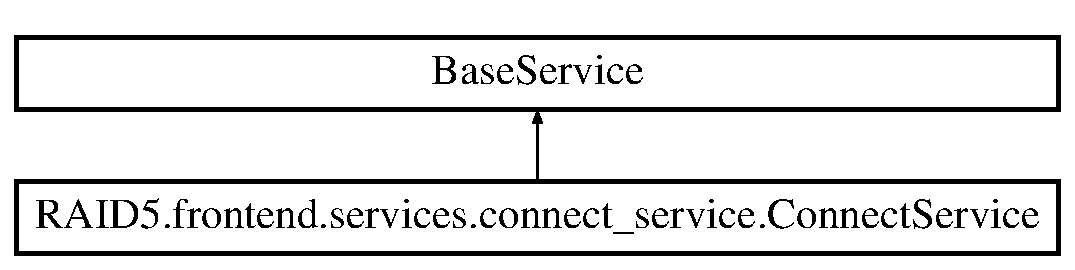
\includegraphics[height=2.000000cm]{class_r_a_i_d5_1_1frontend_1_1services_1_1connect__service_1_1_connect_service}
\end{center}
\end{figure}
\subsection*{Public Member Functions}
\begin{DoxyCompactItemize}
\item 
\mbox{\Hypertarget{class_r_a_i_d5_1_1frontend_1_1services_1_1connect__service_1_1_connect_service_a6218d1dca1455abab739ecc5d3520cdd}\label{class_r_a_i_d5_1_1frontend_1_1services_1_1connect__service_1_1_connect_service_a6218d1dca1455abab739ecc5d3520cdd}} 
def {\bfseries \+\_\+\+\_\+init\+\_\+\+\_\+} (self, entry, socket\+\_\+data, args)
\item 
\mbox{\Hypertarget{class_r_a_i_d5_1_1frontend_1_1services_1_1connect__service_1_1_connect_service_ae23c53fa0cc7b350fa07f1f844ff1287}\label{class_r_a_i_d5_1_1frontend_1_1services_1_1connect__service_1_1_connect_service_ae23c53fa0cc7b350fa07f1f844ff1287}} 
def {\bfseries initial\+\_\+setup} (self, entry)
\item 
\mbox{\Hypertarget{class_r_a_i_d5_1_1frontend_1_1services_1_1connect__service_1_1_connect_service_af0dcf4058503e52eaa1aefb988157689}\label{class_r_a_i_d5_1_1frontend_1_1services_1_1connect__service_1_1_connect_service_af0dcf4058503e52eaa1aefb988157689}} 
def {\bfseries before\+\_\+response\+\_\+status} (self, entry)
\item 
\mbox{\Hypertarget{class_r_a_i_d5_1_1frontend_1_1services_1_1connect__service_1_1_connect_service_acbf976ac298fcdfa691333de9ad5919a}\label{class_r_a_i_d5_1_1frontend_1_1services_1_1connect__service_1_1_connect_service_acbf976ac298fcdfa691333de9ad5919a}} 
def {\bfseries before\+\_\+get\+\_\+data} (self, entry)
\item 
\mbox{\Hypertarget{class_r_a_i_d5_1_1frontend_1_1services_1_1connect__service_1_1_connect_service_aed581c478f4b16756b7a7a0c571c6bb6}\label{class_r_a_i_d5_1_1frontend_1_1services_1_1connect__service_1_1_connect_service_aed581c478f4b16756b7a7a0c571c6bb6}} 
def {\bfseries after\+\_\+get\+\_\+data} (self, entry)
\item 
\mbox{\Hypertarget{class_r_a_i_d5_1_1frontend_1_1services_1_1connect__service_1_1_connect_service_a9c27f801f017751a69857ba96520f110}\label{class_r_a_i_d5_1_1frontend_1_1services_1_1connect__service_1_1_connect_service_a9c27f801f017751a69857ba96520f110}} 
def {\bfseries before\+\_\+set\+\_\+data} (self, entry)
\item 
\mbox{\Hypertarget{class_r_a_i_d5_1_1frontend_1_1services_1_1connect__service_1_1_connect_service_acddfbe6d4650b81fc365e42ca057f62f}\label{class_r_a_i_d5_1_1frontend_1_1services_1_1connect__service_1_1_connect_service_acddfbe6d4650b81fc365e42ca057f62f}} 
def {\bfseries after\+\_\+set\+\_\+data} (self, entry)
\item 
\mbox{\Hypertarget{class_r_a_i_d5_1_1frontend_1_1services_1_1connect__service_1_1_connect_service_a3fb1b717ca5f27b15841b817caf62d5e}\label{class_r_a_i_d5_1_1frontend_1_1services_1_1connect__service_1_1_connect_service_a3fb1b717ca5f27b15841b817caf62d5e}} 
def {\bfseries before\+\_\+update\+\_\+level} (self, entry)
\item 
\mbox{\Hypertarget{class_r_a_i_d5_1_1frontend_1_1services_1_1connect__service_1_1_connect_service_ab9c25f4a46f8864b5f0190c62a710866}\label{class_r_a_i_d5_1_1frontend_1_1services_1_1connect__service_1_1_connect_service_ab9c25f4a46f8864b5f0190c62a710866}} 
def {\bfseries after\+\_\+update\+\_\+level} (self, entry)
\item 
\mbox{\Hypertarget{class_r_a_i_d5_1_1frontend_1_1services_1_1connect__service_1_1_connect_service_a25174f4a8af218662a71cd7544c2ee74}\label{class_r_a_i_d5_1_1frontend_1_1services_1_1connect__service_1_1_connect_service_a25174f4a8af218662a71cd7544c2ee74}} 
def {\bfseries before\+\_\+terminate} (self, entry)
\item 
\mbox{\Hypertarget{class_r_a_i_d5_1_1frontend_1_1services_1_1connect__service_1_1_connect_service_a47aacb72236592742faad9fd77040130}\label{class_r_a_i_d5_1_1frontend_1_1services_1_1connect__service_1_1_connect_service_a47aacb72236592742faad9fd77040130}} 
def {\bfseries on\+\_\+finish} (self, entry)
\item 
\mbox{\Hypertarget{class_r_a_i_d5_1_1frontend_1_1services_1_1connect__service_1_1_connect_service_a433716ef9ee81d170cf712912d1e67ba}\label{class_r_a_i_d5_1_1frontend_1_1services_1_1connect__service_1_1_connect_service_a433716ef9ee81d170cf712912d1e67ba}} 
def {\bfseries check\+\_\+if\+\_\+built} (self)
\end{DoxyCompactItemize}
\subsection*{Static Public Member Functions}
\begin{DoxyCompactItemize}
\item 
\mbox{\Hypertarget{class_r_a_i_d5_1_1frontend_1_1services_1_1connect__service_1_1_connect_service_aca07a530b6f670da26c3d0d2f402116b}\label{class_r_a_i_d5_1_1frontend_1_1services_1_1connect__service_1_1_connect_service_aca07a530b6f670da26c3d0d2f402116b}} 
def {\bfseries get\+\_\+name} ()
\end{DoxyCompactItemize}
\subsection*{Static Public Attributes}
\begin{DoxyCompactItemize}
\item 
list {\bfseries S\+T\+A\+T\+ES}
\end{DoxyCompactItemize}


\subsection{Member Data Documentation}
\mbox{\Hypertarget{class_r_a_i_d5_1_1frontend_1_1services_1_1connect__service_1_1_connect_service_a142f71d2cf709124f605a8e72729be2a}\label{class_r_a_i_d5_1_1frontend_1_1services_1_1connect__service_1_1_connect_service_a142f71d2cf709124f605a8e72729be2a}} 
\index{R\+A\+I\+D5\+::frontend\+::services\+::connect\+\_\+service\+::\+Connect\+Service@{R\+A\+I\+D5\+::frontend\+::services\+::connect\+\_\+service\+::\+Connect\+Service}!S\+T\+A\+T\+ES@{S\+T\+A\+T\+ES}}
\index{S\+T\+A\+T\+ES@{S\+T\+A\+T\+ES}!R\+A\+I\+D5\+::frontend\+::services\+::connect\+\_\+service\+::\+Connect\+Service@{R\+A\+I\+D5\+::frontend\+::services\+::connect\+\_\+service\+::\+Connect\+Service}}
\subsubsection{\texorpdfstring{S\+T\+A\+T\+ES}{STATES}}
{\footnotesize\ttfamily list R\+A\+I\+D5.\+frontend.\+services.\+connect\+\_\+service.\+Connect\+Service.\+S\+T\+A\+T\+ES\hspace{0.3cm}{\ttfamily [static]}}

{\bfseries Initial value\+:}
\begin{DoxyCode}
=  [
        \hyperlink{classstate_1_1_state}{state.State}(
            GET\_DATA\_STATE,
            [SET\_DATA\_STATE],
            before\_get\_data,
            after\_get\_data,
        ),
        \hyperlink{classstate_1_1_state}{state.State}(
            SET\_DATA\_STATE,
            [GET\_DATA\_STATE, UPDATE\_LEVEL\_STATE],
            before\_set\_data,
            after\_set\_data,
        ),
        \hyperlink{classstate_1_1_state}{state.State}(
            UPDATE\_LEVEL\_STATE,
            [FINAL\_STATE],
            before\_update\_level,
            after\_update\_level,
        ),
        \hyperlink{classstate_1_1_state}{state.State}(
            FINAL\_STATE,
            [FINAL\_STATE],
        ),
    ]
\end{DoxyCode}


The documentation for this class was generated from the following file\+:\begin{DoxyCompactItemize}
\item 
C\+:/cygwin64/tmp/\+R\+A\+I\+D5/frontend/services/connect\+\_\+service.\+py\end{DoxyCompactItemize}

\hypertarget{class_r_a_i_d5_1_1block__device_1_1pollables_1_1declarer__socket_1_1_declarer_socket}{}\section{R\+A\+I\+D5.\+block\+\_\+device.\+pollables.\+declarer\+\_\+socket.\+Declarer\+Socket Class Reference}
\label{class_r_a_i_d5_1_1block__device_1_1pollables_1_1declarer__socket_1_1_declarer_socket}\index{R\+A\+I\+D5.\+block\+\_\+device.\+pollables.\+declarer\+\_\+socket.\+Declarer\+Socket@{R\+A\+I\+D5.\+block\+\_\+device.\+pollables.\+declarer\+\_\+socket.\+Declarer\+Socket}}


A Block Device Socket that declares the server using U\+DP Multicast to other Frontend Servers to recognize.  


Inheritance diagram for R\+A\+I\+D5.\+block\+\_\+device.\+pollables.\+declarer\+\_\+socket.\+Declarer\+Socket\+:\begin{figure}[H]
\begin{center}
\leavevmode
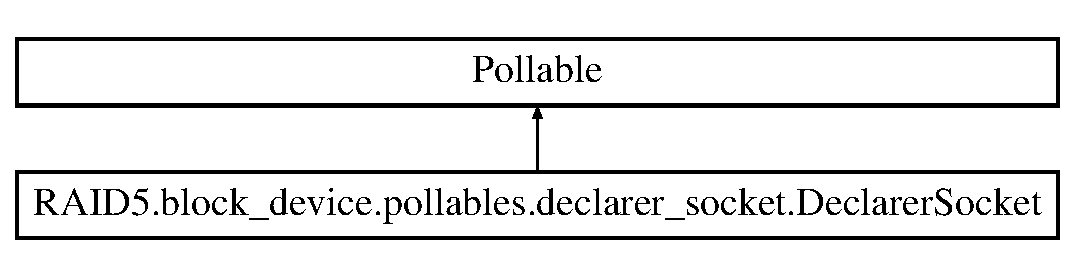
\includegraphics[height=2.000000cm]{class_r_a_i_d5_1_1block__device_1_1pollables_1_1declarer__socket_1_1_declarer_socket}
\end{center}
\end{figure}
\subsection*{Public Member Functions}
\begin{DoxyCompactItemize}
\item 
def \hyperlink{class_r_a_i_d5_1_1block__device_1_1pollables_1_1declarer__socket_1_1_declarer_socket_a0da7f9ba5573de93db76bd439e2aea6a}{\+\_\+\+\_\+init\+\_\+\+\_\+} (self, \hyperlink{class_r_a_i_d5_1_1block__device_1_1pollables_1_1declarer__socket_1_1_declarer_socket_ae5cf6477968fe119eed756e117ed2db2}{socket}, application\+\_\+context)
\begin{DoxyCompactList}\small\item\em Constructor for Declare\+Socket. \end{DoxyCompactList}\item 
\mbox{\Hypertarget{class_r_a_i_d5_1_1block__device_1_1pollables_1_1declarer__socket_1_1_declarer_socket_a379743c1568dc3f74d2b449ddabfbf58}\label{class_r_a_i_d5_1_1block__device_1_1pollables_1_1declarer__socket_1_1_declarer_socket_a379743c1568dc3f74d2b449ddabfbf58}} 
def \hyperlink{class_r_a_i_d5_1_1block__device_1_1pollables_1_1declarer__socket_1_1_declarer_socket_a379743c1568dc3f74d2b449ddabfbf58}{on\+\_\+idle} (self)
\begin{DoxyCompactList}\small\item\em Function that specifies what socket is to do when system is on\+\_\+idle declares itself using multicast. \end{DoxyCompactList}\item 
\mbox{\Hypertarget{class_r_a_i_d5_1_1block__device_1_1pollables_1_1declarer__socket_1_1_declarer_socket_a24329fed18e547225275086cfa45d98a}\label{class_r_a_i_d5_1_1block__device_1_1pollables_1_1declarer__socket_1_1_declarer_socket_a24329fed18e547225275086cfa45d98a}} 
def \hyperlink{class_r_a_i_d5_1_1block__device_1_1pollables_1_1declarer__socket_1_1_declarer_socket_a24329fed18e547225275086cfa45d98a}{create\+\_\+content} (self)
\begin{DoxyCompactList}\small\item\em Creates the decleration content. \end{DoxyCompactList}\item 
\mbox{\Hypertarget{class_r_a_i_d5_1_1block__device_1_1pollables_1_1declarer__socket_1_1_declarer_socket_af352950a82cb5b16a342af8025a29c8a}\label{class_r_a_i_d5_1_1block__device_1_1pollables_1_1declarer__socket_1_1_declarer_socket_af352950a82cb5b16a342af8025a29c8a}} 
def \hyperlink{class_r_a_i_d5_1_1block__device_1_1pollables_1_1declarer__socket_1_1_declarer_socket_af352950a82cb5b16a342af8025a29c8a}{get\+\_\+events} (self)
\begin{DoxyCompactList}\small\item\em Specifies what events the socket listens to required by \hyperlink{class_r_a_i_d5_1_1common_1_1pollables_1_1pollable_1_1_pollable}{common.\+pollables.\+pollable.\+Pollable}. \end{DoxyCompactList}\item 
\mbox{\Hypertarget{class_r_a_i_d5_1_1block__device_1_1pollables_1_1declarer__socket_1_1_declarer_socket_a1dd67d80155aa3136dfcc719c9b3977d}\label{class_r_a_i_d5_1_1block__device_1_1pollables_1_1declarer__socket_1_1_declarer_socket_a1dd67d80155aa3136dfcc719c9b3977d}} 
def \hyperlink{class_r_a_i_d5_1_1block__device_1_1pollables_1_1declarer__socket_1_1_declarer_socket_a1dd67d80155aa3136dfcc719c9b3977d}{is\+\_\+terminating} (self)
\begin{DoxyCompactList}\small\item\em When \hyperlink{class_r_a_i_d5_1_1block__device_1_1pollables_1_1declarer__socket_1_1_declarer_socket}{Declarer\+Socket} is terminating required by \hyperlink{class_r_a_i_d5_1_1common_1_1pollables_1_1pollable_1_1_pollable}{common.\+pollables.\+pollable.\+Pollable} will not terminate as long as server is running. \end{DoxyCompactList}\item 
\mbox{\Hypertarget{class_r_a_i_d5_1_1block__device_1_1pollables_1_1declarer__socket_1_1_declarer_socket_ade8b017d1d5495b3389205af00303067}\label{class_r_a_i_d5_1_1block__device_1_1pollables_1_1declarer__socket_1_1_declarer_socket_ade8b017d1d5495b3389205af00303067}} 
def \hyperlink{class_r_a_i_d5_1_1block__device_1_1pollables_1_1declarer__socket_1_1_declarer_socket_ade8b017d1d5495b3389205af00303067}{on\+\_\+close} (self)
\begin{DoxyCompactList}\small\item\em What \hyperlink{class_r_a_i_d5_1_1block__device_1_1pollables_1_1declarer__socket_1_1_declarer_socket}{Declarer\+Socket} does on close required from common.\+pollables.\+pollable will not close as long as server is running. \end{DoxyCompactList}\item 
\mbox{\Hypertarget{class_r_a_i_d5_1_1block__device_1_1pollables_1_1declarer__socket_1_1_declarer_socket_ae5cf6477968fe119eed756e117ed2db2}\label{class_r_a_i_d5_1_1block__device_1_1pollables_1_1declarer__socket_1_1_declarer_socket_ae5cf6477968fe119eed756e117ed2db2}} 
def \hyperlink{class_r_a_i_d5_1_1block__device_1_1pollables_1_1declarer__socket_1_1_declarer_socket_ae5cf6477968fe119eed756e117ed2db2}{socket} (self)
\begin{DoxyCompactList}\small\item\em Socket property. \end{DoxyCompactList}\item 
\mbox{\Hypertarget{class_r_a_i_d5_1_1block__device_1_1pollables_1_1declarer__socket_1_1_declarer_socket_a389a320c5f7132d02c6be9b268bc247f}\label{class_r_a_i_d5_1_1block__device_1_1pollables_1_1declarer__socket_1_1_declarer_socket_a389a320c5f7132d02c6be9b268bc247f}} 
def \hyperlink{class_r_a_i_d5_1_1block__device_1_1pollables_1_1declarer__socket_1_1_declarer_socket_a389a320c5f7132d02c6be9b268bc247f}{fd} (self)
\begin{DoxyCompactList}\small\item\em File descriptor property. \end{DoxyCompactList}\item 
def \hyperlink{class_r_a_i_d5_1_1block__device_1_1pollables_1_1declarer__socket_1_1_declarer_socket_a86b05b1856efb3051b78b6562934ac24}{\+\_\+\+\_\+repr\+\_\+\+\_\+} (self)
\begin{DoxyCompactList}\small\item\em representatin of \hyperlink{class_r_a_i_d5_1_1block__device_1_1pollables_1_1declarer__socket_1_1_declarer_socket}{Declarer\+Socket} Object \end{DoxyCompactList}\end{DoxyCompactItemize}


\subsection{Detailed Description}
A Block Device Socket that declares the server using U\+DP Multicast to other Frontend Servers to recognize. 

\subsection{Constructor \& Destructor Documentation}
\mbox{\Hypertarget{class_r_a_i_d5_1_1block__device_1_1pollables_1_1declarer__socket_1_1_declarer_socket_a0da7f9ba5573de93db76bd439e2aea6a}\label{class_r_a_i_d5_1_1block__device_1_1pollables_1_1declarer__socket_1_1_declarer_socket_a0da7f9ba5573de93db76bd439e2aea6a}} 
\index{R\+A\+I\+D5\+::block\+\_\+device\+::pollables\+::declarer\+\_\+socket\+::\+Declarer\+Socket@{R\+A\+I\+D5\+::block\+\_\+device\+::pollables\+::declarer\+\_\+socket\+::\+Declarer\+Socket}!\+\_\+\+\_\+init\+\_\+\+\_\+@{\+\_\+\+\_\+init\+\_\+\+\_\+}}
\index{\+\_\+\+\_\+init\+\_\+\+\_\+@{\+\_\+\+\_\+init\+\_\+\+\_\+}!R\+A\+I\+D5\+::block\+\_\+device\+::pollables\+::declarer\+\_\+socket\+::\+Declarer\+Socket@{R\+A\+I\+D5\+::block\+\_\+device\+::pollables\+::declarer\+\_\+socket\+::\+Declarer\+Socket}}
\subsubsection{\texorpdfstring{\+\_\+\+\_\+init\+\_\+\+\_\+()}{\_\_init\_\_()}}
{\footnotesize\ttfamily def R\+A\+I\+D5.\+block\+\_\+device.\+pollables.\+declarer\+\_\+socket.\+Declarer\+Socket.\+\_\+\+\_\+init\+\_\+\+\_\+ (\begin{DoxyParamCaption}\item[{}]{self,  }\item[{}]{socket,  }\item[{}]{application\+\_\+context }\end{DoxyParamCaption})}



Constructor for Declare\+Socket. 


\begin{DoxyParams}{Parameters}
{\em socket} & (socket) async socket we work with \\
\hline
{\em application\+\_\+context} & (dict) the application\+\_\+context for the block device \\
\hline
\end{DoxyParams}


\subsection{Member Function Documentation}
\mbox{\Hypertarget{class_r_a_i_d5_1_1block__device_1_1pollables_1_1declarer__socket_1_1_declarer_socket_a86b05b1856efb3051b78b6562934ac24}\label{class_r_a_i_d5_1_1block__device_1_1pollables_1_1declarer__socket_1_1_declarer_socket_a86b05b1856efb3051b78b6562934ac24}} 
\index{R\+A\+I\+D5\+::block\+\_\+device\+::pollables\+::declarer\+\_\+socket\+::\+Declarer\+Socket@{R\+A\+I\+D5\+::block\+\_\+device\+::pollables\+::declarer\+\_\+socket\+::\+Declarer\+Socket}!\+\_\+\+\_\+repr\+\_\+\+\_\+@{\+\_\+\+\_\+repr\+\_\+\+\_\+}}
\index{\+\_\+\+\_\+repr\+\_\+\+\_\+@{\+\_\+\+\_\+repr\+\_\+\+\_\+}!R\+A\+I\+D5\+::block\+\_\+device\+::pollables\+::declarer\+\_\+socket\+::\+Declarer\+Socket@{R\+A\+I\+D5\+::block\+\_\+device\+::pollables\+::declarer\+\_\+socket\+::\+Declarer\+Socket}}
\subsubsection{\texorpdfstring{\+\_\+\+\_\+repr\+\_\+\+\_\+()}{\_\_repr\_\_()}}
{\footnotesize\ttfamily def R\+A\+I\+D5.\+block\+\_\+device.\+pollables.\+declarer\+\_\+socket.\+Declarer\+Socket.\+\_\+\+\_\+repr\+\_\+\+\_\+ (\begin{DoxyParamCaption}\item[{}]{self }\end{DoxyParamCaption})}



representatin of \hyperlink{class_r_a_i_d5_1_1block__device_1_1pollables_1_1declarer__socket_1_1_declarer_socket}{Declarer\+Socket} Object 

\begin{DoxyReturn}{Returns}
(str) representation 
\end{DoxyReturn}


The documentation for this class was generated from the following file\+:\begin{DoxyCompactItemize}
\item 
C\+:/cygwin64/tmp/\+R\+A\+I\+D5/block\+\_\+device/pollables/declarer\+\_\+socket.\+py\end{DoxyCompactItemize}

\hypertarget{class_r_a_i_d5_1_1common_1_1utilities_1_1util_1_1_disconnect}{}\section{R\+A\+I\+D5.\+common.\+utilities.\+util.\+Disconnect Class Reference}
\label{class_r_a_i_d5_1_1common_1_1utilities_1_1util_1_1_disconnect}\index{R\+A\+I\+D5.\+common.\+utilities.\+util.\+Disconnect@{R\+A\+I\+D5.\+common.\+utilities.\+util.\+Disconnect}}
Inheritance diagram for R\+A\+I\+D5.\+common.\+utilities.\+util.\+Disconnect\+:\begin{figure}[H]
\begin{center}
\leavevmode
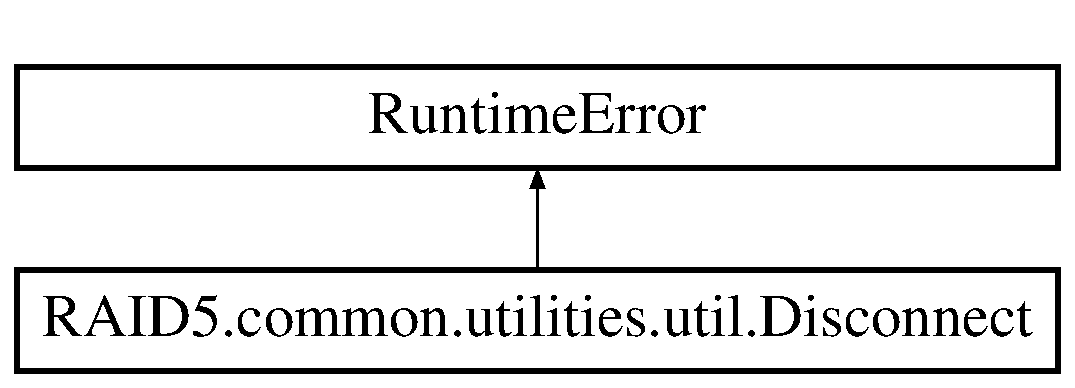
\includegraphics[height=2.000000cm]{class_r_a_i_d5_1_1common_1_1utilities_1_1util_1_1_disconnect}
\end{center}
\end{figure}
\subsection*{Public Member Functions}
\begin{DoxyCompactItemize}
\item 
\mbox{\Hypertarget{class_r_a_i_d5_1_1common_1_1utilities_1_1util_1_1_disconnect_a86ba20eb18586d97c9d4ebefa2b68be1}\label{class_r_a_i_d5_1_1common_1_1utilities_1_1util_1_1_disconnect_a86ba20eb18586d97c9d4ebefa2b68be1}} 
def {\bfseries \+\_\+\+\_\+init\+\_\+\+\_\+} (self, desc=\char`\"{}Disconnect\char`\"{})
\end{DoxyCompactItemize}


The documentation for this class was generated from the following file\+:\begin{DoxyCompactItemize}
\item 
C\+:/cygwin64/tmp/\+R\+A\+I\+D5/common/utilities/util.\+py\end{DoxyCompactItemize}

\hypertarget{class_r_a_i_d5_1_1frontend_1_1services_1_1disconnect__service_1_1_disconnect_service}{}\section{R\+A\+I\+D5.\+frontend.\+services.\+disconnect\+\_\+service.\+Disconnect\+Service Class Reference}
\label{class_r_a_i_d5_1_1frontend_1_1services_1_1disconnect__service_1_1_disconnect_service}\index{R\+A\+I\+D5.\+frontend.\+services.\+disconnect\+\_\+service.\+Disconnect\+Service@{R\+A\+I\+D5.\+frontend.\+services.\+disconnect\+\_\+service.\+Disconnect\+Service}}
Inheritance diagram for R\+A\+I\+D5.\+frontend.\+services.\+disconnect\+\_\+service.\+Disconnect\+Service\+:\begin{figure}[H]
\begin{center}
\leavevmode
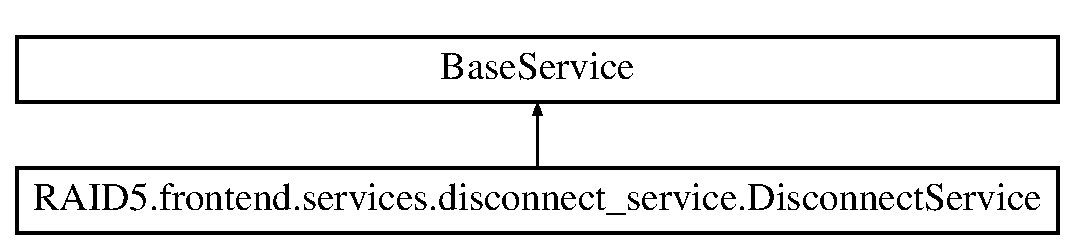
\includegraphics[height=2.000000cm]{class_r_a_i_d5_1_1frontend_1_1services_1_1disconnect__service_1_1_disconnect_service}
\end{center}
\end{figure}
\subsection*{Public Member Functions}
\begin{DoxyCompactItemize}
\item 
\mbox{\Hypertarget{class_r_a_i_d5_1_1frontend_1_1services_1_1disconnect__service_1_1_disconnect_service_a3f7f1670f09d72ef0ea240bd040b3e11}\label{class_r_a_i_d5_1_1frontend_1_1services_1_1disconnect__service_1_1_disconnect_service_a3f7f1670f09d72ef0ea240bd040b3e11}} 
def {\bfseries \+\_\+\+\_\+init\+\_\+\+\_\+} (self, entry, pollables, args)
\item 
\mbox{\Hypertarget{class_r_a_i_d5_1_1frontend_1_1services_1_1disconnect__service_1_1_disconnect_service_abc80e7ca56fe81b034440508285192ca}\label{class_r_a_i_d5_1_1frontend_1_1services_1_1disconnect__service_1_1_disconnect_service_abc80e7ca56fe81b034440508285192ca}} 
def {\bfseries before\+\_\+disconnect} (self, entry)
\item 
\mbox{\Hypertarget{class_r_a_i_d5_1_1frontend_1_1services_1_1disconnect__service_1_1_disconnect_service_abe0279732d686c2f6edc24fdbe9e06ab}\label{class_r_a_i_d5_1_1frontend_1_1services_1_1disconnect__service_1_1_disconnect_service_abe0279732d686c2f6edc24fdbe9e06ab}} 
def {\bfseries after\+\_\+disconnect} (self, entry)
\item 
\mbox{\Hypertarget{class_r_a_i_d5_1_1frontend_1_1services_1_1disconnect__service_1_1_disconnect_service_ac774361849aa7b222401f62dc5eb4947}\label{class_r_a_i_d5_1_1frontend_1_1services_1_1disconnect__service_1_1_disconnect_service_ac774361849aa7b222401f62dc5eb4947}} 
def {\bfseries before\+\_\+response\+\_\+status} (self, entry)
\item 
\mbox{\Hypertarget{class_r_a_i_d5_1_1frontend_1_1services_1_1disconnect__service_1_1_disconnect_service_a01889d0d69632d9fe51514c4fbcbadb0}\label{class_r_a_i_d5_1_1frontend_1_1services_1_1disconnect__service_1_1_disconnect_service_a01889d0d69632d9fe51514c4fbcbadb0}} 
def {\bfseries on\+\_\+finish} (self, entry)
\item 
\mbox{\Hypertarget{class_r_a_i_d5_1_1frontend_1_1services_1_1disconnect__service_1_1_disconnect_service_a5a45909b05865c62e4f77842d8ca436e}\label{class_r_a_i_d5_1_1frontend_1_1services_1_1disconnect__service_1_1_disconnect_service_a5a45909b05865c62e4f77842d8ca436e}} 
def {\bfseries before\+\_\+response\+\_\+headers} (self, entry)
\end{DoxyCompactItemize}
\subsection*{Static Public Member Functions}
\begin{DoxyCompactItemize}
\item 
\mbox{\Hypertarget{class_r_a_i_d5_1_1frontend_1_1services_1_1disconnect__service_1_1_disconnect_service_a402bfda39952547f2bf8350826a359fe}\label{class_r_a_i_d5_1_1frontend_1_1services_1_1disconnect__service_1_1_disconnect_service_a402bfda39952547f2bf8350826a359fe}} 
def {\bfseries get\+\_\+name} ()
\end{DoxyCompactItemize}
\subsection*{Static Public Attributes}
\begin{DoxyCompactItemize}
\item 
list {\bfseries S\+T\+A\+T\+ES}
\end{DoxyCompactItemize}


\subsection{Member Data Documentation}
\mbox{\Hypertarget{class_r_a_i_d5_1_1frontend_1_1services_1_1disconnect__service_1_1_disconnect_service_ac934d9262340d5c3da0a913ac2a6f656}\label{class_r_a_i_d5_1_1frontend_1_1services_1_1disconnect__service_1_1_disconnect_service_ac934d9262340d5c3da0a913ac2a6f656}} 
\index{R\+A\+I\+D5\+::frontend\+::services\+::disconnect\+\_\+service\+::\+Disconnect\+Service@{R\+A\+I\+D5\+::frontend\+::services\+::disconnect\+\_\+service\+::\+Disconnect\+Service}!S\+T\+A\+T\+ES@{S\+T\+A\+T\+ES}}
\index{S\+T\+A\+T\+ES@{S\+T\+A\+T\+ES}!R\+A\+I\+D5\+::frontend\+::services\+::disconnect\+\_\+service\+::\+Disconnect\+Service@{R\+A\+I\+D5\+::frontend\+::services\+::disconnect\+\_\+service\+::\+Disconnect\+Service}}
\subsubsection{\texorpdfstring{S\+T\+A\+T\+ES}{STATES}}
{\footnotesize\ttfamily list R\+A\+I\+D5.\+frontend.\+services.\+disconnect\+\_\+service.\+Disconnect\+Service.\+S\+T\+A\+T\+ES\hspace{0.3cm}{\ttfamily [static]}}

{\bfseries Initial value\+:}
\begin{DoxyCode}
=  [
        \hyperlink{classstate_1_1_state}{state.State}(
            DISCONNECT\_STATE,
            [FINAL\_STATE],
            before\_disconnect,
            after\_disconnect,
        ),
        \hyperlink{classstate_1_1_state}{state.State}(
            FINAL\_STATE,
            [FINAL\_STATE]
        )
    ]
\end{DoxyCode}


The documentation for this class was generated from the following file\+:\begin{DoxyCompactItemize}
\item 
C\+:/cygwin64/tmp/\+R\+A\+I\+D5/frontend/services/disconnect\+\_\+service.\+py\end{DoxyCompactItemize}

\hypertarget{class_r_a_i_d5_1_1frontend_1_1utilities_1_1disk__manager_1_1_disk_manager}{}\section{R\+A\+I\+D5.\+frontend.\+utilities.\+disk\+\_\+manager.\+Disk\+Manager Class Reference}
\label{class_r_a_i_d5_1_1frontend_1_1utilities_1_1disk__manager_1_1_disk_manager}\index{R\+A\+I\+D5.\+frontend.\+utilities.\+disk\+\_\+manager.\+Disk\+Manager@{R\+A\+I\+D5.\+frontend.\+utilities.\+disk\+\_\+manager.\+Disk\+Manager}}
Inheritance diagram for R\+A\+I\+D5.\+frontend.\+utilities.\+disk\+\_\+manager.\+Disk\+Manager\+:\begin{figure}[H]
\begin{center}
\leavevmode
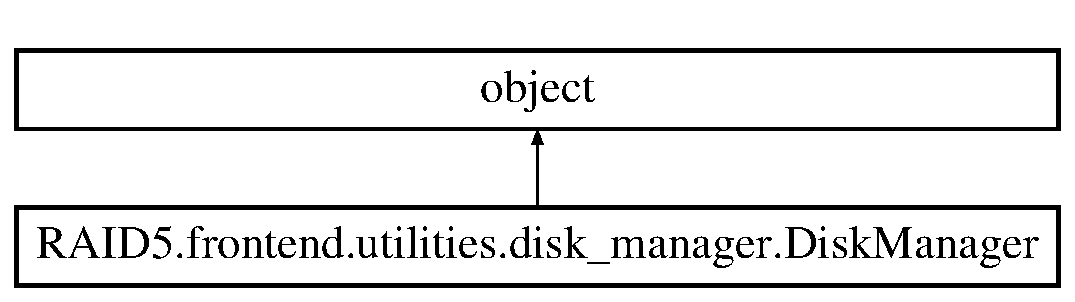
\includegraphics[height=2.000000cm]{class_r_a_i_d5_1_1frontend_1_1utilities_1_1disk__manager_1_1_disk_manager}
\end{center}
\end{figure}
\subsection*{Public Member Functions}
\begin{DoxyCompactItemize}
\item 
\mbox{\Hypertarget{class_r_a_i_d5_1_1frontend_1_1utilities_1_1disk__manager_1_1_disk_manager_aebf7e397d66638593416763f24da1b23}\label{class_r_a_i_d5_1_1frontend_1_1utilities_1_1disk__manager_1_1_disk_manager_aebf7e397d66638593416763f24da1b23}} 
def {\bfseries \+\_\+\+\_\+init\+\_\+\+\_\+} (self, disks, pollables, parent, client\+\_\+contexts)
\item 
\mbox{\Hypertarget{class_r_a_i_d5_1_1frontend_1_1utilities_1_1disk__manager_1_1_disk_manager_a3e1cc950045e74e82c3df387a37a45ae}\label{class_r_a_i_d5_1_1frontend_1_1utilities_1_1disk__manager_1_1_disk_manager_a3e1cc950045e74e82c3df387a37a45ae}} 
def {\bfseries add\+\_\+bds\+\_\+client} (self, parent, client\+\_\+context, client\+\_\+update, pollables)
\item 
\mbox{\Hypertarget{class_r_a_i_d5_1_1frontend_1_1utilities_1_1disk__manager_1_1_disk_manager_a33c98d9dff3816d3f9289ef231fe2f21}\label{class_r_a_i_d5_1_1frontend_1_1utilities_1_1disk__manager_1_1_disk_manager_a33c98d9dff3816d3f9289ef231fe2f21}} 
def {\bfseries get\+\_\+responses} (self)
\item 
\mbox{\Hypertarget{class_r_a_i_d5_1_1frontend_1_1utilities_1_1disk__manager_1_1_disk_manager_a4ea9c35624035aab6f333484505044e6}\label{class_r_a_i_d5_1_1frontend_1_1utilities_1_1disk__manager_1_1_disk_manager_a4ea9c35624035aab6f333484505044e6}} 
def {\bfseries check\+\_\+common\+\_\+status\+\_\+code} (self, common\+\_\+status\+\_\+code)
\item 
\mbox{\Hypertarget{class_r_a_i_d5_1_1frontend_1_1utilities_1_1disk__manager_1_1_disk_manager_a442742d8aa207953583ece1144af1db0}\label{class_r_a_i_d5_1_1frontend_1_1utilities_1_1disk__manager_1_1_disk_manager_a442742d8aa207953583ece1144af1db0}} 
def {\bfseries check\+\_\+if\+\_\+finished} (self)
\end{DoxyCompactItemize}


The documentation for this class was generated from the following file\+:\begin{DoxyCompactItemize}
\item 
C\+:/cygwin64/tmp/\+R\+A\+I\+D5/frontend/utilities/disk\+\_\+manager.\+py\end{DoxyCompactItemize}

\hypertarget{class_r_a_i_d5_1_1common_1_1utilities_1_1util_1_1_disk_refused}{}\section{R\+A\+I\+D5.\+common.\+utilities.\+util.\+Disk\+Refused Class Reference}
\label{class_r_a_i_d5_1_1common_1_1utilities_1_1util_1_1_disk_refused}\index{R\+A\+I\+D5.\+common.\+utilities.\+util.\+Disk\+Refused@{R\+A\+I\+D5.\+common.\+utilities.\+util.\+Disk\+Refused}}
Inheritance diagram for R\+A\+I\+D5.\+common.\+utilities.\+util.\+Disk\+Refused\+:\begin{figure}[H]
\begin{center}
\leavevmode
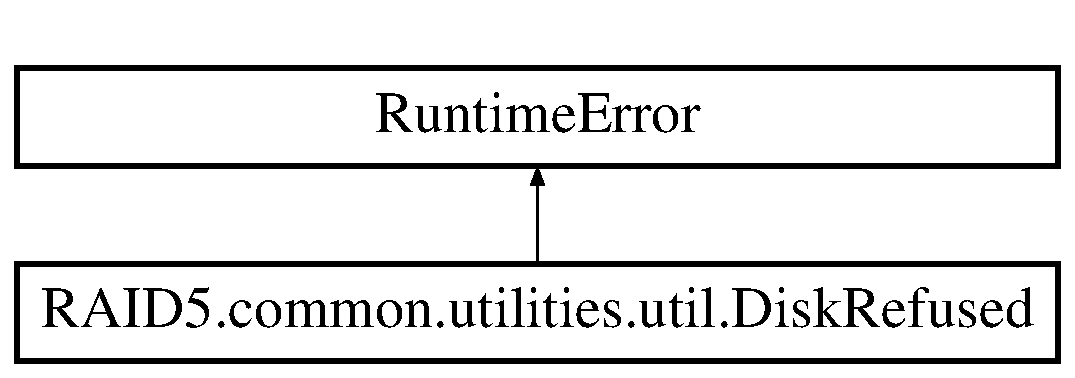
\includegraphics[height=2.000000cm]{class_r_a_i_d5_1_1common_1_1utilities_1_1util_1_1_disk_refused}
\end{center}
\end{figure}
\subsection*{Public Member Functions}
\begin{DoxyCompactItemize}
\item 
\mbox{\Hypertarget{class_r_a_i_d5_1_1common_1_1utilities_1_1util_1_1_disk_refused_ac5eb59596d5f7689eb3c8bd8b4158c3c}\label{class_r_a_i_d5_1_1common_1_1utilities_1_1util_1_1_disk_refused_ac5eb59596d5f7689eb3c8bd8b4158c3c}} 
def {\bfseries \+\_\+\+\_\+init\+\_\+\+\_\+} (self, disk\+\_\+\+U\+U\+ID, desc=\char`\"{}Disk Refused to connect\char`\"{})
\item 
\mbox{\Hypertarget{class_r_a_i_d5_1_1common_1_1utilities_1_1util_1_1_disk_refused_ab08b8f739c377d8651c0a22c8dd554b9}\label{class_r_a_i_d5_1_1common_1_1utilities_1_1util_1_1_disk_refused_ab08b8f739c377d8651c0a22c8dd554b9}} 
def {\bfseries disk\+\_\+\+U\+U\+ID} (self)
\end{DoxyCompactItemize}


The documentation for this class was generated from the following file\+:\begin{DoxyCompactItemize}
\item 
C\+:/cygwin64/tmp/\+R\+A\+I\+D5/common/utilities/util.\+py\end{DoxyCompactItemize}

\hypertarget{class_r_a_i_d5_1_1frontend_1_1services_1_1display__disks__service_1_1_display_disks_service}{}\section{R\+A\+I\+D5.\+frontend.\+services.\+display\+\_\+disks\+\_\+service.\+Display\+Disks\+Service Class Reference}
\label{class_r_a_i_d5_1_1frontend_1_1services_1_1display__disks__service_1_1_display_disks_service}\index{R\+A\+I\+D5.\+frontend.\+services.\+display\+\_\+disks\+\_\+service.\+Display\+Disks\+Service@{R\+A\+I\+D5.\+frontend.\+services.\+display\+\_\+disks\+\_\+service.\+Display\+Disks\+Service}}
Inheritance diagram for R\+A\+I\+D5.\+frontend.\+services.\+display\+\_\+disks\+\_\+service.\+Display\+Disks\+Service\+:\begin{figure}[H]
\begin{center}
\leavevmode
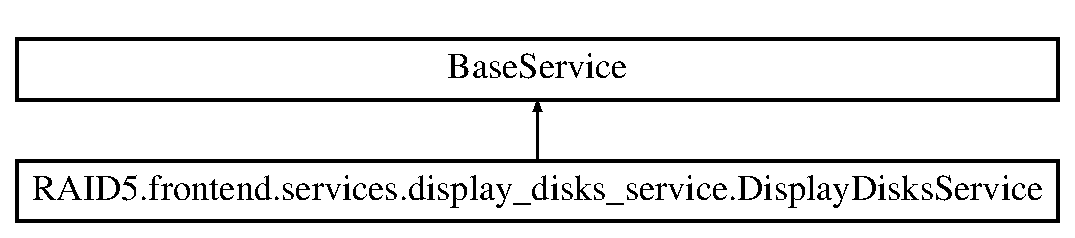
\includegraphics[height=2.000000cm]{class_r_a_i_d5_1_1frontend_1_1services_1_1display__disks__service_1_1_display_disks_service}
\end{center}
\end{figure}
\subsection*{Public Member Functions}
\begin{DoxyCompactItemize}
\item 
\mbox{\Hypertarget{class_r_a_i_d5_1_1frontend_1_1services_1_1display__disks__service_1_1_display_disks_service_a1e7c2fb442f4fef408fc50fd15affbc6}\label{class_r_a_i_d5_1_1frontend_1_1services_1_1display__disks__service_1_1_display_disks_service_a1e7c2fb442f4fef408fc50fd15affbc6}} 
def {\bfseries \+\_\+\+\_\+init\+\_\+\+\_\+} (self, entry, pollables, args)
\item 
\mbox{\Hypertarget{class_r_a_i_d5_1_1frontend_1_1services_1_1display__disks__service_1_1_display_disks_service_a1a2fcd40542c99bb39aec33aa4fd2895}\label{class_r_a_i_d5_1_1frontend_1_1services_1_1display__disks__service_1_1_display_disks_service_a1a2fcd40542c99bb39aec33aa4fd2895}} 
def {\bfseries before\+\_\+response\+\_\+status} (self, entry)
\item 
\mbox{\Hypertarget{class_r_a_i_d5_1_1frontend_1_1services_1_1display__disks__service_1_1_display_disks_service_ab858414cf065474f9ed5b24bcc376b28}\label{class_r_a_i_d5_1_1frontend_1_1services_1_1display__disks__service_1_1_display_disks_service_ab858414cf065474f9ed5b24bcc376b28}} 
def {\bfseries before\+\_\+response\+\_\+headers} (self, entry)
\end{DoxyCompactItemize}
\subsection*{Static Public Member Functions}
\begin{DoxyCompactItemize}
\item 
\mbox{\Hypertarget{class_r_a_i_d5_1_1frontend_1_1services_1_1display__disks__service_1_1_display_disks_service_a9c193a3f90fa22c4b1cc465608e0e7ec}\label{class_r_a_i_d5_1_1frontend_1_1services_1_1display__disks__service_1_1_display_disks_service_a9c193a3f90fa22c4b1cc465608e0e7ec}} 
def {\bfseries get\+\_\+name} ()
\end{DoxyCompactItemize}


The documentation for this class was generated from the following file\+:\begin{DoxyCompactItemize}
\item 
C\+:/cygwin64/tmp/\+R\+A\+I\+D5/frontend/services/display\+\_\+disks\+\_\+service.\+py\end{DoxyCompactItemize}

\hypertarget{class_r_a_i_d5_1_1common_1_1services_1_1form__service_1_1_file_form_service}{}\section{R\+A\+I\+D5.\+common.\+services.\+form\+\_\+service.\+File\+Form\+Service Class Reference}
\label{class_r_a_i_d5_1_1common_1_1services_1_1form__service_1_1_file_form_service}\index{R\+A\+I\+D5.\+common.\+services.\+form\+\_\+service.\+File\+Form\+Service@{R\+A\+I\+D5.\+common.\+services.\+form\+\_\+service.\+File\+Form\+Service}}
Inheritance diagram for R\+A\+I\+D5.\+common.\+services.\+form\+\_\+service.\+File\+Form\+Service\+:\begin{figure}[H]
\begin{center}
\leavevmode
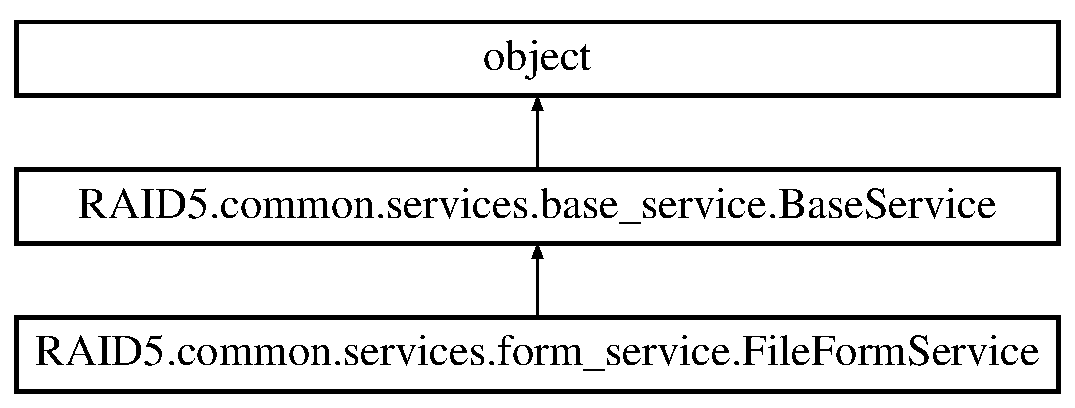
\includegraphics[height=3.000000cm]{class_r_a_i_d5_1_1common_1_1services_1_1form__service_1_1_file_form_service}
\end{center}
\end{figure}
\subsection*{Public Member Functions}
\begin{DoxyCompactItemize}
\item 
\mbox{\Hypertarget{class_r_a_i_d5_1_1common_1_1services_1_1form__service_1_1_file_form_service_a7cae473594b522f010be41c8143ee8c1}\label{class_r_a_i_d5_1_1common_1_1services_1_1form__service_1_1_file_form_service_a7cae473594b522f010be41c8143ee8c1}} 
def {\bfseries \+\_\+\+\_\+init\+\_\+\+\_\+} (self, entry, pollables, args)
\item 
\mbox{\Hypertarget{class_r_a_i_d5_1_1common_1_1services_1_1form__service_1_1_file_form_service_a5e35e9c35ee9356c6c2fa7288ad58c25}\label{class_r_a_i_d5_1_1common_1_1services_1_1form__service_1_1_file_form_service_a5e35e9c35ee9356c6c2fa7288ad58c25}} 
def {\bfseries after\+\_\+start} (self, entry)
\item 
\mbox{\Hypertarget{class_r_a_i_d5_1_1common_1_1services_1_1form__service_1_1_file_form_service_abcbe805b5294b0a393bfe358ab77c5c6}\label{class_r_a_i_d5_1_1common_1_1services_1_1form__service_1_1_file_form_service_abcbe805b5294b0a393bfe358ab77c5c6}} 
def {\bfseries after\+\_\+headers} (self, entry)
\item 
\mbox{\Hypertarget{class_r_a_i_d5_1_1common_1_1services_1_1form__service_1_1_file_form_service_acf294d2c5cac14fc6a7f85f05fb28d14}\label{class_r_a_i_d5_1_1common_1_1services_1_1form__service_1_1_file_form_service_acf294d2c5cac14fc6a7f85f05fb28d14}} 
def {\bfseries after\+\_\+content} (self, entry)
\item 
\mbox{\Hypertarget{class_r_a_i_d5_1_1common_1_1services_1_1form__service_1_1_file_form_service_a2dd48fe54b066574dd1a7ab441f3a188}\label{class_r_a_i_d5_1_1common_1_1services_1_1form__service_1_1_file_form_service_a2dd48fe54b066574dd1a7ab441f3a188}} 
def {\bfseries before\+\_\+content} (self, entry)
\item 
\mbox{\Hypertarget{class_r_a_i_d5_1_1common_1_1services_1_1form__service_1_1_file_form_service_a162ea4f96c74554d350b4f9123793ded}\label{class_r_a_i_d5_1_1common_1_1services_1_1form__service_1_1_file_form_service_a162ea4f96c74554d350b4f9123793ded}} 
def {\bfseries handle\+\_\+content} (self, entry, content)
\item 
\mbox{\Hypertarget{class_r_a_i_d5_1_1common_1_1services_1_1form__service_1_1_file_form_service_a4c335209589b3961e1b813cc54ead899}\label{class_r_a_i_d5_1_1common_1_1services_1_1form__service_1_1_file_form_service_a4c335209589b3961e1b813cc54ead899}} 
def {\bfseries before\+\_\+response\+\_\+headers} (self, entry)
\item 
\mbox{\Hypertarget{class_r_a_i_d5_1_1common_1_1services_1_1form__service_1_1_file_form_service_a46211cc9ccaede54578f17b02e9493ff}\label{class_r_a_i_d5_1_1common_1_1services_1_1form__service_1_1_file_form_service_a46211cc9ccaede54578f17b02e9493ff}} 
def {\bfseries arg\+\_\+handle} (self, arg, next\+\_\+state)
\item 
\mbox{\Hypertarget{class_r_a_i_d5_1_1common_1_1services_1_1form__service_1_1_file_form_service_a2c5a8072bcbb001432a90afd81db42c3}\label{class_r_a_i_d5_1_1common_1_1services_1_1form__service_1_1_file_form_service_a2c5a8072bcbb001432a90afd81db42c3}} 
def {\bfseries file\+\_\+handle} (self, buf, next\+\_\+state)
\end{DoxyCompactItemize}
\subsection*{Static Public Member Functions}
\begin{DoxyCompactItemize}
\item 
\mbox{\Hypertarget{class_r_a_i_d5_1_1common_1_1services_1_1form__service_1_1_file_form_service_a8392d7038cfb99930294b170a34d10cb}\label{class_r_a_i_d5_1_1common_1_1services_1_1form__service_1_1_file_form_service_a8392d7038cfb99930294b170a34d10cb}} 
def {\bfseries get\+\_\+name} ()
\end{DoxyCompactItemize}
\subsection*{Static Public Attributes}
\begin{DoxyCompactItemize}
\item 
list {\bfseries S\+T\+A\+T\+ES}
\end{DoxyCompactItemize}


\subsection{Member Data Documentation}
\mbox{\Hypertarget{class_r_a_i_d5_1_1common_1_1services_1_1form__service_1_1_file_form_service_a41a5dfe1b65d48a709f13d6e23f08f3a}\label{class_r_a_i_d5_1_1common_1_1services_1_1form__service_1_1_file_form_service_a41a5dfe1b65d48a709f13d6e23f08f3a}} 
\index{R\+A\+I\+D5\+::common\+::services\+::form\+\_\+service\+::\+File\+Form\+Service@{R\+A\+I\+D5\+::common\+::services\+::form\+\_\+service\+::\+File\+Form\+Service}!S\+T\+A\+T\+ES@{S\+T\+A\+T\+ES}}
\index{S\+T\+A\+T\+ES@{S\+T\+A\+T\+ES}!R\+A\+I\+D5\+::common\+::services\+::form\+\_\+service\+::\+File\+Form\+Service@{R\+A\+I\+D5\+::common\+::services\+::form\+\_\+service\+::\+File\+Form\+Service}}
\subsubsection{\texorpdfstring{S\+T\+A\+T\+ES}{STATES}}
{\footnotesize\ttfamily list R\+A\+I\+D5.\+common.\+services.\+form\+\_\+service.\+File\+Form\+Service.\+S\+T\+A\+T\+ES\hspace{0.3cm}{\ttfamily [static]}}

{\bfseries Initial value\+:}
\begin{DoxyCode}
=  [
        \hyperlink{classstate_1_1_state}{state.State}(
            START\_STATE,
            [HEADERS\_STATE],
            after\_func=after\_start,
        ),
        \hyperlink{classstate_1_1_state}{state.State}(
            HEADERS\_STATE,
            [CONTENT\_STATE],
            after\_func=after\_headers
        ),
        \hyperlink{classstate_1_1_state}{state.State}(
            CONTENT\_STATE,
            [HEADERS\_STATE, FINAL\_STATE],
            after\_func=after\_content
        ),
        \hyperlink{classstate_1_1_state}{state.State}(
            FINAL\_STATE,
            [FINAL\_STATE]
        )
    ]
\end{DoxyCode}


The documentation for this class was generated from the following file\+:\begin{DoxyCompactItemize}
\item 
C\+:/cygwin64/tmp/\+R\+A\+I\+D5/common/services/form\+\_\+service.\+py\end{DoxyCompactItemize}

\hypertarget{class_r_a_i_d5_1_1block__device_1_1services_1_1get__block__service_1_1_get_block_service}{}\section{R\+A\+I\+D5.\+block\+\_\+device.\+services.\+get\+\_\+block\+\_\+service.\+Get\+Block\+Service Class Reference}
\label{class_r_a_i_d5_1_1block__device_1_1services_1_1get__block__service_1_1_get_block_service}\index{R\+A\+I\+D5.\+block\+\_\+device.\+services.\+get\+\_\+block\+\_\+service.\+Get\+Block\+Service@{R\+A\+I\+D5.\+block\+\_\+device.\+services.\+get\+\_\+block\+\_\+service.\+Get\+Block\+Service}}


A Block Device Service that allows the Frontend Server to request a block.  


Inheritance diagram for R\+A\+I\+D5.\+block\+\_\+device.\+services.\+get\+\_\+block\+\_\+service.\+Get\+Block\+Service\+:\begin{figure}[H]
\begin{center}
\leavevmode
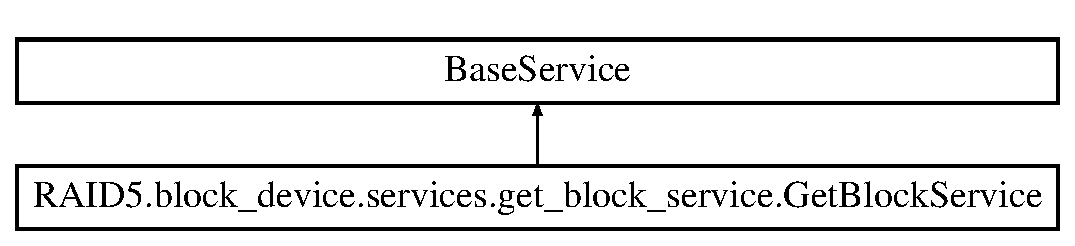
\includegraphics[height=2.000000cm]{class_r_a_i_d5_1_1block__device_1_1services_1_1get__block__service_1_1_get_block_service}
\end{center}
\end{figure}
\subsection*{Public Member Functions}
\begin{DoxyCompactItemize}
\item 
def \hyperlink{class_r_a_i_d5_1_1block__device_1_1services_1_1get__block__service_1_1_get_block_service_a6fe680bf73350c7bdb9f97266b6fa6ca}{\+\_\+\+\_\+init\+\_\+\+\_\+} (self, entry, pollables, args)
\begin{DoxyCompactList}\small\item\em Constructor for \hyperlink{class_r_a_i_d5_1_1block__device_1_1services_1_1get__block__service_1_1_get_block_service}{Get\+Block\+Service}. \end{DoxyCompactList}\item 
def \hyperlink{class_r_a_i_d5_1_1block__device_1_1services_1_1get__block__service_1_1_get_block_service_a15bbebfff6a6da5eb532ecb8a94cefa6}{before\+\_\+response\+\_\+status} (self, entry)
\begin{DoxyCompactList}\small\item\em What the service does before sending a response status see \hyperlink{class_r_a_i_d5_1_1common_1_1services_1_1base__service_1_1_base_service}{common.\+services.\+base\+\_\+service.\+Base\+Service} function reads the block requested from the disk file. \end{DoxyCompactList}\item 
\mbox{\Hypertarget{class_r_a_i_d5_1_1block__device_1_1services_1_1get__block__service_1_1_get_block_service_a287839bc5348ebbf7e959b10f27c1930}\label{class_r_a_i_d5_1_1block__device_1_1services_1_1get__block__service_1_1_get_block_service_a287839bc5348ebbf7e959b10f27c1930}} 
def \hyperlink{class_r_a_i_d5_1_1block__device_1_1services_1_1get__block__service_1_1_get_block_service_a287839bc5348ebbf7e959b10f27c1930}{before\+\_\+terminate} (self, entry)
\begin{DoxyCompactList}\small\item\em What the service needs to do before terminating see \hyperlink{class_r_a_i_d5_1_1common_1_1services_1_1base__service_1_1_base_service}{common.\+services.\+base\+\_\+service.\+Base\+Service} closes the disk file descriptor. \end{DoxyCompactList}\end{DoxyCompactItemize}
\subsection*{Static Public Member Functions}
\begin{DoxyCompactItemize}
\item 
def \hyperlink{class_r_a_i_d5_1_1block__device_1_1services_1_1get__block__service_1_1_get_block_service_a813d2b4bd5bc7a7fea09475792396db2}{get\+\_\+name} ()
\begin{DoxyCompactList}\small\item\em Name of the service needed for Frontend purposes, creating clients required by \hyperlink{class_r_a_i_d5_1_1common_1_1services_1_1base__service_1_1_base_service}{common.\+services.\+base\+\_\+service.\+Base\+Service}. \end{DoxyCompactList}\end{DoxyCompactItemize}


\subsection{Detailed Description}
A Block Device Service that allows the Frontend Server to request a block. 

\subsection{Constructor \& Destructor Documentation}
\mbox{\Hypertarget{class_r_a_i_d5_1_1block__device_1_1services_1_1get__block__service_1_1_get_block_service_a6fe680bf73350c7bdb9f97266b6fa6ca}\label{class_r_a_i_d5_1_1block__device_1_1services_1_1get__block__service_1_1_get_block_service_a6fe680bf73350c7bdb9f97266b6fa6ca}} 
\index{R\+A\+I\+D5\+::block\+\_\+device\+::services\+::get\+\_\+block\+\_\+service\+::\+Get\+Block\+Service@{R\+A\+I\+D5\+::block\+\_\+device\+::services\+::get\+\_\+block\+\_\+service\+::\+Get\+Block\+Service}!\+\_\+\+\_\+init\+\_\+\+\_\+@{\+\_\+\+\_\+init\+\_\+\+\_\+}}
\index{\+\_\+\+\_\+init\+\_\+\+\_\+@{\+\_\+\+\_\+init\+\_\+\+\_\+}!R\+A\+I\+D5\+::block\+\_\+device\+::services\+::get\+\_\+block\+\_\+service\+::\+Get\+Block\+Service@{R\+A\+I\+D5\+::block\+\_\+device\+::services\+::get\+\_\+block\+\_\+service\+::\+Get\+Block\+Service}}
\subsubsection{\texorpdfstring{\+\_\+\+\_\+init\+\_\+\+\_\+()}{\_\_init\_\_()}}
{\footnotesize\ttfamily def R\+A\+I\+D5.\+block\+\_\+device.\+services.\+get\+\_\+block\+\_\+service.\+Get\+Block\+Service.\+\_\+\+\_\+init\+\_\+\+\_\+ (\begin{DoxyParamCaption}\item[{}]{self,  }\item[{}]{entry,  }\item[{}]{pollables,  }\item[{}]{args }\end{DoxyParamCaption})}



Constructor for \hyperlink{class_r_a_i_d5_1_1block__device_1_1services_1_1get__block__service_1_1_get_block_service}{Get\+Block\+Service}. 


\begin{DoxyParams}{Parameters}
{\em entry} & (pollable) the entry (probably common.\+pollables.\+service\+\_\+socket) using the service \\
\hline
{\em pollables} & (dict) All the pollables currently in the server \\
\hline
{\em args} & (dict) Arguments for this service \\
\hline
\end{DoxyParams}


\subsection{Member Function Documentation}
\mbox{\Hypertarget{class_r_a_i_d5_1_1block__device_1_1services_1_1get__block__service_1_1_get_block_service_a15bbebfff6a6da5eb532ecb8a94cefa6}\label{class_r_a_i_d5_1_1block__device_1_1services_1_1get__block__service_1_1_get_block_service_a15bbebfff6a6da5eb532ecb8a94cefa6}} 
\index{R\+A\+I\+D5\+::block\+\_\+device\+::services\+::get\+\_\+block\+\_\+service\+::\+Get\+Block\+Service@{R\+A\+I\+D5\+::block\+\_\+device\+::services\+::get\+\_\+block\+\_\+service\+::\+Get\+Block\+Service}!before\+\_\+response\+\_\+status@{before\+\_\+response\+\_\+status}}
\index{before\+\_\+response\+\_\+status@{before\+\_\+response\+\_\+status}!R\+A\+I\+D5\+::block\+\_\+device\+::services\+::get\+\_\+block\+\_\+service\+::\+Get\+Block\+Service@{R\+A\+I\+D5\+::block\+\_\+device\+::services\+::get\+\_\+block\+\_\+service\+::\+Get\+Block\+Service}}
\subsubsection{\texorpdfstring{before\+\_\+response\+\_\+status()}{before\_response\_status()}}
{\footnotesize\ttfamily def R\+A\+I\+D5.\+block\+\_\+device.\+services.\+get\+\_\+block\+\_\+service.\+Get\+Block\+Service.\+before\+\_\+response\+\_\+status (\begin{DoxyParamCaption}\item[{}]{self,  }\item[{}]{entry }\end{DoxyParamCaption})}



What the service does before sending a response status see \hyperlink{class_r_a_i_d5_1_1common_1_1services_1_1base__service_1_1_base_service}{common.\+services.\+base\+\_\+service.\+Base\+Service} function reads the block requested from the disk file. 


\begin{DoxyParams}{Parameters}
{\em entry} & (pollable) the entry that the service is assigned to \\
\hline
\end{DoxyParams}
\begin{DoxyReturn}{Returns}
(bool) if finished and ready to move on 
\end{DoxyReturn}
\mbox{\Hypertarget{class_r_a_i_d5_1_1block__device_1_1services_1_1get__block__service_1_1_get_block_service_a813d2b4bd5bc7a7fea09475792396db2}\label{class_r_a_i_d5_1_1block__device_1_1services_1_1get__block__service_1_1_get_block_service_a813d2b4bd5bc7a7fea09475792396db2}} 
\index{R\+A\+I\+D5\+::block\+\_\+device\+::services\+::get\+\_\+block\+\_\+service\+::\+Get\+Block\+Service@{R\+A\+I\+D5\+::block\+\_\+device\+::services\+::get\+\_\+block\+\_\+service\+::\+Get\+Block\+Service}!get\+\_\+name@{get\+\_\+name}}
\index{get\+\_\+name@{get\+\_\+name}!R\+A\+I\+D5\+::block\+\_\+device\+::services\+::get\+\_\+block\+\_\+service\+::\+Get\+Block\+Service@{R\+A\+I\+D5\+::block\+\_\+device\+::services\+::get\+\_\+block\+\_\+service\+::\+Get\+Block\+Service}}
\subsubsection{\texorpdfstring{get\+\_\+name()}{get\_name()}}
{\footnotesize\ttfamily def R\+A\+I\+D5.\+block\+\_\+device.\+services.\+get\+\_\+block\+\_\+service.\+Get\+Block\+Service.\+get\+\_\+name (\begin{DoxyParamCaption}{ }\end{DoxyParamCaption})\hspace{0.3cm}{\ttfamily [static]}}



Name of the service needed for Frontend purposes, creating clients required by \hyperlink{class_r_a_i_d5_1_1common_1_1services_1_1base__service_1_1_base_service}{common.\+services.\+base\+\_\+service.\+Base\+Service}. 

\begin{DoxyReturn}{Returns}
(str) service name 
\end{DoxyReturn}


The documentation for this class was generated from the following file\+:\begin{DoxyCompactItemize}
\item 
C\+:/cygwin64/tmp/\+R\+A\+I\+D5/block\+\_\+device/services/get\+\_\+block\+\_\+service.\+py\end{DoxyCompactItemize}

\hypertarget{class_r_a_i_d5_1_1block__device_1_1services_1_1get__disk__info__service_1_1_get_disk_info_service}{}\section{R\+A\+I\+D5.\+block\+\_\+device.\+services.\+get\+\_\+disk\+\_\+info\+\_\+service.\+Get\+Disk\+Info\+Service Class Reference}
\label{class_r_a_i_d5_1_1block__device_1_1services_1_1get__disk__info__service_1_1_get_disk_info_service}\index{R\+A\+I\+D5.\+block\+\_\+device.\+services.\+get\+\_\+disk\+\_\+info\+\_\+service.\+Get\+Disk\+Info\+Service@{R\+A\+I\+D5.\+block\+\_\+device.\+services.\+get\+\_\+disk\+\_\+info\+\_\+service.\+Get\+Disk\+Info\+Service}}


A Block Device Service that sends the Frontend it\textquotesingle{}s disk info (block -\/1) Very simple class, just sets the disk\+\_\+info location and then regular \hyperlink{class_r_a_i_d5_1_1common_1_1services_1_1get__file__service_1_1_get_file_service}{common.\+services.\+get\+\_\+file\+\_\+service.\+Get\+File\+Service}.  


Inheritance diagram for R\+A\+I\+D5.\+block\+\_\+device.\+services.\+get\+\_\+disk\+\_\+info\+\_\+service.\+Get\+Disk\+Info\+Service\+:\begin{figure}[H]
\begin{center}
\leavevmode
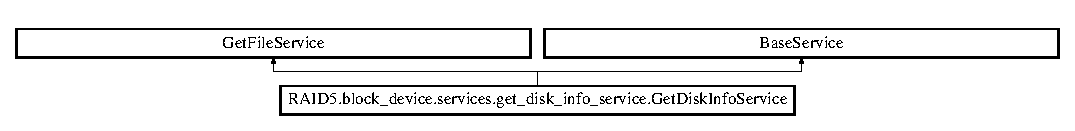
\includegraphics[height=1.314554cm]{class_r_a_i_d5_1_1block__device_1_1services_1_1get__disk__info__service_1_1_get_disk_info_service}
\end{center}
\end{figure}
\subsection*{Public Member Functions}
\begin{DoxyCompactItemize}
\item 
def \hyperlink{class_r_a_i_d5_1_1block__device_1_1services_1_1get__disk__info__service_1_1_get_disk_info_service_a24750dbde71ba0f0c2048e38e64258fa}{\+\_\+\+\_\+init\+\_\+\+\_\+} (self, entry, pollables, args)
\begin{DoxyCompactList}\small\item\em Constructor for \hyperlink{class_r_a_i_d5_1_1block__device_1_1services_1_1get__disk__info__service_1_1_get_disk_info_service}{Get\+Disk\+Info\+Service}. \end{DoxyCompactList}\end{DoxyCompactItemize}
\subsection*{Static Public Member Functions}
\begin{DoxyCompactItemize}
\item 
def \hyperlink{class_r_a_i_d5_1_1block__device_1_1services_1_1get__disk__info__service_1_1_get_disk_info_service_acdcf11106f83ada86ec5a72c0eb8b938}{get\+\_\+name} ()
\begin{DoxyCompactList}\small\item\em Name of the service needed for Frontend purposes, creating clients required by \hyperlink{class_r_a_i_d5_1_1common_1_1services_1_1base__service_1_1_base_service}{common.\+services.\+base\+\_\+service.\+Base\+Service}. \end{DoxyCompactList}\end{DoxyCompactItemize}


\subsection{Detailed Description}
A Block Device Service that sends the Frontend it\textquotesingle{}s disk info (block -\/1) Very simple class, just sets the disk\+\_\+info location and then regular \hyperlink{class_r_a_i_d5_1_1common_1_1services_1_1get__file__service_1_1_get_file_service}{common.\+services.\+get\+\_\+file\+\_\+service.\+Get\+File\+Service}. 

\subsection{Constructor \& Destructor Documentation}
\mbox{\Hypertarget{class_r_a_i_d5_1_1block__device_1_1services_1_1get__disk__info__service_1_1_get_disk_info_service_a24750dbde71ba0f0c2048e38e64258fa}\label{class_r_a_i_d5_1_1block__device_1_1services_1_1get__disk__info__service_1_1_get_disk_info_service_a24750dbde71ba0f0c2048e38e64258fa}} 
\index{R\+A\+I\+D5\+::block\+\_\+device\+::services\+::get\+\_\+disk\+\_\+info\+\_\+service\+::\+Get\+Disk\+Info\+Service@{R\+A\+I\+D5\+::block\+\_\+device\+::services\+::get\+\_\+disk\+\_\+info\+\_\+service\+::\+Get\+Disk\+Info\+Service}!\+\_\+\+\_\+init\+\_\+\+\_\+@{\+\_\+\+\_\+init\+\_\+\+\_\+}}
\index{\+\_\+\+\_\+init\+\_\+\+\_\+@{\+\_\+\+\_\+init\+\_\+\+\_\+}!R\+A\+I\+D5\+::block\+\_\+device\+::services\+::get\+\_\+disk\+\_\+info\+\_\+service\+::\+Get\+Disk\+Info\+Service@{R\+A\+I\+D5\+::block\+\_\+device\+::services\+::get\+\_\+disk\+\_\+info\+\_\+service\+::\+Get\+Disk\+Info\+Service}}
\subsubsection{\texorpdfstring{\+\_\+\+\_\+init\+\_\+\+\_\+()}{\_\_init\_\_()}}
{\footnotesize\ttfamily def R\+A\+I\+D5.\+block\+\_\+device.\+services.\+get\+\_\+disk\+\_\+info\+\_\+service.\+Get\+Disk\+Info\+Service.\+\_\+\+\_\+init\+\_\+\+\_\+ (\begin{DoxyParamCaption}\item[{}]{self,  }\item[{}]{entry,  }\item[{}]{pollables,  }\item[{}]{args }\end{DoxyParamCaption})}



Constructor for \hyperlink{class_r_a_i_d5_1_1block__device_1_1services_1_1get__disk__info__service_1_1_get_disk_info_service}{Get\+Disk\+Info\+Service}. 


\begin{DoxyParams}{Parameters}
{\em entry} & (pollable) the entry (probably common.\+pollables.\+service\+\_\+socket) using the service \\
\hline
{\em pollables} & (dict) All the pollables currently in the server \\
\hline
{\em args} & (dict) Arguments for this service \\
\hline
\end{DoxyParams}


\subsection{Member Function Documentation}
\mbox{\Hypertarget{class_r_a_i_d5_1_1block__device_1_1services_1_1get__disk__info__service_1_1_get_disk_info_service_acdcf11106f83ada86ec5a72c0eb8b938}\label{class_r_a_i_d5_1_1block__device_1_1services_1_1get__disk__info__service_1_1_get_disk_info_service_acdcf11106f83ada86ec5a72c0eb8b938}} 
\index{R\+A\+I\+D5\+::block\+\_\+device\+::services\+::get\+\_\+disk\+\_\+info\+\_\+service\+::\+Get\+Disk\+Info\+Service@{R\+A\+I\+D5\+::block\+\_\+device\+::services\+::get\+\_\+disk\+\_\+info\+\_\+service\+::\+Get\+Disk\+Info\+Service}!get\+\_\+name@{get\+\_\+name}}
\index{get\+\_\+name@{get\+\_\+name}!R\+A\+I\+D5\+::block\+\_\+device\+::services\+::get\+\_\+disk\+\_\+info\+\_\+service\+::\+Get\+Disk\+Info\+Service@{R\+A\+I\+D5\+::block\+\_\+device\+::services\+::get\+\_\+disk\+\_\+info\+\_\+service\+::\+Get\+Disk\+Info\+Service}}
\subsubsection{\texorpdfstring{get\+\_\+name()}{get\_name()}}
{\footnotesize\ttfamily def R\+A\+I\+D5.\+block\+\_\+device.\+services.\+get\+\_\+disk\+\_\+info\+\_\+service.\+Get\+Disk\+Info\+Service.\+get\+\_\+name (\begin{DoxyParamCaption}{ }\end{DoxyParamCaption})\hspace{0.3cm}{\ttfamily [static]}}



Name of the service needed for Frontend purposes, creating clients required by \hyperlink{class_r_a_i_d5_1_1common_1_1services_1_1base__service_1_1_base_service}{common.\+services.\+base\+\_\+service.\+Base\+Service}. 

\begin{DoxyReturn}{Returns}
(str) service name 
\end{DoxyReturn}


The documentation for this class was generated from the following file\+:\begin{DoxyCompactItemize}
\item 
C\+:/cygwin64/tmp/\+R\+A\+I\+D5/block\+\_\+device/services/get\+\_\+disk\+\_\+info\+\_\+service.\+py\end{DoxyCompactItemize}

\hypertarget{class_r_a_i_d5_1_1common_1_1services_1_1get__file__service_1_1_get_file_service}{}\section{R\+A\+I\+D5.\+common.\+services.\+get\+\_\+file\+\_\+service.\+Get\+File\+Service Class Reference}
\label{class_r_a_i_d5_1_1common_1_1services_1_1get__file__service_1_1_get_file_service}\index{R\+A\+I\+D5.\+common.\+services.\+get\+\_\+file\+\_\+service.\+Get\+File\+Service@{R\+A\+I\+D5.\+common.\+services.\+get\+\_\+file\+\_\+service.\+Get\+File\+Service}}
Inheritance diagram for R\+A\+I\+D5.\+common.\+services.\+get\+\_\+file\+\_\+service.\+Get\+File\+Service\+:\begin{figure}[H]
\begin{center}
\leavevmode
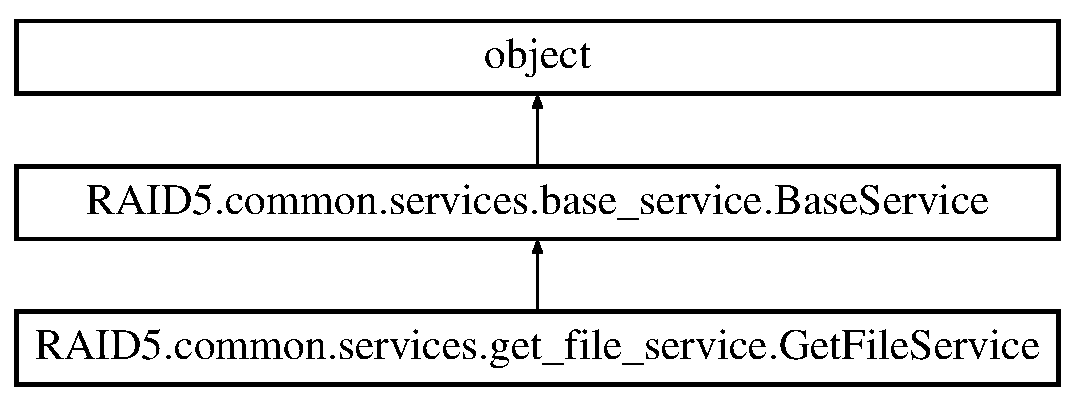
\includegraphics[height=3.000000cm]{class_r_a_i_d5_1_1common_1_1services_1_1get__file__service_1_1_get_file_service}
\end{center}
\end{figure}
\subsection*{Public Member Functions}
\begin{DoxyCompactItemize}
\item 
\mbox{\Hypertarget{class_r_a_i_d5_1_1common_1_1services_1_1get__file__service_1_1_get_file_service_a9011d4d97acc336a3fdd7b44c34abaa5}\label{class_r_a_i_d5_1_1common_1_1services_1_1get__file__service_1_1_get_file_service_a9011d4d97acc336a3fdd7b44c34abaa5}} 
def {\bfseries \+\_\+\+\_\+init\+\_\+\+\_\+} (self, entry, filename)
\item 
\mbox{\Hypertarget{class_r_a_i_d5_1_1common_1_1services_1_1get__file__service_1_1_get_file_service_af9e40a37b80855d4890068c477b51d24}\label{class_r_a_i_d5_1_1common_1_1services_1_1get__file__service_1_1_get_file_service_af9e40a37b80855d4890068c477b51d24}} 
def {\bfseries before\+\_\+response\+\_\+status} (self, entry)
\item 
\mbox{\Hypertarget{class_r_a_i_d5_1_1common_1_1services_1_1get__file__service_1_1_get_file_service_a3ef48982c21b7aeb08722458d0708554}\label{class_r_a_i_d5_1_1common_1_1services_1_1get__file__service_1_1_get_file_service_a3ef48982c21b7aeb08722458d0708554}} 
def {\bfseries before\+\_\+response\+\_\+content} (self, entry, max\+\_\+buffer=constants.\+B\+L\+O\+C\+K\+\_\+\+S\+I\+ZE)
\end{DoxyCompactItemize}
\subsection*{Static Public Member Functions}
\begin{DoxyCompactItemize}
\item 
\mbox{\Hypertarget{class_r_a_i_d5_1_1common_1_1services_1_1get__file__service_1_1_get_file_service_a0fe3b8bcbdec3b2b0a7ae156f8076121}\label{class_r_a_i_d5_1_1common_1_1services_1_1get__file__service_1_1_get_file_service_a0fe3b8bcbdec3b2b0a7ae156f8076121}} 
def {\bfseries get\+\_\+name} ()
\end{DoxyCompactItemize}


The documentation for this class was generated from the following file\+:\begin{DoxyCompactItemize}
\item 
C\+:/cygwin64/tmp/\+R\+A\+I\+D5/common/services/get\+\_\+file\+\_\+service.\+py\end{DoxyCompactItemize}

\hypertarget{class_r_a_i_d5_1_1frontend_1_1pollables_1_1identifier__socket_1_1_identifier_socket}{}\section{R\+A\+I\+D5.\+frontend.\+pollables.\+identifier\+\_\+socket.\+Identifier\+Socket Class Reference}
\label{class_r_a_i_d5_1_1frontend_1_1pollables_1_1identifier__socket_1_1_identifier_socket}\index{R\+A\+I\+D5.\+frontend.\+pollables.\+identifier\+\_\+socket.\+Identifier\+Socket@{R\+A\+I\+D5.\+frontend.\+pollables.\+identifier\+\_\+socket.\+Identifier\+Socket}}
Inheritance diagram for R\+A\+I\+D5.\+frontend.\+pollables.\+identifier\+\_\+socket.\+Identifier\+Socket\+:\begin{figure}[H]
\begin{center}
\leavevmode
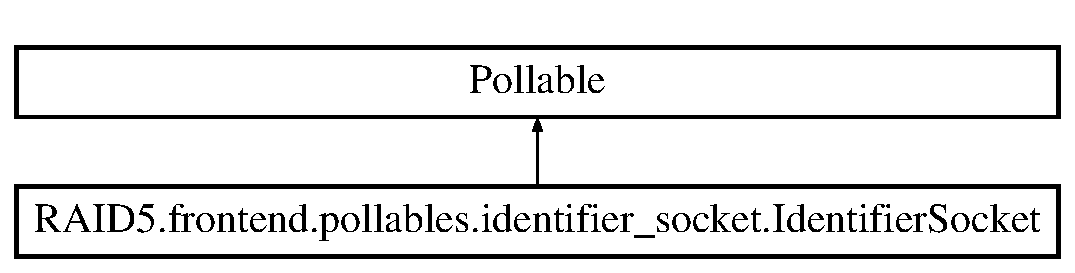
\includegraphics[height=2.000000cm]{class_r_a_i_d5_1_1frontend_1_1pollables_1_1identifier__socket_1_1_identifier_socket}
\end{center}
\end{figure}
\subsection*{Public Member Functions}
\begin{DoxyCompactItemize}
\item 
\mbox{\Hypertarget{class_r_a_i_d5_1_1frontend_1_1pollables_1_1identifier__socket_1_1_identifier_socket_a8eed7b16cfd893dd42a59fce881521c1}\label{class_r_a_i_d5_1_1frontend_1_1pollables_1_1identifier__socket_1_1_identifier_socket_a8eed7b16cfd893dd42a59fce881521c1}} 
def {\bfseries \+\_\+\+\_\+init\+\_\+\+\_\+} (self, socket, application\+\_\+context)
\item 
\mbox{\Hypertarget{class_r_a_i_d5_1_1frontend_1_1pollables_1_1identifier__socket_1_1_identifier_socket_a9071217114abc04bc1ba2505145a67d5}\label{class_r_a_i_d5_1_1frontend_1_1pollables_1_1identifier__socket_1_1_identifier_socket_a9071217114abc04bc1ba2505145a67d5}} 
def {\bfseries on\+\_\+idle} (self)
\item 
\mbox{\Hypertarget{class_r_a_i_d5_1_1frontend_1_1pollables_1_1identifier__socket_1_1_identifier_socket_a77dbcb31324ea1ca253d1c07c651cadf}\label{class_r_a_i_d5_1_1frontend_1_1pollables_1_1identifier__socket_1_1_identifier_socket_a77dbcb31324ea1ca253d1c07c651cadf}} 
def {\bfseries on\+\_\+read} (self)
\item 
\mbox{\Hypertarget{class_r_a_i_d5_1_1frontend_1_1pollables_1_1identifier__socket_1_1_identifier_socket_aeea9156bc7e45c4a56a1ef0e5cd98e10}\label{class_r_a_i_d5_1_1frontend_1_1pollables_1_1identifier__socket_1_1_identifier_socket_aeea9156bc7e45c4a56a1ef0e5cd98e10}} 
def {\bfseries update\+\_\+disconnected} (self)
\item 
\mbox{\Hypertarget{class_r_a_i_d5_1_1frontend_1_1pollables_1_1identifier__socket_1_1_identifier_socket_a5d97dea82d8a9302629998263808a241}\label{class_r_a_i_d5_1_1frontend_1_1pollables_1_1identifier__socket_1_1_identifier_socket_a5d97dea82d8a9302629998263808a241}} 
def {\bfseries update\+\_\+disk} (self, buf, address)
\item 
\mbox{\Hypertarget{class_r_a_i_d5_1_1frontend_1_1pollables_1_1identifier__socket_1_1_identifier_socket_a8c7a19e1c7fc4442bb7575cbbc67c92c}\label{class_r_a_i_d5_1_1frontend_1_1pollables_1_1identifier__socket_1_1_identifier_socket_a8c7a19e1c7fc4442bb7575cbbc67c92c}} 
def {\bfseries get\+\_\+events} (self)
\item 
\mbox{\Hypertarget{class_r_a_i_d5_1_1frontend_1_1pollables_1_1identifier__socket_1_1_identifier_socket_a25f496471418bc518d0d7d3d08849e6b}\label{class_r_a_i_d5_1_1frontend_1_1pollables_1_1identifier__socket_1_1_identifier_socket_a25f496471418bc518d0d7d3d08849e6b}} 
def {\bfseries is\+\_\+terminating} (self)
\item 
\mbox{\Hypertarget{class_r_a_i_d5_1_1frontend_1_1pollables_1_1identifier__socket_1_1_identifier_socket_aa5e4712638f9077c2c52df02de94d0aa}\label{class_r_a_i_d5_1_1frontend_1_1pollables_1_1identifier__socket_1_1_identifier_socket_aa5e4712638f9077c2c52df02de94d0aa}} 
def {\bfseries application\+\_\+context} (self)
\item 
\mbox{\Hypertarget{class_r_a_i_d5_1_1frontend_1_1pollables_1_1identifier__socket_1_1_identifier_socket_af3ce27c5fa65a4736846b310e647a6a6}\label{class_r_a_i_d5_1_1frontend_1_1pollables_1_1identifier__socket_1_1_identifier_socket_af3ce27c5fa65a4736846b310e647a6a6}} 
def {\bfseries application\+\_\+context} (self, a)
\item 
\mbox{\Hypertarget{class_r_a_i_d5_1_1frontend_1_1pollables_1_1identifier__socket_1_1_identifier_socket_a21158438292f7cb4c46f26cd30fd67d7}\label{class_r_a_i_d5_1_1frontend_1_1pollables_1_1identifier__socket_1_1_identifier_socket_a21158438292f7cb4c46f26cd30fd67d7}} 
def {\bfseries recvd\+\_\+data} (self)
\item 
\mbox{\Hypertarget{class_r_a_i_d5_1_1frontend_1_1pollables_1_1identifier__socket_1_1_identifier_socket_ab933f54d1265e4568a3e180102c2878c}\label{class_r_a_i_d5_1_1frontend_1_1pollables_1_1identifier__socket_1_1_identifier_socket_ab933f54d1265e4568a3e180102c2878c}} 
def {\bfseries recvd\+\_\+data} (self, r)
\item 
\mbox{\Hypertarget{class_r_a_i_d5_1_1frontend_1_1pollables_1_1identifier__socket_1_1_identifier_socket_add53f6e8348637d787da96b2a26f8b53}\label{class_r_a_i_d5_1_1frontend_1_1pollables_1_1identifier__socket_1_1_identifier_socket_add53f6e8348637d787da96b2a26f8b53}} 
def {\bfseries data\+\_\+to\+\_\+send} (self)
\item 
\mbox{\Hypertarget{class_r_a_i_d5_1_1frontend_1_1pollables_1_1identifier__socket_1_1_identifier_socket_a1648ebfa92b98c1288353eb69ba71a9d}\label{class_r_a_i_d5_1_1frontend_1_1pollables_1_1identifier__socket_1_1_identifier_socket_a1648ebfa92b98c1288353eb69ba71a9d}} 
def {\bfseries data\+\_\+to\+\_\+send} (self, d)
\item 
\mbox{\Hypertarget{class_r_a_i_d5_1_1frontend_1_1pollables_1_1identifier__socket_1_1_identifier_socket_a28fcb8da1ac305f70d3ea30fd0b23a81}\label{class_r_a_i_d5_1_1frontend_1_1pollables_1_1identifier__socket_1_1_identifier_socket_a28fcb8da1ac305f70d3ea30fd0b23a81}} 
def {\bfseries socket} (self)
\item 
\mbox{\Hypertarget{class_r_a_i_d5_1_1frontend_1_1pollables_1_1identifier__socket_1_1_identifier_socket_aaa61e5ec6e75f46f0c3eb4c7d8d736e8}\label{class_r_a_i_d5_1_1frontend_1_1pollables_1_1identifier__socket_1_1_identifier_socket_aaa61e5ec6e75f46f0c3eb4c7d8d736e8}} 
def {\bfseries fd} (self)
\item 
\mbox{\Hypertarget{class_r_a_i_d5_1_1frontend_1_1pollables_1_1identifier__socket_1_1_identifier_socket_ad090eb9bdfc48459afc2106aadb9ae49}\label{class_r_a_i_d5_1_1frontend_1_1pollables_1_1identifier__socket_1_1_identifier_socket_ad090eb9bdfc48459afc2106aadb9ae49}} 
def {\bfseries on\+\_\+error} (self, e)
\item 
\mbox{\Hypertarget{class_r_a_i_d5_1_1frontend_1_1pollables_1_1identifier__socket_1_1_identifier_socket_a5d1417912bb7777d5651711aafc2ca42}\label{class_r_a_i_d5_1_1frontend_1_1pollables_1_1identifier__socket_1_1_identifier_socket_a5d1417912bb7777d5651711aafc2ca42}} 
def {\bfseries on\+\_\+close} (self)
\item 
\mbox{\Hypertarget{class_r_a_i_d5_1_1frontend_1_1pollables_1_1identifier__socket_1_1_identifier_socket_a52af183b3f5f502c533d858bbc2a2822}\label{class_r_a_i_d5_1_1frontend_1_1pollables_1_1identifier__socket_1_1_identifier_socket_a52af183b3f5f502c533d858bbc2a2822}} 
def {\bfseries \+\_\+\+\_\+repr\+\_\+\+\_\+} (self)
\end{DoxyCompactItemize}


The documentation for this class was generated from the following file\+:\begin{DoxyCompactItemize}
\item 
C\+:/cygwin64/tmp/\+R\+A\+I\+D5/frontend/pollables/identifier\+\_\+socket.\+py\end{DoxyCompactItemize}

\hypertarget{class_r_a_i_d5_1_1frontend_1_1services_1_1init__service_1_1_init_service}{}\section{R\+A\+I\+D5.\+frontend.\+services.\+init\+\_\+service.\+Init\+Service Class Reference}
\label{class_r_a_i_d5_1_1frontend_1_1services_1_1init__service_1_1_init_service}\index{R\+A\+I\+D5.\+frontend.\+services.\+init\+\_\+service.\+Init\+Service@{R\+A\+I\+D5.\+frontend.\+services.\+init\+\_\+service.\+Init\+Service}}
Inheritance diagram for R\+A\+I\+D5.\+frontend.\+services.\+init\+\_\+service.\+Init\+Service\+:\begin{figure}[H]
\begin{center}
\leavevmode
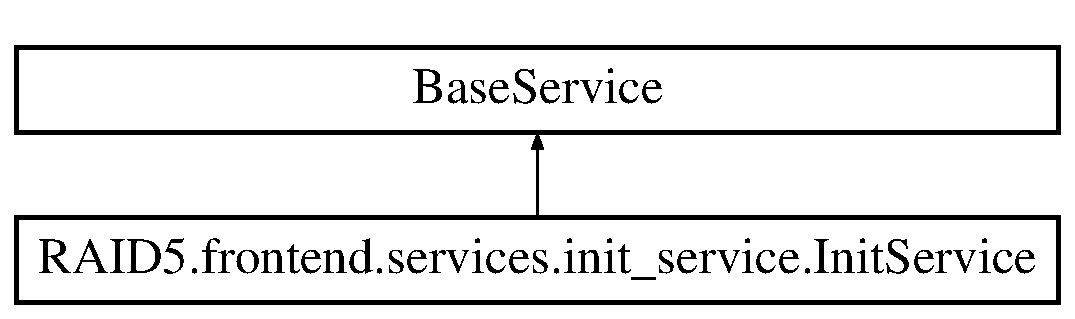
\includegraphics[height=2.000000cm]{class_r_a_i_d5_1_1frontend_1_1services_1_1init__service_1_1_init_service}
\end{center}
\end{figure}
\subsection*{Public Member Functions}
\begin{DoxyCompactItemize}
\item 
\mbox{\Hypertarget{class_r_a_i_d5_1_1frontend_1_1services_1_1init__service_1_1_init_service_a33d8573dfe235c77bcf7ce93bf9c85c6}\label{class_r_a_i_d5_1_1frontend_1_1services_1_1init__service_1_1_init_service_a33d8573dfe235c77bcf7ce93bf9c85c6}} 
def {\bfseries \+\_\+\+\_\+init\+\_\+\+\_\+} (self, entry, pollables, args)
\item 
\mbox{\Hypertarget{class_r_a_i_d5_1_1frontend_1_1services_1_1init__service_1_1_init_service_a9604d3a5936ea1bc504b71aff26823cb}\label{class_r_a_i_d5_1_1frontend_1_1services_1_1init__service_1_1_init_service_a9604d3a5936ea1bc504b71aff26823cb}} 
def {\bfseries before\+\_\+setup} (self, entry)
\item 
\mbox{\Hypertarget{class_r_a_i_d5_1_1frontend_1_1services_1_1init__service_1_1_init_service_a274d9154fb404ab95fb96f77a72da380}\label{class_r_a_i_d5_1_1frontend_1_1services_1_1init__service_1_1_init_service_a274d9154fb404ab95fb96f77a72da380}} 
def {\bfseries before\+\_\+login} (self, entry)
\item 
\mbox{\Hypertarget{class_r_a_i_d5_1_1frontend_1_1services_1_1init__service_1_1_init_service_aaddde01c20620171830854e09ac3fbfb}\label{class_r_a_i_d5_1_1frontend_1_1services_1_1init__service_1_1_init_service_aaddde01c20620171830854e09ac3fbfb}} 
def {\bfseries after\+\_\+login} (self, entry)
\item 
\mbox{\Hypertarget{class_r_a_i_d5_1_1frontend_1_1services_1_1init__service_1_1_init_service_ab06b5f4be3cb54d024307b2b4138fb80}\label{class_r_a_i_d5_1_1frontend_1_1services_1_1init__service_1_1_init_service_ab06b5f4be3cb54d024307b2b4138fb80}} 
def {\bfseries before\+\_\+existing\+\_\+mount} (self, entry)
\item 
\mbox{\Hypertarget{class_r_a_i_d5_1_1frontend_1_1services_1_1init__service_1_1_init_service_a3a51c09810c26b02947996376d247a68}\label{class_r_a_i_d5_1_1frontend_1_1services_1_1init__service_1_1_init_service_a3a51c09810c26b02947996376d247a68}} 
def {\bfseries after\+\_\+existing\+\_\+mount} (self, entry)
\item 
\mbox{\Hypertarget{class_r_a_i_d5_1_1frontend_1_1services_1_1init__service_1_1_init_service_a3fb0875724d736053698a0a10979309a}\label{class_r_a_i_d5_1_1frontend_1_1services_1_1init__service_1_1_init_service_a3fb0875724d736053698a0a10979309a}} 
def {\bfseries before\+\_\+scratch\+\_\+mount} (self, entry)
\item 
\mbox{\Hypertarget{class_r_a_i_d5_1_1frontend_1_1services_1_1init__service_1_1_init_service_a96b766af28b7658e58bd475acdf2e2d5}\label{class_r_a_i_d5_1_1frontend_1_1services_1_1init__service_1_1_init_service_a96b766af28b7658e58bd475acdf2e2d5}} 
def {\bfseries after\+\_\+scratch\+\_\+mount} (self, entry)
\item 
\mbox{\Hypertarget{class_r_a_i_d5_1_1frontend_1_1services_1_1init__service_1_1_init_service_a4c0071d394b7d0f510986e3198679807}\label{class_r_a_i_d5_1_1frontend_1_1services_1_1init__service_1_1_init_service_a4c0071d394b7d0f510986e3198679807}} 
def {\bfseries before\+\_\+response\+\_\+status} (self, entry)
\item 
\mbox{\Hypertarget{class_r_a_i_d5_1_1frontend_1_1services_1_1init__service_1_1_init_service_ab5b4ad94cdfd4b56e087f6f969ca9757}\label{class_r_a_i_d5_1_1frontend_1_1services_1_1init__service_1_1_init_service_ab5b4ad94cdfd4b56e087f6f969ca9757}} 
def {\bfseries before\+\_\+response\+\_\+headers} (self, entry)
\item 
\mbox{\Hypertarget{class_r_a_i_d5_1_1frontend_1_1services_1_1init__service_1_1_init_service_a4cfe73d9cd1eed1afdf84adaaf646814}\label{class_r_a_i_d5_1_1frontend_1_1services_1_1init__service_1_1_init_service_a4cfe73d9cd1eed1afdf84adaaf646814}} 
def {\bfseries before\+\_\+response\+\_\+content} (self, entry)
\item 
\mbox{\Hypertarget{class_r_a_i_d5_1_1frontend_1_1services_1_1init__service_1_1_init_service_ad058cb9a61cc91b0229f9227573e1476}\label{class_r_a_i_d5_1_1frontend_1_1services_1_1init__service_1_1_init_service_ad058cb9a61cc91b0229f9227573e1476}} 
def {\bfseries on\+\_\+finish} (self, entry)
\item 
\mbox{\Hypertarget{class_r_a_i_d5_1_1frontend_1_1services_1_1init__service_1_1_init_service_a0f3d065d12811e2d6ac2be5f98c912bb}\label{class_r_a_i_d5_1_1frontend_1_1services_1_1init__service_1_1_init_service_a0f3d065d12811e2d6ac2be5f98c912bb}} 
def {\bfseries create\+\_\+disk\+\_\+info\+\_\+content} (self, boundary, disk\+\_\+uuid, disks\+\_\+uuids)
\end{DoxyCompactItemize}
\subsection*{Static Public Member Functions}
\begin{DoxyCompactItemize}
\item 
\mbox{\Hypertarget{class_r_a_i_d5_1_1frontend_1_1services_1_1init__service_1_1_init_service_a0fb4dbcbec5c90e29da4a88e157e6457}\label{class_r_a_i_d5_1_1frontend_1_1services_1_1init__service_1_1_init_service_a0fb4dbcbec5c90e29da4a88e157e6457}} 
def {\bfseries get\+\_\+name} ()
\end{DoxyCompactItemize}
\subsection*{Static Public Attributes}
\begin{DoxyCompactItemize}
\item 
list {\bfseries S\+T\+A\+T\+ES}
\end{DoxyCompactItemize}


\subsection{Member Data Documentation}
\mbox{\Hypertarget{class_r_a_i_d5_1_1frontend_1_1services_1_1init__service_1_1_init_service_aeede04bcc77840ea29cbfa27f24c24cd}\label{class_r_a_i_d5_1_1frontend_1_1services_1_1init__service_1_1_init_service_aeede04bcc77840ea29cbfa27f24c24cd}} 
\index{R\+A\+I\+D5\+::frontend\+::services\+::init\+\_\+service\+::\+Init\+Service@{R\+A\+I\+D5\+::frontend\+::services\+::init\+\_\+service\+::\+Init\+Service}!S\+T\+A\+T\+ES@{S\+T\+A\+T\+ES}}
\index{S\+T\+A\+T\+ES@{S\+T\+A\+T\+ES}!R\+A\+I\+D5\+::frontend\+::services\+::init\+\_\+service\+::\+Init\+Service@{R\+A\+I\+D5\+::frontend\+::services\+::init\+\_\+service\+::\+Init\+Service}}
\subsubsection{\texorpdfstring{S\+T\+A\+T\+ES}{STATES}}
{\footnotesize\ttfamily list R\+A\+I\+D5.\+frontend.\+services.\+init\+\_\+service.\+Init\+Service.\+S\+T\+A\+T\+ES\hspace{0.3cm}{\ttfamily [static]}}

{\bfseries Initial value\+:}
\begin{DoxyCode}
=  [
        \hyperlink{classstate_1_1_state}{state.State}(
            SETUP\_STATE,
            [LOGIN\_STATE],
            before\_func=before\_setup
        ),
        \hyperlink{classstate_1_1_state}{state.State}(
            LOGIN\_STATE,
            [EXISTING\_MOUNT\_STATE, SCRATCH\_MOUNT\_STATE],  \textcolor{comment}{# order matters}
            before\_login,
            after\_login,
        ),
        \hyperlink{classstate_1_1_state}{state.State}(
            EXISTING\_MOUNT\_STATE,
            [FINAL\_STATE],
            before\_existing\_mount,
            after\_existing\_mount
        ),
        \hyperlink{classstate_1_1_state}{state.State}(
            SCRATCH\_MOUNT\_STATE,
            [FINAL\_STATE],
            before\_scratch\_mount,
            after\_scratch\_mount
        ),
        \hyperlink{classstate_1_1_state}{state.State}(
            FINAL\_STATE,
            [FINAL\_STATE]
        )
    ]
\end{DoxyCode}


The documentation for this class was generated from the following file\+:\begin{DoxyCompactItemize}
\item 
C\+:/cygwin64/tmp/\+R\+A\+I\+D5/frontend/services/init\+\_\+service.\+py\end{DoxyCompactItemize}

\hypertarget{class_r_a_i_d5_1_1common_1_1utilities_1_1util_1_1_invalid_arguments}{}\section{R\+A\+I\+D5.\+common.\+utilities.\+util.\+Invalid\+Arguments Class Reference}
\label{class_r_a_i_d5_1_1common_1_1utilities_1_1util_1_1_invalid_arguments}\index{R\+A\+I\+D5.\+common.\+utilities.\+util.\+Invalid\+Arguments@{R\+A\+I\+D5.\+common.\+utilities.\+util.\+Invalid\+Arguments}}
Inheritance diagram for R\+A\+I\+D5.\+common.\+utilities.\+util.\+Invalid\+Arguments\+:\begin{figure}[H]
\begin{center}
\leavevmode
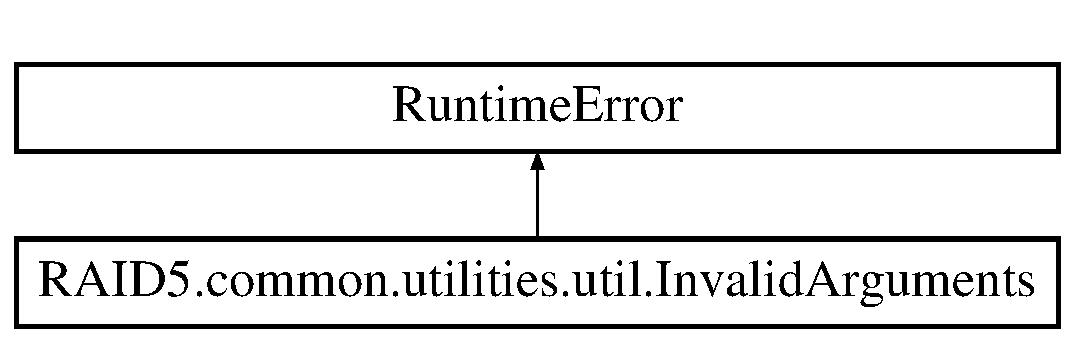
\includegraphics[height=2.000000cm]{class_r_a_i_d5_1_1common_1_1utilities_1_1util_1_1_invalid_arguments}
\end{center}
\end{figure}
\subsection*{Public Member Functions}
\begin{DoxyCompactItemize}
\item 
\mbox{\Hypertarget{class_r_a_i_d5_1_1common_1_1utilities_1_1util_1_1_invalid_arguments_a3df9ef60674910823a5c428ac26078f2}\label{class_r_a_i_d5_1_1common_1_1utilities_1_1util_1_1_invalid_arguments_a3df9ef60674910823a5c428ac26078f2}} 
def {\bfseries \+\_\+\+\_\+init\+\_\+\+\_\+} (self, desc=\char`\"{}Bad Arguments\char`\"{})
\end{DoxyCompactItemize}


The documentation for this class was generated from the following file\+:\begin{DoxyCompactItemize}
\item 
C\+:/cygwin64/tmp/\+R\+A\+I\+D5/common/utilities/util.\+py\end{DoxyCompactItemize}

\hypertarget{class_r_a_i_d5_1_1common_1_1pollables_1_1listener__socket_1_1_listener_socket}{}\section{R\+A\+I\+D5.\+common.\+pollables.\+listener\+\_\+socket.\+Listener\+Socket Class Reference}
\label{class_r_a_i_d5_1_1common_1_1pollables_1_1listener__socket_1_1_listener_socket}\index{R\+A\+I\+D5.\+common.\+pollables.\+listener\+\_\+socket.\+Listener\+Socket@{R\+A\+I\+D5.\+common.\+pollables.\+listener\+\_\+socket.\+Listener\+Socket}}
Inheritance diagram for R\+A\+I\+D5.\+common.\+pollables.\+listener\+\_\+socket.\+Listener\+Socket\+:\begin{figure}[H]
\begin{center}
\leavevmode
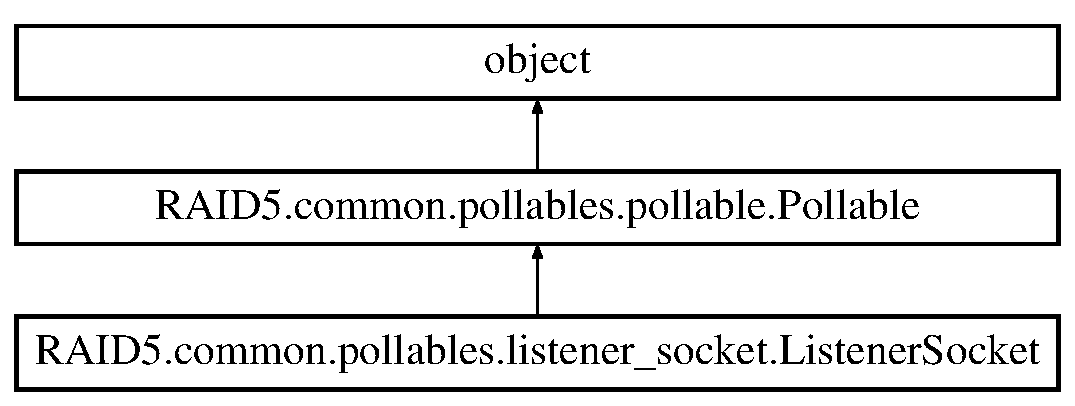
\includegraphics[height=3.000000cm]{class_r_a_i_d5_1_1common_1_1pollables_1_1listener__socket_1_1_listener_socket}
\end{center}
\end{figure}
\subsection*{Public Member Functions}
\begin{DoxyCompactItemize}
\item 
\mbox{\Hypertarget{class_r_a_i_d5_1_1common_1_1pollables_1_1listener__socket_1_1_listener_socket_a55fe4d345de76fd5509b5746a52a954b}\label{class_r_a_i_d5_1_1common_1_1pollables_1_1listener__socket_1_1_listener_socket_a55fe4d345de76fd5509b5746a52a954b}} 
def {\bfseries \+\_\+\+\_\+init\+\_\+\+\_\+} (self, socket, state, application\+\_\+context, pollables)
\item 
\mbox{\Hypertarget{class_r_a_i_d5_1_1common_1_1pollables_1_1listener__socket_1_1_listener_socket_aa19b6a3bab08b82014288aa40cf84943}\label{class_r_a_i_d5_1_1common_1_1pollables_1_1listener__socket_1_1_listener_socket_aa19b6a3bab08b82014288aa40cf84943}} 
def {\bfseries fd} (self)
\item 
\mbox{\Hypertarget{class_r_a_i_d5_1_1common_1_1pollables_1_1listener__socket_1_1_listener_socket_a91fbef7409f7c28249ed2503ac20b153}\label{class_r_a_i_d5_1_1common_1_1pollables_1_1listener__socket_1_1_listener_socket_a91fbef7409f7c28249ed2503ac20b153}} 
def {\bfseries socket} (self)
\item 
\mbox{\Hypertarget{class_r_a_i_d5_1_1common_1_1pollables_1_1listener__socket_1_1_listener_socket_a40fabe6db948b82c528cecb20263fe50}\label{class_r_a_i_d5_1_1common_1_1pollables_1_1listener__socket_1_1_listener_socket_a40fabe6db948b82c528cecb20263fe50}} 
def {\bfseries state} (self)
\item 
\mbox{\Hypertarget{class_r_a_i_d5_1_1common_1_1pollables_1_1listener__socket_1_1_listener_socket_ac79ad353902aa15d8bfe172953a32a6a}\label{class_r_a_i_d5_1_1common_1_1pollables_1_1listener__socket_1_1_listener_socket_ac79ad353902aa15d8bfe172953a32a6a}} 
def {\bfseries data\+\_\+to\+\_\+send} (self)
\item 
\mbox{\Hypertarget{class_r_a_i_d5_1_1common_1_1pollables_1_1listener__socket_1_1_listener_socket_a7de911cef40229fee54f77429ac86bf6}\label{class_r_a_i_d5_1_1common_1_1pollables_1_1listener__socket_1_1_listener_socket_a7de911cef40229fee54f77429ac86bf6}} 
def {\bfseries state} (self, s)
\item 
\mbox{\Hypertarget{class_r_a_i_d5_1_1common_1_1pollables_1_1listener__socket_1_1_listener_socket_aded4f5854bb030a50d43c33593666d1e}\label{class_r_a_i_d5_1_1common_1_1pollables_1_1listener__socket_1_1_listener_socket_aded4f5854bb030a50d43c33593666d1e}} 
def {\bfseries listen\+\_\+state} (self)
\item 
\mbox{\Hypertarget{class_r_a_i_d5_1_1common_1_1pollables_1_1listener__socket_1_1_listener_socket_ad9c1dbf5b99286520a01bd05ad3cd9c5}\label{class_r_a_i_d5_1_1common_1_1pollables_1_1listener__socket_1_1_listener_socket_ad9c1dbf5b99286520a01bd05ad3cd9c5}} 
def {\bfseries is\+\_\+terminating} (self)
\item 
\mbox{\Hypertarget{class_r_a_i_d5_1_1common_1_1pollables_1_1listener__socket_1_1_listener_socket_a24eb86c653e9bdfc1a6f74811d4e0e7e}\label{class_r_a_i_d5_1_1common_1_1pollables_1_1listener__socket_1_1_listener_socket_a24eb86c653e9bdfc1a6f74811d4e0e7e}} 
def {\bfseries on\+\_\+close} (self)
\item 
\mbox{\Hypertarget{class_r_a_i_d5_1_1common_1_1pollables_1_1listener__socket_1_1_listener_socket_ab4869f609510dbfc3e62c0cf3b3a94c9}\label{class_r_a_i_d5_1_1common_1_1pollables_1_1listener__socket_1_1_listener_socket_ab4869f609510dbfc3e62c0cf3b3a94c9}} 
def {\bfseries on\+\_\+read} (self)
\item 
\mbox{\Hypertarget{class_r_a_i_d5_1_1common_1_1pollables_1_1listener__socket_1_1_listener_socket_a1bc77108370b2ea303c39dcbb1cd21e7}\label{class_r_a_i_d5_1_1common_1_1pollables_1_1listener__socket_1_1_listener_socket_a1bc77108370b2ea303c39dcbb1cd21e7}} 
def {\bfseries on\+\_\+error} (self)
\item 
\mbox{\Hypertarget{class_r_a_i_d5_1_1common_1_1pollables_1_1listener__socket_1_1_listener_socket_a3c652be3e1852e323ee884e3e1a2a15b}\label{class_r_a_i_d5_1_1common_1_1pollables_1_1listener__socket_1_1_listener_socket_a3c652be3e1852e323ee884e3e1a2a15b}} 
def {\bfseries get\+\_\+events} (self)
\item 
\mbox{\Hypertarget{class_r_a_i_d5_1_1common_1_1pollables_1_1listener__socket_1_1_listener_socket_ae71c1fb4cc88198a858300b4eccdc70b}\label{class_r_a_i_d5_1_1common_1_1pollables_1_1listener__socket_1_1_listener_socket_ae71c1fb4cc88198a858300b4eccdc70b}} 
def {\bfseries \+\_\+\+\_\+repr\+\_\+\+\_\+} (self)
\end{DoxyCompactItemize}
\subsection*{Static Public Attributes}
\begin{DoxyCompactItemize}
\item 
dictionary {\bfseries states}
\end{DoxyCompactItemize}


\subsection{Member Data Documentation}
\mbox{\Hypertarget{class_r_a_i_d5_1_1common_1_1pollables_1_1listener__socket_1_1_listener_socket_aef6af91bec6de61b5d52a30efdf9acb0}\label{class_r_a_i_d5_1_1common_1_1pollables_1_1listener__socket_1_1_listener_socket_aef6af91bec6de61b5d52a30efdf9acb0}} 
\index{R\+A\+I\+D5\+::common\+::pollables\+::listener\+\_\+socket\+::\+Listener\+Socket@{R\+A\+I\+D5\+::common\+::pollables\+::listener\+\_\+socket\+::\+Listener\+Socket}!states@{states}}
\index{states@{states}!R\+A\+I\+D5\+::common\+::pollables\+::listener\+\_\+socket\+::\+Listener\+Socket@{R\+A\+I\+D5\+::common\+::pollables\+::listener\+\_\+socket\+::\+Listener\+Socket}}
\subsubsection{\texorpdfstring{states}{states}}
{\footnotesize\ttfamily dictionary R\+A\+I\+D5.\+common.\+pollables.\+listener\+\_\+socket.\+Listener\+Socket.\+states\hspace{0.3cm}{\ttfamily [static]}}

{\bfseries Initial value\+:}
\begin{DoxyCode}
=  \{
        constants.LISTEN\_STATE: \{
            \textcolor{stringliteral}{"function"}: listen\_state,
            \textcolor{stringliteral}{"next"}: constants.CLOSING\_STATE
        \},
        constants.CLOSING\_STATE: \{
            \textcolor{stringliteral}{"function"}: on\_close,
            \textcolor{stringliteral}{"next"}: constants.CLOSING\_STATE,
        \}
    \}
\end{DoxyCode}


The documentation for this class was generated from the following file\+:\begin{DoxyCompactItemize}
\item 
C\+:/cygwin64/tmp/\+R\+A\+I\+D5/common/pollables/listener\+\_\+socket.\+py\end{DoxyCompactItemize}

\hypertarget{class_r_a_i_d5_1_1block__device_1_1services_1_1login__service_1_1_login_service}{}\section{R\+A\+I\+D5.\+block\+\_\+device.\+services.\+login\+\_\+service.\+Login\+Service Class Reference}
\label{class_r_a_i_d5_1_1block__device_1_1services_1_1login__service_1_1_login_service}\index{R\+A\+I\+D5.\+block\+\_\+device.\+services.\+login\+\_\+service.\+Login\+Service@{R\+A\+I\+D5.\+block\+\_\+device.\+services.\+login\+\_\+service.\+Login\+Service}}


A Block Device Service that allows the Frontend to supply it with a long\+\_\+password for later communication.  


Inheritance diagram for R\+A\+I\+D5.\+block\+\_\+device.\+services.\+login\+\_\+service.\+Login\+Service\+:\begin{figure}[H]
\begin{center}
\leavevmode
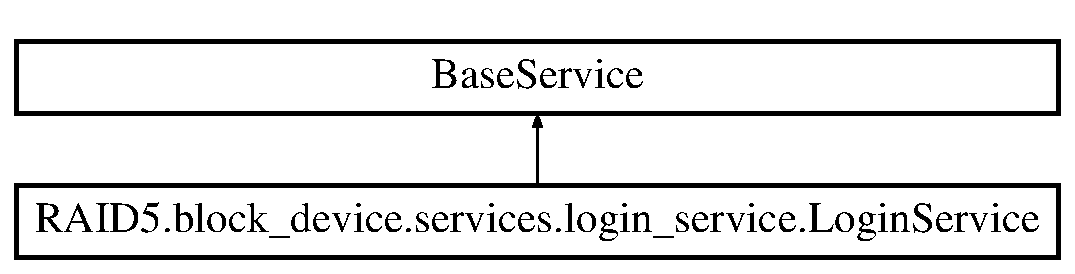
\includegraphics[height=2.000000cm]{class_r_a_i_d5_1_1block__device_1_1services_1_1login__service_1_1_login_service}
\end{center}
\end{figure}
\subsection*{Public Member Functions}
\begin{DoxyCompactItemize}
\item 
def \hyperlink{class_r_a_i_d5_1_1block__device_1_1services_1_1login__service_1_1_login_service_a3e9d974a2333ef0cb54874b65842ca53}{\+\_\+\+\_\+init\+\_\+\+\_\+} (self, entry, pollables, args)
\begin{DoxyCompactList}\small\item\em Constructor for \hyperlink{class_r_a_i_d5_1_1block__device_1_1services_1_1login__service_1_1_login_service}{Login\+Service}. \end{DoxyCompactList}\item 
def \hyperlink{class_r_a_i_d5_1_1block__device_1_1services_1_1login__service_1_1_login_service_a0dbcb210b5b1bbd67a0321b86c21824f}{handle\+\_\+content} (self, entry, content)
\begin{DoxyCompactList}\small\item\em Handle the content that entry socket has recieved extract the password and volume\+\_\+\+U\+U\+ID from frontend request. \end{DoxyCompactList}\item 
def \hyperlink{class_r_a_i_d5_1_1block__device_1_1services_1_1login__service_1_1_login_service_ad6279990022af1400907394ad4fb2fb4}{before\+\_\+response\+\_\+status} (self, entry)
\begin{DoxyCompactList}\small\item\em What the service does before sending a response status function reads the block requested from the disk file. \end{DoxyCompactList}\end{DoxyCompactItemize}
\subsection*{Static Public Member Functions}
\begin{DoxyCompactItemize}
\item 
def \hyperlink{class_r_a_i_d5_1_1block__device_1_1services_1_1login__service_1_1_login_service_a8501e68a944ed20a107108801926b1be}{get\+\_\+name} ()
\begin{DoxyCompactList}\small\item\em Name of the service needed for Frontend purposes, creating clients required by \hyperlink{class_r_a_i_d5_1_1common_1_1services_1_1base__service_1_1_base_service}{common.\+services.\+base\+\_\+service.\+Base\+Service}. \end{DoxyCompactList}\end{DoxyCompactItemize}


\subsection{Detailed Description}
A Block Device Service that allows the Frontend to supply it with a long\+\_\+password for later communication. 

\subsection{Constructor \& Destructor Documentation}
\mbox{\Hypertarget{class_r_a_i_d5_1_1block__device_1_1services_1_1login__service_1_1_login_service_a3e9d974a2333ef0cb54874b65842ca53}\label{class_r_a_i_d5_1_1block__device_1_1services_1_1login__service_1_1_login_service_a3e9d974a2333ef0cb54874b65842ca53}} 
\index{R\+A\+I\+D5\+::block\+\_\+device\+::services\+::login\+\_\+service\+::\+Login\+Service@{R\+A\+I\+D5\+::block\+\_\+device\+::services\+::login\+\_\+service\+::\+Login\+Service}!\+\_\+\+\_\+init\+\_\+\+\_\+@{\+\_\+\+\_\+init\+\_\+\+\_\+}}
\index{\+\_\+\+\_\+init\+\_\+\+\_\+@{\+\_\+\+\_\+init\+\_\+\+\_\+}!R\+A\+I\+D5\+::block\+\_\+device\+::services\+::login\+\_\+service\+::\+Login\+Service@{R\+A\+I\+D5\+::block\+\_\+device\+::services\+::login\+\_\+service\+::\+Login\+Service}}
\subsubsection{\texorpdfstring{\+\_\+\+\_\+init\+\_\+\+\_\+()}{\_\_init\_\_()}}
{\footnotesize\ttfamily def R\+A\+I\+D5.\+block\+\_\+device.\+services.\+login\+\_\+service.\+Login\+Service.\+\_\+\+\_\+init\+\_\+\+\_\+ (\begin{DoxyParamCaption}\item[{}]{self,  }\item[{}]{entry,  }\item[{}]{pollables,  }\item[{}]{args }\end{DoxyParamCaption})}



Constructor for \hyperlink{class_r_a_i_d5_1_1block__device_1_1services_1_1login__service_1_1_login_service}{Login\+Service}. 


\begin{DoxyParams}{Parameters}
{\em entry} & (entry) the entry (probably common.\+pollables.\+service\+\_\+socket) using the service \\
\hline
{\em pollables} & (dict) All the pollables currently in the server \\
\hline
{\em args} & (dict) Arguments for this service \\
\hline
\end{DoxyParams}


\subsection{Member Function Documentation}
\mbox{\Hypertarget{class_r_a_i_d5_1_1block__device_1_1services_1_1login__service_1_1_login_service_ad6279990022af1400907394ad4fb2fb4}\label{class_r_a_i_d5_1_1block__device_1_1services_1_1login__service_1_1_login_service_ad6279990022af1400907394ad4fb2fb4}} 
\index{R\+A\+I\+D5\+::block\+\_\+device\+::services\+::login\+\_\+service\+::\+Login\+Service@{R\+A\+I\+D5\+::block\+\_\+device\+::services\+::login\+\_\+service\+::\+Login\+Service}!before\+\_\+response\+\_\+status@{before\+\_\+response\+\_\+status}}
\index{before\+\_\+response\+\_\+status@{before\+\_\+response\+\_\+status}!R\+A\+I\+D5\+::block\+\_\+device\+::services\+::login\+\_\+service\+::\+Login\+Service@{R\+A\+I\+D5\+::block\+\_\+device\+::services\+::login\+\_\+service\+::\+Login\+Service}}
\subsubsection{\texorpdfstring{before\+\_\+response\+\_\+status()}{before\_response\_status()}}
{\footnotesize\ttfamily def R\+A\+I\+D5.\+block\+\_\+device.\+services.\+login\+\_\+service.\+Login\+Service.\+before\+\_\+response\+\_\+status (\begin{DoxyParamCaption}\item[{}]{self,  }\item[{}]{entry }\end{DoxyParamCaption})}



What the service does before sending a response status function reads the block requested from the disk file. 


\begin{DoxyParams}{Parameters}
{\em entry} & (pollable) the entry that the service is assigned to \\
\hline
\end{DoxyParams}
\begin{DoxyReturn}{Returns}
(bool) if finished and ready to move on 
\end{DoxyReturn}
\mbox{\Hypertarget{class_r_a_i_d5_1_1block__device_1_1services_1_1login__service_1_1_login_service_a8501e68a944ed20a107108801926b1be}\label{class_r_a_i_d5_1_1block__device_1_1services_1_1login__service_1_1_login_service_a8501e68a944ed20a107108801926b1be}} 
\index{R\+A\+I\+D5\+::block\+\_\+device\+::services\+::login\+\_\+service\+::\+Login\+Service@{R\+A\+I\+D5\+::block\+\_\+device\+::services\+::login\+\_\+service\+::\+Login\+Service}!get\+\_\+name@{get\+\_\+name}}
\index{get\+\_\+name@{get\+\_\+name}!R\+A\+I\+D5\+::block\+\_\+device\+::services\+::login\+\_\+service\+::\+Login\+Service@{R\+A\+I\+D5\+::block\+\_\+device\+::services\+::login\+\_\+service\+::\+Login\+Service}}
\subsubsection{\texorpdfstring{get\+\_\+name()}{get\_name()}}
{\footnotesize\ttfamily def R\+A\+I\+D5.\+block\+\_\+device.\+services.\+login\+\_\+service.\+Login\+Service.\+get\+\_\+name (\begin{DoxyParamCaption}{ }\end{DoxyParamCaption})\hspace{0.3cm}{\ttfamily [static]}}



Name of the service needed for Frontend purposes, creating clients required by \hyperlink{class_r_a_i_d5_1_1common_1_1services_1_1base__service_1_1_base_service}{common.\+services.\+base\+\_\+service.\+Base\+Service}. 

\begin{DoxyReturn}{Returns}
(str) service name 
\end{DoxyReturn}
\mbox{\Hypertarget{class_r_a_i_d5_1_1block__device_1_1services_1_1login__service_1_1_login_service_a0dbcb210b5b1bbd67a0321b86c21824f}\label{class_r_a_i_d5_1_1block__device_1_1services_1_1login__service_1_1_login_service_a0dbcb210b5b1bbd67a0321b86c21824f}} 
\index{R\+A\+I\+D5\+::block\+\_\+device\+::services\+::login\+\_\+service\+::\+Login\+Service@{R\+A\+I\+D5\+::block\+\_\+device\+::services\+::login\+\_\+service\+::\+Login\+Service}!handle\+\_\+content@{handle\+\_\+content}}
\index{handle\+\_\+content@{handle\+\_\+content}!R\+A\+I\+D5\+::block\+\_\+device\+::services\+::login\+\_\+service\+::\+Login\+Service@{R\+A\+I\+D5\+::block\+\_\+device\+::services\+::login\+\_\+service\+::\+Login\+Service}}
\subsubsection{\texorpdfstring{handle\+\_\+content()}{handle\_content()}}
{\footnotesize\ttfamily def R\+A\+I\+D5.\+block\+\_\+device.\+services.\+login\+\_\+service.\+Login\+Service.\+handle\+\_\+content (\begin{DoxyParamCaption}\item[{}]{self,  }\item[{}]{entry,  }\item[{}]{content }\end{DoxyParamCaption})}



Handle the content that entry socket has recieved extract the password and volume\+\_\+\+U\+U\+ID from frontend request. 


\begin{DoxyParams}{Parameters}
{\em entry} & (pollable) the entry that the service is assigned to \\
\hline
{\em content} & (str) content recieved from the frontend \\
\hline
\end{DoxyParams}


The documentation for this class was generated from the following file\+:\begin{DoxyCompactItemize}
\item 
C\+:/cygwin64/tmp/\+R\+A\+I\+D5/block\+\_\+device/services/login\+\_\+service.\+py\end{DoxyCompactItemize}

\hypertarget{class_r_a_i_d5_1_1frontend_1_1services_1_1management__service_1_1_management_service}{}\section{R\+A\+I\+D5.\+frontend.\+services.\+management\+\_\+service.\+Management\+Service Class Reference}
\label{class_r_a_i_d5_1_1frontend_1_1services_1_1management__service_1_1_management_service}\index{R\+A\+I\+D5.\+frontend.\+services.\+management\+\_\+service.\+Management\+Service@{R\+A\+I\+D5.\+frontend.\+services.\+management\+\_\+service.\+Management\+Service}}
Inheritance diagram for R\+A\+I\+D5.\+frontend.\+services.\+management\+\_\+service.\+Management\+Service\+:\begin{figure}[H]
\begin{center}
\leavevmode
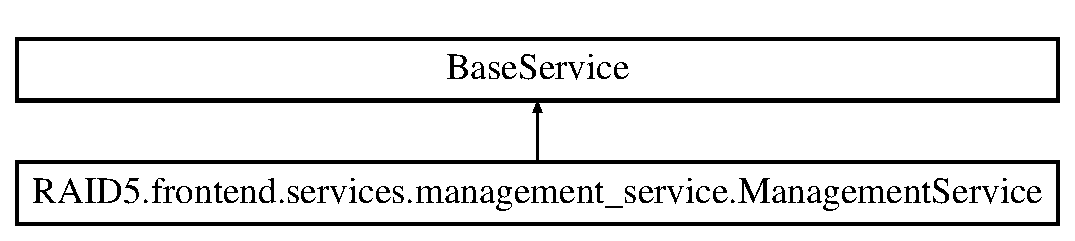
\includegraphics[height=2.000000cm]{class_r_a_i_d5_1_1frontend_1_1services_1_1management__service_1_1_management_service}
\end{center}
\end{figure}
\subsection*{Public Member Functions}
\begin{DoxyCompactItemize}
\item 
\mbox{\Hypertarget{class_r_a_i_d5_1_1frontend_1_1services_1_1management__service_1_1_management_service_a9f06b873fd105ad219ac8b67fa26a142}\label{class_r_a_i_d5_1_1frontend_1_1services_1_1management__service_1_1_management_service_a9f06b873fd105ad219ac8b67fa26a142}} 
def {\bfseries \+\_\+\+\_\+init\+\_\+\+\_\+} (self, entry, pollables, args)
\item 
\mbox{\Hypertarget{class_r_a_i_d5_1_1frontend_1_1services_1_1management__service_1_1_management_service_a434179507908785a212e155c7ce28301}\label{class_r_a_i_d5_1_1frontend_1_1services_1_1management__service_1_1_management_service_a434179507908785a212e155c7ce28301}} 
def {\bfseries before\+\_\+response\+\_\+headers} (self, entry)
\end{DoxyCompactItemize}
\subsection*{Static Public Member Functions}
\begin{DoxyCompactItemize}
\item 
\mbox{\Hypertarget{class_r_a_i_d5_1_1frontend_1_1services_1_1management__service_1_1_management_service_a31b7c8602e2dd72f68c0d2a596c936fd}\label{class_r_a_i_d5_1_1frontend_1_1services_1_1management__service_1_1_management_service_a31b7c8602e2dd72f68c0d2a596c936fd}} 
def {\bfseries get\+\_\+name} ()
\end{DoxyCompactItemize}


The documentation for this class was generated from the following file\+:\begin{DoxyCompactItemize}
\item 
C\+:/cygwin64/tmp/\+R\+A\+I\+D5/frontend/services/management\+\_\+service.\+py\end{DoxyCompactItemize}

\hypertarget{class_r_a_i_d5_1_1frontend_1_1services_1_1mul__service_1_1_mul_service}{}\section{R\+A\+I\+D5.\+frontend.\+services.\+mul\+\_\+service.\+Mul\+Service Class Reference}
\label{class_r_a_i_d5_1_1frontend_1_1services_1_1mul__service_1_1_mul_service}\index{R\+A\+I\+D5.\+frontend.\+services.\+mul\+\_\+service.\+Mul\+Service@{R\+A\+I\+D5.\+frontend.\+services.\+mul\+\_\+service.\+Mul\+Service}}
Inheritance diagram for R\+A\+I\+D5.\+frontend.\+services.\+mul\+\_\+service.\+Mul\+Service\+:\begin{figure}[H]
\begin{center}
\leavevmode
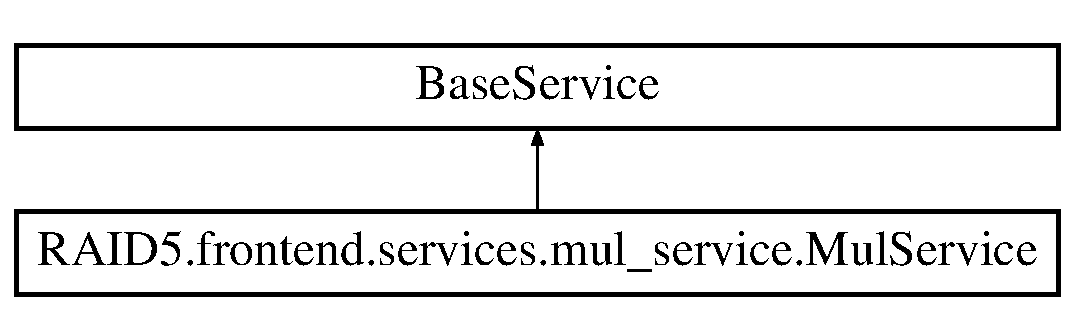
\includegraphics[height=2.000000cm]{class_r_a_i_d5_1_1frontend_1_1services_1_1mul__service_1_1_mul_service}
\end{center}
\end{figure}
\subsection*{Public Member Functions}
\begin{DoxyCompactItemize}
\item 
\mbox{\Hypertarget{class_r_a_i_d5_1_1frontend_1_1services_1_1mul__service_1_1_mul_service_a33fae624e124be5282402ad1d59314c4}\label{class_r_a_i_d5_1_1frontend_1_1services_1_1mul__service_1_1_mul_service_a33fae624e124be5282402ad1d59314c4}} 
def {\bfseries \+\_\+\+\_\+init\+\_\+\+\_\+} (self, entry, pollables, args)
\item 
\mbox{\Hypertarget{class_r_a_i_d5_1_1frontend_1_1services_1_1mul__service_1_1_mul_service_ab52fdcb7a31a197e56e4786366dec465}\label{class_r_a_i_d5_1_1frontend_1_1services_1_1mul__service_1_1_mul_service_ab52fdcb7a31a197e56e4786366dec465}} 
def {\bfseries before\+\_\+response\+\_\+status} (self, entry)
\end{DoxyCompactItemize}
\subsection*{Static Public Member Functions}
\begin{DoxyCompactItemize}
\item 
\mbox{\Hypertarget{class_r_a_i_d5_1_1frontend_1_1services_1_1mul__service_1_1_mul_service_af0746d143f29e41f6e872eb63fd3e0eb}\label{class_r_a_i_d5_1_1frontend_1_1services_1_1mul__service_1_1_mul_service_af0746d143f29e41f6e872eb63fd3e0eb}} 
def {\bfseries get\+\_\+name} ()
\end{DoxyCompactItemize}


The documentation for this class was generated from the following file\+:\begin{DoxyCompactItemize}
\item 
C\+:/cygwin64/tmp/\+R\+A\+I\+D5/frontend/services/mul\+\_\+service.\+py\end{DoxyCompactItemize}

\hypertarget{class_r_a_i_d5_1_1common_1_1pollables_1_1pollable_1_1_pollable}{}\section{R\+A\+I\+D5.\+common.\+pollables.\+pollable.\+Pollable Class Reference}
\label{class_r_a_i_d5_1_1common_1_1pollables_1_1pollable_1_1_pollable}\index{R\+A\+I\+D5.\+common.\+pollables.\+pollable.\+Pollable@{R\+A\+I\+D5.\+common.\+pollables.\+pollable.\+Pollable}}
Inheritance diagram for R\+A\+I\+D5.\+common.\+pollables.\+pollable.\+Pollable\+:\begin{figure}[H]
\begin{center}
\leavevmode
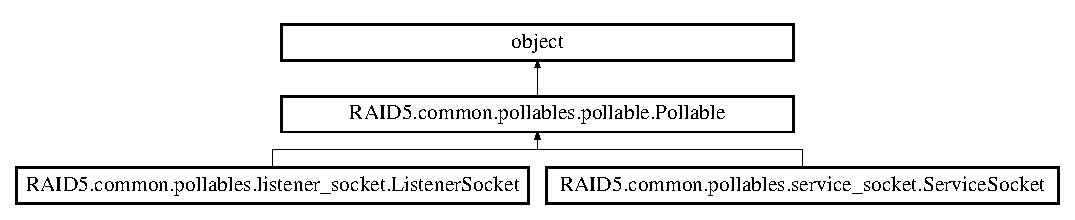
\includegraphics[height=2.507463cm]{class_r_a_i_d5_1_1common_1_1pollables_1_1pollable_1_1_pollable}
\end{center}
\end{figure}
\subsection*{Public Member Functions}
\begin{DoxyCompactItemize}
\item 
\mbox{\Hypertarget{class_r_a_i_d5_1_1common_1_1pollables_1_1pollable_1_1_pollable_af261ececf5f5e21d95611e7a1a9b01e3}\label{class_r_a_i_d5_1_1common_1_1pollables_1_1pollable_1_1_pollable_af261ececf5f5e21d95611e7a1a9b01e3}} 
def {\bfseries on\+\_\+idle} (self)
\item 
\mbox{\Hypertarget{class_r_a_i_d5_1_1common_1_1pollables_1_1pollable_1_1_pollable_a9a989d7ddd2aa7ffcaa349c0e9f47880}\label{class_r_a_i_d5_1_1common_1_1pollables_1_1pollable_1_1_pollable_a9a989d7ddd2aa7ffcaa349c0e9f47880}} 
def {\bfseries on\+\_\+read} (self)
\item 
\mbox{\Hypertarget{class_r_a_i_d5_1_1common_1_1pollables_1_1pollable_1_1_pollable_ac98ba12dcc8968d74b0b11bc083315de}\label{class_r_a_i_d5_1_1common_1_1pollables_1_1pollable_1_1_pollable_ac98ba12dcc8968d74b0b11bc083315de}} 
def {\bfseries on\+\_\+write} (self)
\item 
\mbox{\Hypertarget{class_r_a_i_d5_1_1common_1_1pollables_1_1pollable_1_1_pollable_ad31d3a7892af98c5e5e51e1bbb69b7b0}\label{class_r_a_i_d5_1_1common_1_1pollables_1_1pollable_1_1_pollable_ad31d3a7892af98c5e5e51e1bbb69b7b0}} 
def {\bfseries on\+\_\+error} (self)
\item 
\mbox{\Hypertarget{class_r_a_i_d5_1_1common_1_1pollables_1_1pollable_1_1_pollable_a14860df1cb88e4cfa7e5ce0a066e55c6}\label{class_r_a_i_d5_1_1common_1_1pollables_1_1pollable_1_1_pollable_a14860df1cb88e4cfa7e5ce0a066e55c6}} 
def {\bfseries get\+\_\+events} (self)
\item 
\mbox{\Hypertarget{class_r_a_i_d5_1_1common_1_1pollables_1_1pollable_1_1_pollable_aad042c9fbe6554403349310be32824c7}\label{class_r_a_i_d5_1_1common_1_1pollables_1_1pollable_1_1_pollable_aad042c9fbe6554403349310be32824c7}} 
def {\bfseries is\+\_\+terminating} (self)
\end{DoxyCompactItemize}


The documentation for this class was generated from the following file\+:\begin{DoxyCompactItemize}
\item 
C\+:/cygwin64/tmp/\+R\+A\+I\+D5/common/pollables/pollable.\+py\end{DoxyCompactItemize}

\hypertarget{class_r_a_i_d5_1_1common_1_1utilities_1_1poller_1_1_poller}{}\section{R\+A\+I\+D5.\+common.\+utilities.\+poller.\+Poller Class Reference}
\label{class_r_a_i_d5_1_1common_1_1utilities_1_1poller_1_1_poller}\index{R\+A\+I\+D5.\+common.\+utilities.\+poller.\+Poller@{R\+A\+I\+D5.\+common.\+utilities.\+poller.\+Poller}}
\subsection*{Public Member Functions}
\begin{DoxyCompactItemize}
\item 
\mbox{\Hypertarget{class_r_a_i_d5_1_1common_1_1utilities_1_1poller_1_1_poller_af5d855a67c680b7d8a11c508d9238746}\label{class_r_a_i_d5_1_1common_1_1utilities_1_1poller_1_1_poller_af5d855a67c680b7d8a11c508d9238746}} 
def {\bfseries \+\_\+\+\_\+init\+\_\+\+\_\+} (self)
\item 
\mbox{\Hypertarget{class_r_a_i_d5_1_1common_1_1utilities_1_1poller_1_1_poller_ab2f49582a72257205602f142d87a4b02}\label{class_r_a_i_d5_1_1common_1_1utilities_1_1poller_1_1_poller_ab2f49582a72257205602f142d87a4b02}} 
def {\bfseries register} (self, fd, event)
\item 
\mbox{\Hypertarget{class_r_a_i_d5_1_1common_1_1utilities_1_1poller_1_1_poller_af85695b10f249fe19709c4aa62a9ac03}\label{class_r_a_i_d5_1_1common_1_1utilities_1_1poller_1_1_poller_af85695b10f249fe19709c4aa62a9ac03}} 
def {\bfseries poll} (self, timeout)
\end{DoxyCompactItemize}


The documentation for this class was generated from the following file\+:\begin{DoxyCompactItemize}
\item 
C\+:/cygwin64/tmp/\+R\+A\+I\+D5/common/utilities/poller.\+py\end{DoxyCompactItemize}

\hypertarget{class_r_a_i_d5_1_1frontend_1_1services_1_1read__disk__service_1_1_read_from_disk_service}{}\section{R\+A\+I\+D5.\+frontend.\+services.\+read\+\_\+disk\+\_\+service.\+Read\+From\+Disk\+Service Class Reference}
\label{class_r_a_i_d5_1_1frontend_1_1services_1_1read__disk__service_1_1_read_from_disk_service}\index{R\+A\+I\+D5.\+frontend.\+services.\+read\+\_\+disk\+\_\+service.\+Read\+From\+Disk\+Service@{R\+A\+I\+D5.\+frontend.\+services.\+read\+\_\+disk\+\_\+service.\+Read\+From\+Disk\+Service}}
Inheritance diagram for R\+A\+I\+D5.\+frontend.\+services.\+read\+\_\+disk\+\_\+service.\+Read\+From\+Disk\+Service\+:\begin{figure}[H]
\begin{center}
\leavevmode
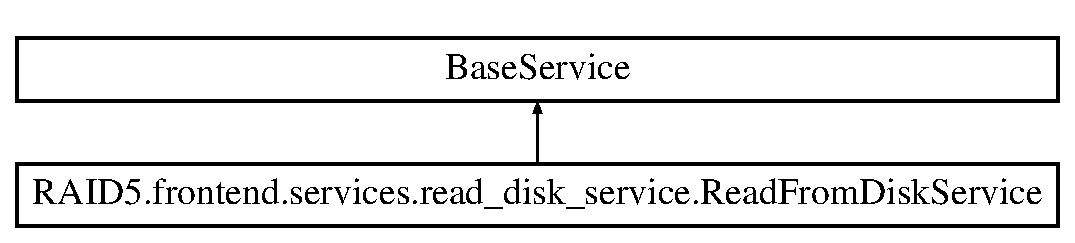
\includegraphics[height=2.000000cm]{class_r_a_i_d5_1_1frontend_1_1services_1_1read__disk__service_1_1_read_from_disk_service}
\end{center}
\end{figure}
\subsection*{Public Member Functions}
\begin{DoxyCompactItemize}
\item 
\mbox{\Hypertarget{class_r_a_i_d5_1_1frontend_1_1services_1_1read__disk__service_1_1_read_from_disk_service_af6e96ebf1fe3caa1b622f583e28ee1a6}\label{class_r_a_i_d5_1_1frontend_1_1services_1_1read__disk__service_1_1_read_from_disk_service_af6e96ebf1fe3caa1b622f583e28ee1a6}} 
def {\bfseries \+\_\+\+\_\+init\+\_\+\+\_\+} (self, entry, pollables, args)
\item 
\mbox{\Hypertarget{class_r_a_i_d5_1_1frontend_1_1services_1_1read__disk__service_1_1_read_from_disk_service_a483d0702aea39cc7c8e4a2cb6948c2b1}\label{class_r_a_i_d5_1_1frontend_1_1services_1_1read__disk__service_1_1_read_from_disk_service_a483d0702aea39cc7c8e4a2cb6948c2b1}} 
def {\bfseries before\+\_\+read} (self, entry)
\item 
\mbox{\Hypertarget{class_r_a_i_d5_1_1frontend_1_1services_1_1read__disk__service_1_1_read_from_disk_service_a80d58e9bda9f8c58f950a167a4c8e90b}\label{class_r_a_i_d5_1_1frontend_1_1services_1_1read__disk__service_1_1_read_from_disk_service_a80d58e9bda9f8c58f950a167a4c8e90b}} 
def {\bfseries after\+\_\+read} (self, entry)
\item 
\mbox{\Hypertarget{class_r_a_i_d5_1_1frontend_1_1services_1_1read__disk__service_1_1_read_from_disk_service_a9f770e79f079264842daa3ecdd2890ef}\label{class_r_a_i_d5_1_1frontend_1_1services_1_1read__disk__service_1_1_read_from_disk_service_a9f770e79f079264842daa3ecdd2890ef}} 
def {\bfseries update\+\_\+block} (self)
\item 
\mbox{\Hypertarget{class_r_a_i_d5_1_1frontend_1_1services_1_1read__disk__service_1_1_read_from_disk_service_a85b0aab4db9ba90e4b21cee925335489}\label{class_r_a_i_d5_1_1frontend_1_1services_1_1read__disk__service_1_1_read_from_disk_service_a85b0aab4db9ba90e4b21cee925335489}} 
def {\bfseries before\+\_\+response\+\_\+status} (self, entry)
\item 
\mbox{\Hypertarget{class_r_a_i_d5_1_1frontend_1_1services_1_1read__disk__service_1_1_read_from_disk_service_a10fc777a0d6da5fc7fd0309c23e06500}\label{class_r_a_i_d5_1_1frontend_1_1services_1_1read__disk__service_1_1_read_from_disk_service_a10fc777a0d6da5fc7fd0309c23e06500}} 
def {\bfseries before\+\_\+response\+\_\+content} (self, entry)
\item 
\mbox{\Hypertarget{class_r_a_i_d5_1_1frontend_1_1services_1_1read__disk__service_1_1_read_from_disk_service_ad3cba811a6cc1557ffd0960d2a155d39}\label{class_r_a_i_d5_1_1frontend_1_1services_1_1read__disk__service_1_1_read_from_disk_service_ad3cba811a6cc1557ffd0960d2a155d39}} 
def {\bfseries on\+\_\+finish} (self, entry)
\end{DoxyCompactItemize}
\subsection*{Static Public Member Functions}
\begin{DoxyCompactItemize}
\item 
\mbox{\Hypertarget{class_r_a_i_d5_1_1frontend_1_1services_1_1read__disk__service_1_1_read_from_disk_service_a0288014b9af6315bdeed89b702c4a6ca}\label{class_r_a_i_d5_1_1frontend_1_1services_1_1read__disk__service_1_1_read_from_disk_service_a0288014b9af6315bdeed89b702c4a6ca}} 
def {\bfseries get\+\_\+name} ()
\end{DoxyCompactItemize}
\subsection*{Static Public Attributes}
\begin{DoxyCompactItemize}
\item 
list {\bfseries S\+T\+A\+T\+ES}
\end{DoxyCompactItemize}


\subsection{Member Data Documentation}
\mbox{\Hypertarget{class_r_a_i_d5_1_1frontend_1_1services_1_1read__disk__service_1_1_read_from_disk_service_a0d38c5ec13adcb1a772d9025fe564eac}\label{class_r_a_i_d5_1_1frontend_1_1services_1_1read__disk__service_1_1_read_from_disk_service_a0d38c5ec13adcb1a772d9025fe564eac}} 
\index{R\+A\+I\+D5\+::frontend\+::services\+::read\+\_\+disk\+\_\+service\+::\+Read\+From\+Disk\+Service@{R\+A\+I\+D5\+::frontend\+::services\+::read\+\_\+disk\+\_\+service\+::\+Read\+From\+Disk\+Service}!S\+T\+A\+T\+ES@{S\+T\+A\+T\+ES}}
\index{S\+T\+A\+T\+ES@{S\+T\+A\+T\+ES}!R\+A\+I\+D5\+::frontend\+::services\+::read\+\_\+disk\+\_\+service\+::\+Read\+From\+Disk\+Service@{R\+A\+I\+D5\+::frontend\+::services\+::read\+\_\+disk\+\_\+service\+::\+Read\+From\+Disk\+Service}}
\subsubsection{\texorpdfstring{S\+T\+A\+T\+ES}{STATES}}
{\footnotesize\ttfamily list R\+A\+I\+D5.\+frontend.\+services.\+read\+\_\+disk\+\_\+service.\+Read\+From\+Disk\+Service.\+S\+T\+A\+T\+ES\hspace{0.3cm}{\ttfamily [static]}}

{\bfseries Initial value\+:}
\begin{DoxyCode}
=  [
        \hyperlink{classstate_1_1_state}{state.State}(
            READ\_STATE,
            [READ\_STATE, FINAL\_STATE],
            before\_read,
            after\_read
        ),
        \hyperlink{classstate_1_1_state}{state.State}(
            FINAL\_STATE,
            [FINAL\_STATE]
        )
    ]
\end{DoxyCode}


The documentation for this class was generated from the following file\+:\begin{DoxyCompactItemize}
\item 
C\+:/cygwin64/tmp/\+R\+A\+I\+D5/frontend/services/read\+\_\+disk\+\_\+service.\+py\end{DoxyCompactItemize}

\hypertarget{class_r_a_i_d5_1_1common_1_1utilities_1_1poller_1_1_select}{}\section{R\+A\+I\+D5.\+common.\+utilities.\+poller.\+Select Class Reference}
\label{class_r_a_i_d5_1_1common_1_1utilities_1_1poller_1_1_select}\index{R\+A\+I\+D5.\+common.\+utilities.\+poller.\+Select@{R\+A\+I\+D5.\+common.\+utilities.\+poller.\+Select}}
\subsection*{Public Member Functions}
\begin{DoxyCompactItemize}
\item 
\mbox{\Hypertarget{class_r_a_i_d5_1_1common_1_1utilities_1_1poller_1_1_select_a4e90bc039ac43cb00783237f88617b9c}\label{class_r_a_i_d5_1_1common_1_1utilities_1_1poller_1_1_select_a4e90bc039ac43cb00783237f88617b9c}} 
def {\bfseries \+\_\+\+\_\+init\+\_\+\+\_\+} (self)
\item 
\mbox{\Hypertarget{class_r_a_i_d5_1_1common_1_1utilities_1_1poller_1_1_select_a7415a0da66a75827102528640ad3abce}\label{class_r_a_i_d5_1_1common_1_1utilities_1_1poller_1_1_select_a7415a0da66a75827102528640ad3abce}} 
def {\bfseries register} (self, fd, event)
\item 
\mbox{\Hypertarget{class_r_a_i_d5_1_1common_1_1utilities_1_1poller_1_1_select_a9c6235184e1937bdf9a0f384058888c0}\label{class_r_a_i_d5_1_1common_1_1utilities_1_1poller_1_1_select_a9c6235184e1937bdf9a0f384058888c0}} 
def {\bfseries poll} (self, timeout)
\end{DoxyCompactItemize}


The documentation for this class was generated from the following file\+:\begin{DoxyCompactItemize}
\item 
C\+:/cygwin64/tmp/\+R\+A\+I\+D5/common/utilities/poller.\+py\end{DoxyCompactItemize}

\hypertarget{class_r_a_i_d5_1_1common_1_1pollables_1_1service__socket_1_1_service_socket}{}\section{R\+A\+I\+D5.\+common.\+pollables.\+service\+\_\+socket.\+Service\+Socket Class Reference}
\label{class_r_a_i_d5_1_1common_1_1pollables_1_1service__socket_1_1_service_socket}\index{R\+A\+I\+D5.\+common.\+pollables.\+service\+\_\+socket.\+Service\+Socket@{R\+A\+I\+D5.\+common.\+pollables.\+service\+\_\+socket.\+Service\+Socket}}
Inheritance diagram for R\+A\+I\+D5.\+common.\+pollables.\+service\+\_\+socket.\+Service\+Socket\+:\begin{figure}[H]
\begin{center}
\leavevmode
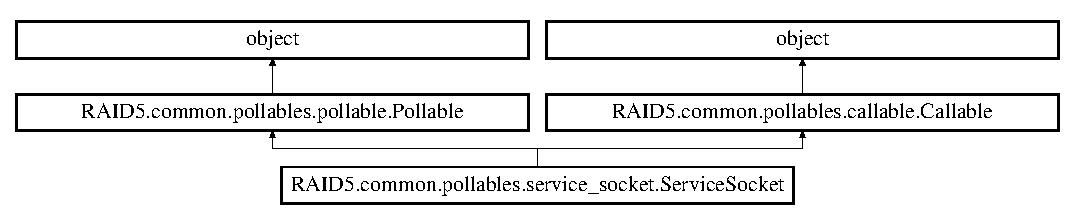
\includegraphics[height=2.507463cm]{class_r_a_i_d5_1_1common_1_1pollables_1_1service__socket_1_1_service_socket}
\end{center}
\end{figure}
\subsection*{Public Member Functions}
\begin{DoxyCompactItemize}
\item 
\mbox{\Hypertarget{class_r_a_i_d5_1_1common_1_1pollables_1_1service__socket_1_1_service_socket_aa37f60ce85767535ae437ae926057405}\label{class_r_a_i_d5_1_1common_1_1pollables_1_1service__socket_1_1_service_socket_aa37f60ce85767535ae437ae926057405}} 
def {\bfseries \+\_\+\+\_\+init\+\_\+\+\_\+} (self, socket, state, application\+\_\+context, pollables)
\item 
\mbox{\Hypertarget{class_r_a_i_d5_1_1common_1_1pollables_1_1service__socket_1_1_service_socket_aa00d55ea0cf280379664b94051f168b9}\label{class_r_a_i_d5_1_1common_1_1pollables_1_1service__socket_1_1_service_socket_aa00d55ea0cf280379664b94051f168b9}} 
def {\bfseries state} (self)
\item 
\mbox{\Hypertarget{class_r_a_i_d5_1_1common_1_1pollables_1_1service__socket_1_1_service_socket_a5717b88a33ee738784d3cd8ebf415c53}\label{class_r_a_i_d5_1_1common_1_1pollables_1_1service__socket_1_1_service_socket_a5717b88a33ee738784d3cd8ebf415c53}} 
def {\bfseries state} (self, s)
\item 
\mbox{\Hypertarget{class_r_a_i_d5_1_1common_1_1pollables_1_1service__socket_1_1_service_socket_ab6a20ec6f16cb5bf3b109440b5c58cdd}\label{class_r_a_i_d5_1_1common_1_1pollables_1_1service__socket_1_1_service_socket_ab6a20ec6f16cb5bf3b109440b5c58cdd}} 
def {\bfseries service} (self)
\item 
\mbox{\Hypertarget{class_r_a_i_d5_1_1common_1_1pollables_1_1service__socket_1_1_service_socket_a1064eeacf2bef53a2122f35bad730930}\label{class_r_a_i_d5_1_1common_1_1pollables_1_1service__socket_1_1_service_socket_a1064eeacf2bef53a2122f35bad730930}} 
def {\bfseries service} (self, s)
\item 
\mbox{\Hypertarget{class_r_a_i_d5_1_1common_1_1pollables_1_1service__socket_1_1_service_socket_ae71e1607a20dee704a27ee80baff27e3}\label{class_r_a_i_d5_1_1common_1_1pollables_1_1service__socket_1_1_service_socket_ae71e1607a20dee704a27ee80baff27e3}} 
def {\bfseries request\+\_\+context} (self)
\item 
\mbox{\Hypertarget{class_r_a_i_d5_1_1common_1_1pollables_1_1service__socket_1_1_service_socket_a8fcbf86d200b90f985fb4b6913ad5278}\label{class_r_a_i_d5_1_1common_1_1pollables_1_1service__socket_1_1_service_socket_a8fcbf86d200b90f985fb4b6913ad5278}} 
def {\bfseries request\+\_\+context} (self, r)
\item 
\mbox{\Hypertarget{class_r_a_i_d5_1_1common_1_1pollables_1_1service__socket_1_1_service_socket_ac0af9ad2453d8fd5c1f2ac583dfa6a12}\label{class_r_a_i_d5_1_1common_1_1pollables_1_1service__socket_1_1_service_socket_ac0af9ad2453d8fd5c1f2ac583dfa6a12}} 
def {\bfseries application\+\_\+context} (self)
\item 
\mbox{\Hypertarget{class_r_a_i_d5_1_1common_1_1pollables_1_1service__socket_1_1_service_socket_a3793da962466f99f434476db35a78e73}\label{class_r_a_i_d5_1_1common_1_1pollables_1_1service__socket_1_1_service_socket_a3793da962466f99f434476db35a78e73}} 
def {\bfseries application\+\_\+context} (self, a)
\item 
\mbox{\Hypertarget{class_r_a_i_d5_1_1common_1_1pollables_1_1service__socket_1_1_service_socket_ad1d9e95ba2844a70707be8de088c97c2}\label{class_r_a_i_d5_1_1common_1_1pollables_1_1service__socket_1_1_service_socket_ad1d9e95ba2844a70707be8de088c97c2}} 
def {\bfseries recvd\+\_\+data} (self)
\item 
\mbox{\Hypertarget{class_r_a_i_d5_1_1common_1_1pollables_1_1service__socket_1_1_service_socket_a6be56df95a6ceab7d6b4961ca23885a7}\label{class_r_a_i_d5_1_1common_1_1pollables_1_1service__socket_1_1_service_socket_a6be56df95a6ceab7d6b4961ca23885a7}} 
def {\bfseries recvd\+\_\+data} (self, r)
\item 
\mbox{\Hypertarget{class_r_a_i_d5_1_1common_1_1pollables_1_1service__socket_1_1_service_socket_ad5b737e15f07ea4c93c94df38eb8fb3c}\label{class_r_a_i_d5_1_1common_1_1pollables_1_1service__socket_1_1_service_socket_ad5b737e15f07ea4c93c94df38eb8fb3c}} 
def {\bfseries data\+\_\+to\+\_\+send} (self)
\item 
\mbox{\Hypertarget{class_r_a_i_d5_1_1common_1_1pollables_1_1service__socket_1_1_service_socket_a0c05c887886e7aca7520d12b2cc01069}\label{class_r_a_i_d5_1_1common_1_1pollables_1_1service__socket_1_1_service_socket_a0c05c887886e7aca7520d12b2cc01069}} 
def {\bfseries data\+\_\+to\+\_\+send} (self, d)
\item 
\mbox{\Hypertarget{class_r_a_i_d5_1_1common_1_1pollables_1_1service__socket_1_1_service_socket_a7234abc36e8da022ca0f667e53211bce}\label{class_r_a_i_d5_1_1common_1_1pollables_1_1service__socket_1_1_service_socket_a7234abc36e8da022ca0f667e53211bce}} 
def {\bfseries socket} (self)
\item 
\mbox{\Hypertarget{class_r_a_i_d5_1_1common_1_1pollables_1_1service__socket_1_1_service_socket_aeafcc304b19dbc7b6a2b590f7511d3f3}\label{class_r_a_i_d5_1_1common_1_1pollables_1_1service__socket_1_1_service_socket_aeafcc304b19dbc7b6a2b590f7511d3f3}} 
def {\bfseries fd} (self)
\item 
\mbox{\Hypertarget{class_r_a_i_d5_1_1common_1_1pollables_1_1service__socket_1_1_service_socket_a62b5bfbf85b6f83a50e9c19067d21061}\label{class_r_a_i_d5_1_1common_1_1pollables_1_1service__socket_1_1_service_socket_a62b5bfbf85b6f83a50e9c19067d21061}} 
def {\bfseries on\+\_\+error} (self, e)
\item 
\mbox{\Hypertarget{class_r_a_i_d5_1_1common_1_1pollables_1_1service__socket_1_1_service_socket_a18e9999ffe364ef69528a4eb5c1ff3e1}\label{class_r_a_i_d5_1_1common_1_1pollables_1_1service__socket_1_1_service_socket_a18e9999ffe364ef69528a4eb5c1ff3e1}} 
def {\bfseries on\+\_\+close} (self)
\item 
\mbox{\Hypertarget{class_r_a_i_d5_1_1common_1_1pollables_1_1service__socket_1_1_service_socket_a10732eed4fd6dbcb41cc3ede3aad3574}\label{class_r_a_i_d5_1_1common_1_1pollables_1_1service__socket_1_1_service_socket_a10732eed4fd6dbcb41cc3ede3aad3574}} 
def {\bfseries is\+\_\+terminating} (self)
\item 
\mbox{\Hypertarget{class_r_a_i_d5_1_1common_1_1pollables_1_1service__socket_1_1_service_socket_a36efc03fa6b7616bb5f587fc8303cab1}\label{class_r_a_i_d5_1_1common_1_1pollables_1_1service__socket_1_1_service_socket_a36efc03fa6b7616bb5f587fc8303cab1}} 
def {\bfseries on\+\_\+read} (self)
\item 
\mbox{\Hypertarget{class_r_a_i_d5_1_1common_1_1pollables_1_1service__socket_1_1_service_socket_ab3095ac9d51ca7f20d4ea406a1d0a600}\label{class_r_a_i_d5_1_1common_1_1pollables_1_1service__socket_1_1_service_socket_ab3095ac9d51ca7f20d4ea406a1d0a600}} 
def {\bfseries on\+\_\+finish} (self)
\item 
\mbox{\Hypertarget{class_r_a_i_d5_1_1common_1_1pollables_1_1service__socket_1_1_service_socket_a297e3f0bb748323ca4bc0ddb2dfeca64}\label{class_r_a_i_d5_1_1common_1_1pollables_1_1service__socket_1_1_service_socket_a297e3f0bb748323ca4bc0ddb2dfeca64}} 
def {\bfseries on\+\_\+write} (self)
\item 
\mbox{\Hypertarget{class_r_a_i_d5_1_1common_1_1pollables_1_1service__socket_1_1_service_socket_a6805b8374b843f8ceed93690bb9b5107}\label{class_r_a_i_d5_1_1common_1_1pollables_1_1service__socket_1_1_service_socket_a6805b8374b843f8ceed93690bb9b5107}} 
def {\bfseries get\+\_\+events} (self)
\item 
\mbox{\Hypertarget{class_r_a_i_d5_1_1common_1_1pollables_1_1service__socket_1_1_service_socket_a8d066c9c871edd28aced9543a8bbe2ce}\label{class_r_a_i_d5_1_1common_1_1pollables_1_1service__socket_1_1_service_socket_a8d066c9c871edd28aced9543a8bbe2ce}} 
def {\bfseries \+\_\+\+\_\+repr\+\_\+\+\_\+} (self)
\item 
\mbox{\Hypertarget{class_r_a_i_d5_1_1common_1_1pollables_1_1service__socket_1_1_service_socket_a38666cc9497d03062debb9707fb728bf}\label{class_r_a_i_d5_1_1common_1_1pollables_1_1service__socket_1_1_service_socket_a38666cc9497d03062debb9707fb728bf}} 
def {\bfseries handle\+\_\+request} (self, request)
\end{DoxyCompactItemize}
\subsection*{Static Public Attributes}
\begin{DoxyCompactItemize}
\item 
dictionary {\bfseries states}
\end{DoxyCompactItemize}


\subsection{Member Data Documentation}
\mbox{\Hypertarget{class_r_a_i_d5_1_1common_1_1pollables_1_1service__socket_1_1_service_socket_ad0ecb236e7b9b06c14b220a70e50f600}\label{class_r_a_i_d5_1_1common_1_1pollables_1_1service__socket_1_1_service_socket_ad0ecb236e7b9b06c14b220a70e50f600}} 
\index{R\+A\+I\+D5\+::common\+::pollables\+::service\+\_\+socket\+::\+Service\+Socket@{R\+A\+I\+D5\+::common\+::pollables\+::service\+\_\+socket\+::\+Service\+Socket}!states@{states}}
\index{states@{states}!R\+A\+I\+D5\+::common\+::pollables\+::service\+\_\+socket\+::\+Service\+Socket@{R\+A\+I\+D5\+::common\+::pollables\+::service\+\_\+socket\+::\+Service\+Socket}}
\subsubsection{\texorpdfstring{states}{states}}
{\footnotesize\ttfamily dictionary R\+A\+I\+D5.\+common.\+pollables.\+service\+\_\+socket.\+Service\+Socket.\+states\hspace{0.3cm}{\ttfamily [static]}}

{\bfseries Initial value\+:}
\begin{DoxyCode}
=  \{
        constants.GET\_REQUEST\_STATE: \{
            \textcolor{stringliteral}{"function"}: http\_util.get\_request\_state,
            \textcolor{stringliteral}{"next"}: constants.GET\_HEADERS\_STATE
        \},
        constants.GET\_HEADERS\_STATE: \{
            \textcolor{stringliteral}{"function"}: http\_util.get\_headers\_state,
            \textcolor{stringliteral}{"next"}: constants.GET\_CONTENT\_STATE
        \},
        constants.GET\_CONTENT\_STATE: \{
            \textcolor{stringliteral}{"function"}: http\_util.get\_content\_state,
            \textcolor{stringliteral}{"next"}: constants.SEND\_STATUS\_STATE
        \},
        constants.SEND\_STATUS\_STATE: \{
            \textcolor{stringliteral}{"function"}: http\_util.send\_status\_state,
            \textcolor{stringliteral}{"next"}: constants.SEND\_HEADERS\_STATE,
        \},
        constants.SEND\_HEADERS\_STATE: \{
            \textcolor{stringliteral}{"function"}: http\_util.send\_headers\_state,
            \textcolor{stringliteral}{"next"}: constants.SEND\_CONTENT\_STATE,
        \},
        constants.SEND\_CONTENT\_STATE: \{
            \textcolor{stringliteral}{"function"}: http\_util.send\_content\_state,
            \textcolor{stringliteral}{"next"}: constants.CLOSING\_STATE,
        \},
        constants.CLOSING\_STATE: \{
            \textcolor{stringliteral}{"function"}: on\_error,  \textcolor{comment}{# should change to more appropriate name}
            \textcolor{stringliteral}{"next"}: constants.CLOSING\_STATE,
        \}
    \}
\end{DoxyCode}


The documentation for this class was generated from the following file\+:\begin{DoxyCompactItemize}
\item 
C\+:/cygwin64/tmp/\+R\+A\+I\+D5/common/pollables/service\+\_\+socket.\+py\end{DoxyCompactItemize}

\hypertarget{class_r_a_i_d5_1_1block__device_1_1services_1_1set__block__service_1_1_set_block_service}{}\section{R\+A\+I\+D5.\+block\+\_\+device.\+services.\+set\+\_\+block\+\_\+service.\+Set\+Block\+Service Class Reference}
\label{class_r_a_i_d5_1_1block__device_1_1services_1_1set__block__service_1_1_set_block_service}\index{R\+A\+I\+D5.\+block\+\_\+device.\+services.\+set\+\_\+block\+\_\+service.\+Set\+Block\+Service@{R\+A\+I\+D5.\+block\+\_\+device.\+services.\+set\+\_\+block\+\_\+service.\+Set\+Block\+Service}}


A Block Device Service that allows the Frontend Server to set a block.  


Inheritance diagram for R\+A\+I\+D5.\+block\+\_\+device.\+services.\+set\+\_\+block\+\_\+service.\+Set\+Block\+Service\+:\begin{figure}[H]
\begin{center}
\leavevmode
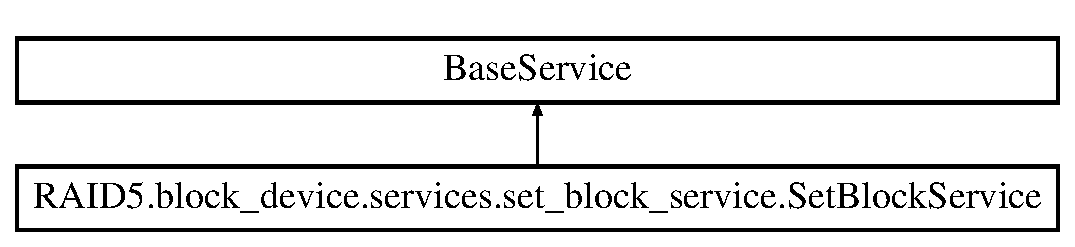
\includegraphics[height=2.000000cm]{class_r_a_i_d5_1_1block__device_1_1services_1_1set__block__service_1_1_set_block_service}
\end{center}
\end{figure}
\subsection*{Public Member Functions}
\begin{DoxyCompactItemize}
\item 
def \hyperlink{class_r_a_i_d5_1_1block__device_1_1services_1_1set__block__service_1_1_set_block_service_a591d47df0e924696ac23450906f5ddf2}{\+\_\+\+\_\+init\+\_\+\+\_\+} (self, entry, pollables, args)
\begin{DoxyCompactList}\small\item\em Constructor for Get\+Block\+Service. \end{DoxyCompactList}\item 
def \hyperlink{class_r_a_i_d5_1_1block__device_1_1services_1_1set__block__service_1_1_set_block_service_a00766fb59a3f4118444ab9265cb9e9d2}{before\+\_\+content} (self, entry)
\begin{DoxyCompactList}\small\item\em What the service does before recieving the content function prepares the file descriptor for writing in correct place. \end{DoxyCompactList}\item 
def \hyperlink{class_r_a_i_d5_1_1block__device_1_1services_1_1set__block__service_1_1_set_block_service_ac79d1b55a4e34943fa1e4f9514d9891d}{handle\+\_\+content} (self, entry, content)
\begin{DoxyCompactList}\small\item\em Handle the content that entry socket has recieved write to disk file with file desciptor. \end{DoxyCompactList}\item 
\mbox{\Hypertarget{class_r_a_i_d5_1_1block__device_1_1services_1_1set__block__service_1_1_set_block_service_af727ae5baf474b50749faaff9f6f7811}\label{class_r_a_i_d5_1_1block__device_1_1services_1_1set__block__service_1_1_set_block_service_af727ae5baf474b50749faaff9f6f7811}} 
def \hyperlink{class_r_a_i_d5_1_1block__device_1_1services_1_1set__block__service_1_1_set_block_service_af727ae5baf474b50749faaff9f6f7811}{before\+\_\+terminate} (self, entry)
\begin{DoxyCompactList}\small\item\em What the service needs to do before terminating closes the disk file descriptor. \end{DoxyCompactList}\end{DoxyCompactItemize}
\subsection*{Static Public Member Functions}
\begin{DoxyCompactItemize}
\item 
def \hyperlink{class_r_a_i_d5_1_1block__device_1_1services_1_1set__block__service_1_1_set_block_service_a8278d215309ac794164fa430a9727cc2}{get\+\_\+name} ()
\begin{DoxyCompactList}\small\item\em Name of the service needed for Frontend purposes, creating clients required by \hyperlink{class_r_a_i_d5_1_1common_1_1services_1_1base__service_1_1_base_service}{common.\+services.\+base\+\_\+service.\+Base\+Service}. \end{DoxyCompactList}\end{DoxyCompactItemize}


\subsection{Detailed Description}
A Block Device Service that allows the Frontend Server to set a block. 

\subsection{Constructor \& Destructor Documentation}
\mbox{\Hypertarget{class_r_a_i_d5_1_1block__device_1_1services_1_1set__block__service_1_1_set_block_service_a591d47df0e924696ac23450906f5ddf2}\label{class_r_a_i_d5_1_1block__device_1_1services_1_1set__block__service_1_1_set_block_service_a591d47df0e924696ac23450906f5ddf2}} 
\index{R\+A\+I\+D5\+::block\+\_\+device\+::services\+::set\+\_\+block\+\_\+service\+::\+Set\+Block\+Service@{R\+A\+I\+D5\+::block\+\_\+device\+::services\+::set\+\_\+block\+\_\+service\+::\+Set\+Block\+Service}!\+\_\+\+\_\+init\+\_\+\+\_\+@{\+\_\+\+\_\+init\+\_\+\+\_\+}}
\index{\+\_\+\+\_\+init\+\_\+\+\_\+@{\+\_\+\+\_\+init\+\_\+\+\_\+}!R\+A\+I\+D5\+::block\+\_\+device\+::services\+::set\+\_\+block\+\_\+service\+::\+Set\+Block\+Service@{R\+A\+I\+D5\+::block\+\_\+device\+::services\+::set\+\_\+block\+\_\+service\+::\+Set\+Block\+Service}}
\subsubsection{\texorpdfstring{\+\_\+\+\_\+init\+\_\+\+\_\+()}{\_\_init\_\_()}}
{\footnotesize\ttfamily def R\+A\+I\+D5.\+block\+\_\+device.\+services.\+set\+\_\+block\+\_\+service.\+Set\+Block\+Service.\+\_\+\+\_\+init\+\_\+\+\_\+ (\begin{DoxyParamCaption}\item[{}]{self,  }\item[{}]{entry,  }\item[{}]{pollables,  }\item[{}]{args }\end{DoxyParamCaption})}



Constructor for Get\+Block\+Service. 


\begin{DoxyParams}{Parameters}
{\em entry} & (pollable) the entry (probably common.\+pollables.\+service\+\_\+socket) using the service \\
\hline
{\em pollables} & (dict) All the pollables currently in the server \\
\hline
{\em args} & (dict) Arguments for this service \\
\hline
\end{DoxyParams}


\subsection{Member Function Documentation}
\mbox{\Hypertarget{class_r_a_i_d5_1_1block__device_1_1services_1_1set__block__service_1_1_set_block_service_a00766fb59a3f4118444ab9265cb9e9d2}\label{class_r_a_i_d5_1_1block__device_1_1services_1_1set__block__service_1_1_set_block_service_a00766fb59a3f4118444ab9265cb9e9d2}} 
\index{R\+A\+I\+D5\+::block\+\_\+device\+::services\+::set\+\_\+block\+\_\+service\+::\+Set\+Block\+Service@{R\+A\+I\+D5\+::block\+\_\+device\+::services\+::set\+\_\+block\+\_\+service\+::\+Set\+Block\+Service}!before\+\_\+content@{before\+\_\+content}}
\index{before\+\_\+content@{before\+\_\+content}!R\+A\+I\+D5\+::block\+\_\+device\+::services\+::set\+\_\+block\+\_\+service\+::\+Set\+Block\+Service@{R\+A\+I\+D5\+::block\+\_\+device\+::services\+::set\+\_\+block\+\_\+service\+::\+Set\+Block\+Service}}
\subsubsection{\texorpdfstring{before\+\_\+content()}{before\_content()}}
{\footnotesize\ttfamily def R\+A\+I\+D5.\+block\+\_\+device.\+services.\+set\+\_\+block\+\_\+service.\+Set\+Block\+Service.\+before\+\_\+content (\begin{DoxyParamCaption}\item[{}]{self,  }\item[{}]{entry }\end{DoxyParamCaption})}



What the service does before recieving the content function prepares the file descriptor for writing in correct place. 


\begin{DoxyParams}{Parameters}
{\em entry} & (pollable) the entry that the service is assigned to \\
\hline
\end{DoxyParams}
\begin{DoxyReturn}{Returns}
(bool) if finished and ready to move on 
\end{DoxyReturn}
\mbox{\Hypertarget{class_r_a_i_d5_1_1block__device_1_1services_1_1set__block__service_1_1_set_block_service_a8278d215309ac794164fa430a9727cc2}\label{class_r_a_i_d5_1_1block__device_1_1services_1_1set__block__service_1_1_set_block_service_a8278d215309ac794164fa430a9727cc2}} 
\index{R\+A\+I\+D5\+::block\+\_\+device\+::services\+::set\+\_\+block\+\_\+service\+::\+Set\+Block\+Service@{R\+A\+I\+D5\+::block\+\_\+device\+::services\+::set\+\_\+block\+\_\+service\+::\+Set\+Block\+Service}!get\+\_\+name@{get\+\_\+name}}
\index{get\+\_\+name@{get\+\_\+name}!R\+A\+I\+D5\+::block\+\_\+device\+::services\+::set\+\_\+block\+\_\+service\+::\+Set\+Block\+Service@{R\+A\+I\+D5\+::block\+\_\+device\+::services\+::set\+\_\+block\+\_\+service\+::\+Set\+Block\+Service}}
\subsubsection{\texorpdfstring{get\+\_\+name()}{get\_name()}}
{\footnotesize\ttfamily def R\+A\+I\+D5.\+block\+\_\+device.\+services.\+set\+\_\+block\+\_\+service.\+Set\+Block\+Service.\+get\+\_\+name (\begin{DoxyParamCaption}{ }\end{DoxyParamCaption})\hspace{0.3cm}{\ttfamily [static]}}



Name of the service needed for Frontend purposes, creating clients required by \hyperlink{class_r_a_i_d5_1_1common_1_1services_1_1base__service_1_1_base_service}{common.\+services.\+base\+\_\+service.\+Base\+Service}. 

\begin{DoxyReturn}{Returns}
(str) service name 
\end{DoxyReturn}
\mbox{\Hypertarget{class_r_a_i_d5_1_1block__device_1_1services_1_1set__block__service_1_1_set_block_service_ac79d1b55a4e34943fa1e4f9514d9891d}\label{class_r_a_i_d5_1_1block__device_1_1services_1_1set__block__service_1_1_set_block_service_ac79d1b55a4e34943fa1e4f9514d9891d}} 
\index{R\+A\+I\+D5\+::block\+\_\+device\+::services\+::set\+\_\+block\+\_\+service\+::\+Set\+Block\+Service@{R\+A\+I\+D5\+::block\+\_\+device\+::services\+::set\+\_\+block\+\_\+service\+::\+Set\+Block\+Service}!handle\+\_\+content@{handle\+\_\+content}}
\index{handle\+\_\+content@{handle\+\_\+content}!R\+A\+I\+D5\+::block\+\_\+device\+::services\+::set\+\_\+block\+\_\+service\+::\+Set\+Block\+Service@{R\+A\+I\+D5\+::block\+\_\+device\+::services\+::set\+\_\+block\+\_\+service\+::\+Set\+Block\+Service}}
\subsubsection{\texorpdfstring{handle\+\_\+content()}{handle\_content()}}
{\footnotesize\ttfamily def R\+A\+I\+D5.\+block\+\_\+device.\+services.\+set\+\_\+block\+\_\+service.\+Set\+Block\+Service.\+handle\+\_\+content (\begin{DoxyParamCaption}\item[{}]{self,  }\item[{}]{entry,  }\item[{}]{content }\end{DoxyParamCaption})}



Handle the content that entry socket has recieved write to disk file with file desciptor. 


\begin{DoxyParams}{Parameters}
{\em entry} & (pollable) the entry that the service is assigned to \\
\hline
{\em content} & (str) content recieved from the frontend \\
\hline
\end{DoxyParams}


The documentation for this class was generated from the following file\+:\begin{DoxyCompactItemize}
\item 
C\+:/cygwin64/tmp/\+R\+A\+I\+D5/block\+\_\+device/services/set\+\_\+block\+\_\+service.\+py\end{DoxyCompactItemize}

\hypertarget{class_r_a_i_d5_1_1block__device_1_1services_1_1set__disk__info__service_1_1_set_disk_info_service}{}\section{R\+A\+I\+D5.\+block\+\_\+device.\+services.\+set\+\_\+disk\+\_\+info\+\_\+service.\+Set\+Disk\+Info\+Service Class Reference}
\label{class_r_a_i_d5_1_1block__device_1_1services_1_1set__disk__info__service_1_1_set_disk_info_service}\index{R\+A\+I\+D5.\+block\+\_\+device.\+services.\+set\+\_\+disk\+\_\+info\+\_\+service.\+Set\+Disk\+Info\+Service@{R\+A\+I\+D5.\+block\+\_\+device.\+services.\+set\+\_\+disk\+\_\+info\+\_\+service.\+Set\+Disk\+Info\+Service}}
Inheritance diagram for R\+A\+I\+D5.\+block\+\_\+device.\+services.\+set\+\_\+disk\+\_\+info\+\_\+service.\+Set\+Disk\+Info\+Service\+:\begin{figure}[H]
\begin{center}
\leavevmode
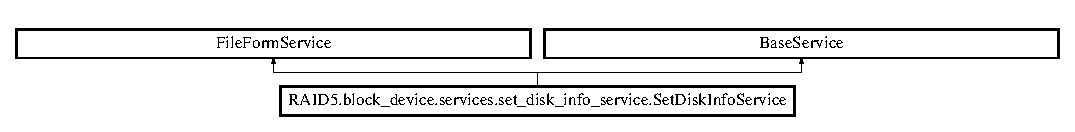
\includegraphics[height=1.320755cm]{class_r_a_i_d5_1_1block__device_1_1services_1_1set__disk__info__service_1_1_set_disk_info_service}
\end{center}
\end{figure}
\subsection*{Public Member Functions}
\begin{DoxyCompactItemize}
\item 
\mbox{\Hypertarget{class_r_a_i_d5_1_1block__device_1_1services_1_1set__disk__info__service_1_1_set_disk_info_service_a475d7ba1551735748b5a226e0113fbd7}\label{class_r_a_i_d5_1_1block__device_1_1services_1_1set__disk__info__service_1_1_set_disk_info_service_a475d7ba1551735748b5a226e0113fbd7}} 
def {\bfseries \+\_\+\+\_\+init\+\_\+\+\_\+} (self, entry, pollables, args)
\item 
\mbox{\Hypertarget{class_r_a_i_d5_1_1block__device_1_1services_1_1set__disk__info__service_1_1_set_disk_info_service_a800282607bae5d6545a1eb4e586ef02c}\label{class_r_a_i_d5_1_1block__device_1_1services_1_1set__disk__info__service_1_1_set_disk_info_service_a800282607bae5d6545a1eb4e586ef02c}} 
def {\bfseries file\+\_\+handle} (self, buf, next\+\_\+state)
\end{DoxyCompactItemize}
\subsection*{Static Public Member Functions}
\begin{DoxyCompactItemize}
\item 
\mbox{\Hypertarget{class_r_a_i_d5_1_1block__device_1_1services_1_1set__disk__info__service_1_1_set_disk_info_service_a72eea80f2a7dea81f2a9b3afcb0e67a2}\label{class_r_a_i_d5_1_1block__device_1_1services_1_1set__disk__info__service_1_1_set_disk_info_service_a72eea80f2a7dea81f2a9b3afcb0e67a2}} 
def {\bfseries get\+\_\+name} ()
\end{DoxyCompactItemize}


The documentation for this class was generated from the following file\+:\begin{DoxyCompactItemize}
\item 
C\+:/cygwin64/tmp/\+R\+A\+I\+D5/block\+\_\+device/services/set\+\_\+disk\+\_\+info\+\_\+service.\+py\end{DoxyCompactItemize}

\hypertarget{classclient_1_1set__block_1_1_start_page}{}\section{client.\+set\+\_\+block.\+Start\+Page Class Reference}
\label{classclient_1_1set__block_1_1_start_page}\index{client.\+set\+\_\+block.\+Start\+Page@{client.\+set\+\_\+block.\+Start\+Page}}
\subsection*{Public Member Functions}
\begin{DoxyCompactItemize}
\item 
\mbox{\Hypertarget{classclient_1_1set__block_1_1_start_page_ad3a0f6a148cc025886a27019b41d7639}\label{classclient_1_1set__block_1_1_start_page_ad3a0f6a148cc025886a27019b41d7639}} 
def {\bfseries \+\_\+\+\_\+init\+\_\+\+\_\+} (self)
\item 
\mbox{\Hypertarget{classclient_1_1set__block_1_1_start_page_aee8f32301a29d5bca44fd782ec14e49c}\label{classclient_1_1set__block_1_1_start_page_aee8f32301a29d5bca44fd782ec14e49c}} 
def {\bfseries run} (self)
\item 
\mbox{\Hypertarget{classclient_1_1set__block_1_1_start_page_a2c3eb3a71a6ca0d78b4622ec6a75be4c}\label{classclient_1_1set__block_1_1_start_page_a2c3eb3a71a6ca0d78b4622ec6a75be4c}} 
def {\bfseries return\+Answer} (self, response)
\end{DoxyCompactItemize}


The documentation for this class was generated from the following file\+:\begin{DoxyCompactItemize}
\item 
C\+:/cygwin64/tmp/\+R\+A\+I\+D5/resources/client/set\+\_\+block.\+py\end{DoxyCompactItemize}

\hypertarget{classstate_1_1_state}{}\section{state.\+State Class Reference}
\label{classstate_1_1_state}\index{state.\+State@{state.\+State}}
Inheritance diagram for state.\+State\+:\begin{figure}[H]
\begin{center}
\leavevmode
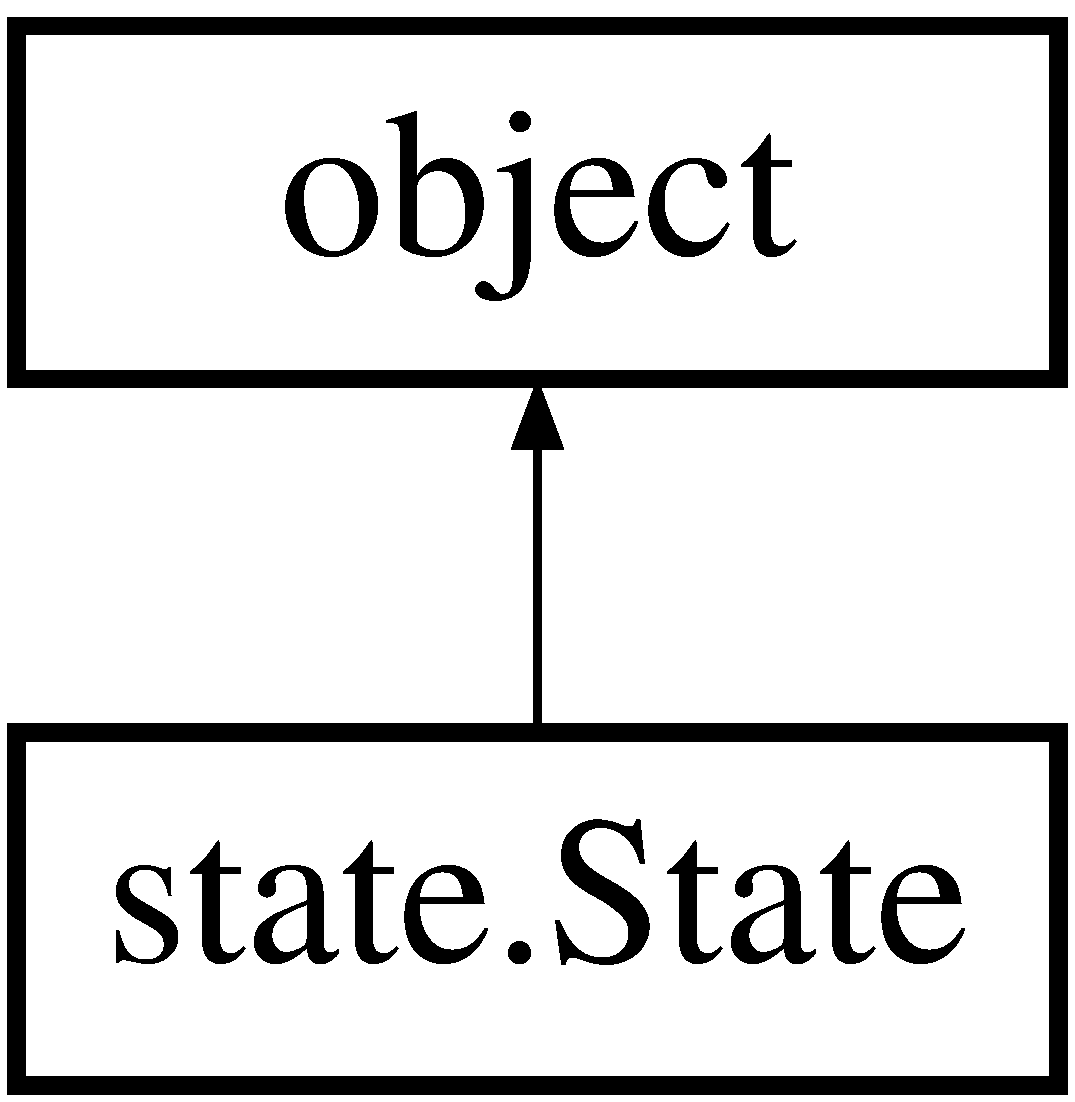
\includegraphics[height=2.000000cm]{classstate_1_1_state}
\end{center}
\end{figure}
\subsection*{Public Member Functions}
\begin{DoxyCompactItemize}
\item 
\mbox{\Hypertarget{classstate_1_1_state_a1223ba69c96efe9b11806a1a7a1c842a}\label{classstate_1_1_state_a1223ba69c96efe9b11806a1a7a1c842a}} 
def {\bfseries default\+\_\+before\+\_\+input\+\_\+func} (self, entry)
\item 
\mbox{\Hypertarget{classstate_1_1_state_ae616a6915ae566c7fb4d0f9ba0bf9898}\label{classstate_1_1_state_ae616a6915ae566c7fb4d0f9ba0bf9898}} 
def {\bfseries default\+\_\+after\+\_\+input\+\_\+func} (self, entry)
\item 
\mbox{\Hypertarget{classstate_1_1_state_aa5a9abc5fbbcba7d22900849175c2802}\label{classstate_1_1_state_aa5a9abc5fbbcba7d22900849175c2802}} 
def {\bfseries \+\_\+\+\_\+init\+\_\+\+\_\+} (self, index, next\+\_\+states, before\+\_\+func=default\+\_\+before\+\_\+input\+\_\+func, after\+\_\+func=default\+\_\+after\+\_\+input\+\_\+func)
\item 
\mbox{\Hypertarget{classstate_1_1_state_a5367de7c27bb7209456b6c0676640c89}\label{classstate_1_1_state_a5367de7c27bb7209456b6c0676640c89}} 
def {\bfseries index} (self)
\item 
\mbox{\Hypertarget{classstate_1_1_state_a849853c72dd3a2f02c05e25b4df2a51d}\label{classstate_1_1_state_a849853c72dd3a2f02c05e25b4df2a51d}} 
def {\bfseries \+\_\+\+\_\+repr\+\_\+\+\_\+} (self)
\item 
\mbox{\Hypertarget{classstate_1_1_state_ad973951b42a2832659ec4d22a164fa2f}\label{classstate_1_1_state_ad973951b42a2832659ec4d22a164fa2f}} 
def {\bfseries before\+\_\+input\+\_\+func} (self)
\item 
\mbox{\Hypertarget{classstate_1_1_state_ad1c54813b9a4ad605443a78f61bedc9e}\label{classstate_1_1_state_ad1c54813b9a4ad605443a78f61bedc9e}} 
def {\bfseries next\+\_\+states} (self)
\item 
\mbox{\Hypertarget{classstate_1_1_state_a39854b37bfe953c78a3ca0d8cd58a723}\label{classstate_1_1_state_a39854b37bfe953c78a3ca0d8cd58a723}} 
def {\bfseries after\+\_\+input\+\_\+func} (self)
\end{DoxyCompactItemize}


The documentation for this class was generated from the following file\+:\begin{DoxyCompactItemize}
\item 
C\+:/cygwin64/tmp/\+R\+A\+I\+D5/frontend/utilities/state\+\_\+util/state.\+py\end{DoxyCompactItemize}

\hypertarget{class_r_a_i_d5_1_1common_1_1utilities_1_1state__util_1_1state_1_1_state}{}\section{R\+A\+I\+D5.\+common.\+utilities.\+state\+\_\+util.\+state.\+State Class Reference}
\label{class_r_a_i_d5_1_1common_1_1utilities_1_1state__util_1_1state_1_1_state}\index{R\+A\+I\+D5.\+common.\+utilities.\+state\+\_\+util.\+state.\+State@{R\+A\+I\+D5.\+common.\+utilities.\+state\+\_\+util.\+state.\+State}}
Inheritance diagram for R\+A\+I\+D5.\+common.\+utilities.\+state\+\_\+util.\+state.\+State\+:\begin{figure}[H]
\begin{center}
\leavevmode
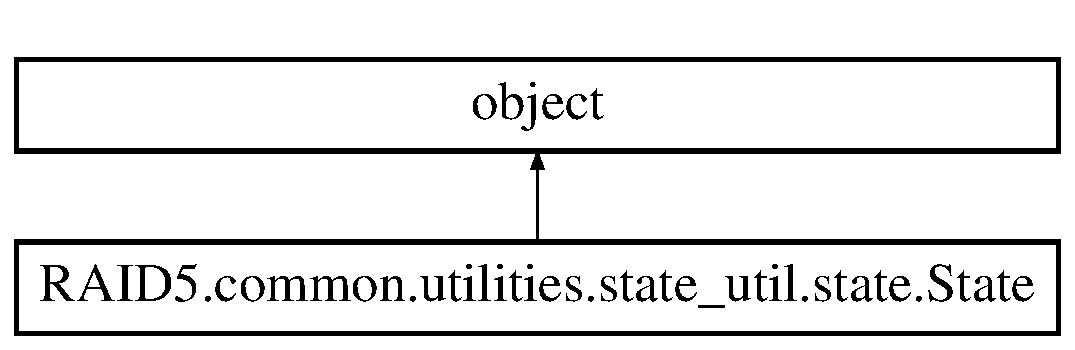
\includegraphics[height=2.000000cm]{class_r_a_i_d5_1_1common_1_1utilities_1_1state__util_1_1state_1_1_state}
\end{center}
\end{figure}
\subsection*{Public Member Functions}
\begin{DoxyCompactItemize}
\item 
\mbox{\Hypertarget{class_r_a_i_d5_1_1common_1_1utilities_1_1state__util_1_1state_1_1_state_ae2d90cae6b850f93d2a7ff49a750fe98}\label{class_r_a_i_d5_1_1common_1_1utilities_1_1state__util_1_1state_1_1_state_ae2d90cae6b850f93d2a7ff49a750fe98}} 
def {\bfseries default\+\_\+before\+\_\+input\+\_\+func} (self, entry)
\item 
\mbox{\Hypertarget{class_r_a_i_d5_1_1common_1_1utilities_1_1state__util_1_1state_1_1_state_aeb87db4b0d21fff38e60de9f8b7125f2}\label{class_r_a_i_d5_1_1common_1_1utilities_1_1state__util_1_1state_1_1_state_aeb87db4b0d21fff38e60de9f8b7125f2}} 
def {\bfseries default\+\_\+after\+\_\+input\+\_\+func} (self, entry)
\item 
\mbox{\Hypertarget{class_r_a_i_d5_1_1common_1_1utilities_1_1state__util_1_1state_1_1_state_a69665cfe04ad740ff2bf1a139ace439b}\label{class_r_a_i_d5_1_1common_1_1utilities_1_1state__util_1_1state_1_1_state_a69665cfe04ad740ff2bf1a139ace439b}} 
def {\bfseries \+\_\+\+\_\+init\+\_\+\+\_\+} (self, index, next\+\_\+states, before\+\_\+func=default\+\_\+before\+\_\+input\+\_\+func, after\+\_\+func=default\+\_\+after\+\_\+input\+\_\+func)
\item 
\mbox{\Hypertarget{class_r_a_i_d5_1_1common_1_1utilities_1_1state__util_1_1state_1_1_state_a94d09a7b55844250d05c6c869eb0e403}\label{class_r_a_i_d5_1_1common_1_1utilities_1_1state__util_1_1state_1_1_state_a94d09a7b55844250d05c6c869eb0e403}} 
def {\bfseries index} (self)
\item 
\mbox{\Hypertarget{class_r_a_i_d5_1_1common_1_1utilities_1_1state__util_1_1state_1_1_state_a3f1a004b30689caf8de7a17c88609d6d}\label{class_r_a_i_d5_1_1common_1_1utilities_1_1state__util_1_1state_1_1_state_a3f1a004b30689caf8de7a17c88609d6d}} 
def {\bfseries \+\_\+\+\_\+repr\+\_\+\+\_\+} (self)
\item 
\mbox{\Hypertarget{class_r_a_i_d5_1_1common_1_1utilities_1_1state__util_1_1state_1_1_state_ae461e9de2a9f8792a3287c5bd3a39eb8}\label{class_r_a_i_d5_1_1common_1_1utilities_1_1state__util_1_1state_1_1_state_ae461e9de2a9f8792a3287c5bd3a39eb8}} 
def {\bfseries before\+\_\+input\+\_\+func} (self)
\item 
\mbox{\Hypertarget{class_r_a_i_d5_1_1common_1_1utilities_1_1state__util_1_1state_1_1_state_ae33babc5dfd98fdc8cb91cd70ad733ba}\label{class_r_a_i_d5_1_1common_1_1utilities_1_1state__util_1_1state_1_1_state_ae33babc5dfd98fdc8cb91cd70ad733ba}} 
def {\bfseries next\+\_\+states} (self)
\item 
\mbox{\Hypertarget{class_r_a_i_d5_1_1common_1_1utilities_1_1state__util_1_1state_1_1_state_a6495efa06f693391c6ebfd9d92607131}\label{class_r_a_i_d5_1_1common_1_1utilities_1_1state__util_1_1state_1_1_state_a6495efa06f693391c6ebfd9d92607131}} 
def {\bfseries after\+\_\+input\+\_\+func} (self)
\end{DoxyCompactItemize}


The documentation for this class was generated from the following file\+:\begin{DoxyCompactItemize}
\item 
C\+:/cygwin64/tmp/\+R\+A\+I\+D5/common/utilities/state\+\_\+util/state.\+py\end{DoxyCompactItemize}

\hypertarget{class_r_a_i_d5_1_1common_1_1utilities_1_1state__util_1_1state__machine_1_1_state_machine}{}\section{R\+A\+I\+D5.\+common.\+utilities.\+state\+\_\+util.\+state\+\_\+machine.\+State\+Machine Class Reference}
\label{class_r_a_i_d5_1_1common_1_1utilities_1_1state__util_1_1state__machine_1_1_state_machine}\index{R\+A\+I\+D5.\+common.\+utilities.\+state\+\_\+util.\+state\+\_\+machine.\+State\+Machine@{R\+A\+I\+D5.\+common.\+utilities.\+state\+\_\+util.\+state\+\_\+machine.\+State\+Machine}}
Inheritance diagram for R\+A\+I\+D5.\+common.\+utilities.\+state\+\_\+util.\+state\+\_\+machine.\+State\+Machine\+:\begin{figure}[H]
\begin{center}
\leavevmode
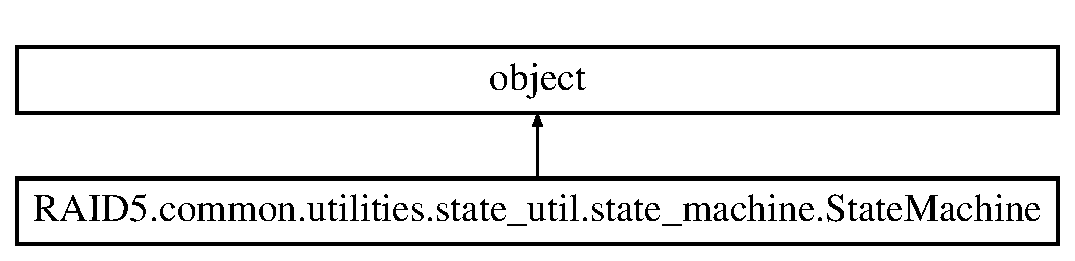
\includegraphics[height=2.000000cm]{class_r_a_i_d5_1_1common_1_1utilities_1_1state__util_1_1state__machine_1_1_state_machine}
\end{center}
\end{figure}
\subsection*{Public Member Functions}
\begin{DoxyCompactItemize}
\item 
\mbox{\Hypertarget{class_r_a_i_d5_1_1common_1_1utilities_1_1state__util_1_1state__machine_1_1_state_machine_afccea2425fb87ba44df1a3adf269db95}\label{class_r_a_i_d5_1_1common_1_1utilities_1_1state__util_1_1state__machine_1_1_state_machine_afccea2425fb87ba44df1a3adf269db95}} 
def {\bfseries \+\_\+\+\_\+init\+\_\+\+\_\+} (self, states, first\+\_\+state, final\+\_\+state)
\item 
\mbox{\Hypertarget{class_r_a_i_d5_1_1common_1_1utilities_1_1state__util_1_1state__machine_1_1_state_machine_afc718a6b19996cb15e81ea6b306e0217}\label{class_r_a_i_d5_1_1common_1_1utilities_1_1state__util_1_1state__machine_1_1_state_machine_afc718a6b19996cb15e81ea6b306e0217}} 
def {\bfseries \+\_\+\+\_\+repr\+\_\+\+\_\+} (self)
\item 
\mbox{\Hypertarget{class_r_a_i_d5_1_1common_1_1utilities_1_1state__util_1_1state__machine_1_1_state_machine_a327d53ef26ad8f41186b1c0ee4fe6985}\label{class_r_a_i_d5_1_1common_1_1utilities_1_1state__util_1_1state__machine_1_1_state_machine_a327d53ef26ad8f41186b1c0ee4fe6985}} 
def {\bfseries run\+\_\+machine} (self, args)
\end{DoxyCompactItemize}


The documentation for this class was generated from the following file\+:\begin{DoxyCompactItemize}
\item 
C\+:/cygwin64/tmp/\+R\+A\+I\+D5/common/utilities/state\+\_\+util/state\+\_\+machine.\+py\end{DoxyCompactItemize}

\hypertarget{classstate__machine_1_1_state_machine}{}\section{state\+\_\+machine.\+State\+Machine Class Reference}
\label{classstate__machine_1_1_state_machine}\index{state\+\_\+machine.\+State\+Machine@{state\+\_\+machine.\+State\+Machine}}
Inheritance diagram for state\+\_\+machine.\+State\+Machine\+:\begin{figure}[H]
\begin{center}
\leavevmode
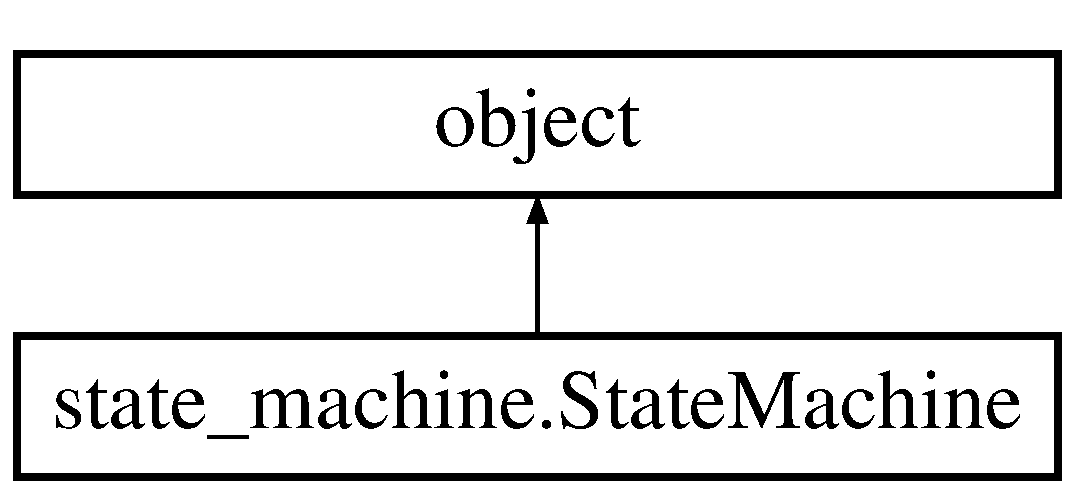
\includegraphics[height=2.000000cm]{classstate__machine_1_1_state_machine}
\end{center}
\end{figure}
\subsection*{Public Member Functions}
\begin{DoxyCompactItemize}
\item 
\mbox{\Hypertarget{classstate__machine_1_1_state_machine_a6dc147a96353e9cdfb91a12e0201eb79}\label{classstate__machine_1_1_state_machine_a6dc147a96353e9cdfb91a12e0201eb79}} 
def {\bfseries \+\_\+\+\_\+init\+\_\+\+\_\+} (self, states, first\+\_\+state, final\+\_\+state)
\item 
\mbox{\Hypertarget{classstate__machine_1_1_state_machine_a6ef1edf09ee6a71495679310a863c58a}\label{classstate__machine_1_1_state_machine_a6ef1edf09ee6a71495679310a863c58a}} 
def {\bfseries \+\_\+\+\_\+repr\+\_\+\+\_\+} (self)
\item 
\mbox{\Hypertarget{classstate__machine_1_1_state_machine_a94a78f44136fa4ed13a02b29d148a095}\label{classstate__machine_1_1_state_machine_a94a78f44136fa4ed13a02b29d148a095}} 
def {\bfseries run\+\_\+machine} (self, args)
\end{DoxyCompactItemize}


The documentation for this class was generated from the following file\+:\begin{DoxyCompactItemize}
\item 
C\+:/cygwin64/tmp/\+R\+A\+I\+D5/frontend/utilities/state\+\_\+util/state\+\_\+machine.\+py\end{DoxyCompactItemize}

\hypertarget{class_r_a_i_d5_1_1frontend_1_1services_1_1time__service_1_1_time_service}{}\section{R\+A\+I\+D5.\+frontend.\+services.\+time\+\_\+service.\+Time\+Service Class Reference}
\label{class_r_a_i_d5_1_1frontend_1_1services_1_1time__service_1_1_time_service}\index{R\+A\+I\+D5.\+frontend.\+services.\+time\+\_\+service.\+Time\+Service@{R\+A\+I\+D5.\+frontend.\+services.\+time\+\_\+service.\+Time\+Service}}
Inheritance diagram for R\+A\+I\+D5.\+frontend.\+services.\+time\+\_\+service.\+Time\+Service\+:\begin{figure}[H]
\begin{center}
\leavevmode
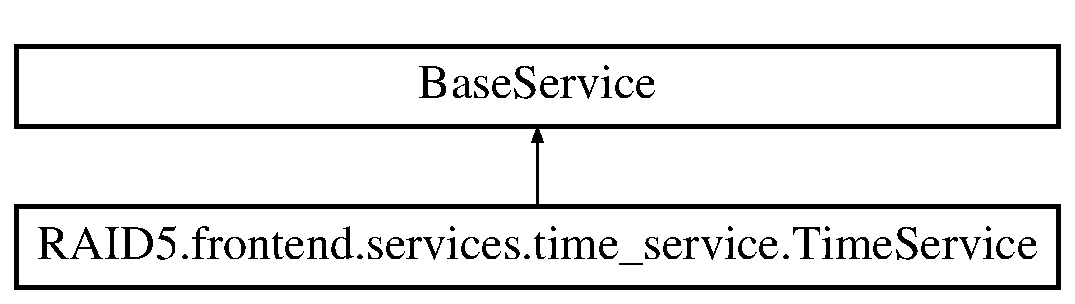
\includegraphics[height=2.000000cm]{class_r_a_i_d5_1_1frontend_1_1services_1_1time__service_1_1_time_service}
\end{center}
\end{figure}
\subsection*{Public Member Functions}
\begin{DoxyCompactItemize}
\item 
\mbox{\Hypertarget{class_r_a_i_d5_1_1frontend_1_1services_1_1time__service_1_1_time_service_a38cf8fb561c015253cc427e640b1e570}\label{class_r_a_i_d5_1_1frontend_1_1services_1_1time__service_1_1_time_service_a38cf8fb561c015253cc427e640b1e570}} 
def {\bfseries \+\_\+\+\_\+init\+\_\+\+\_\+} (self, entry, pollables)
\item 
\mbox{\Hypertarget{class_r_a_i_d5_1_1frontend_1_1services_1_1time__service_1_1_time_service_aff2f55df46713508f13b23b09b0773fe}\label{class_r_a_i_d5_1_1frontend_1_1services_1_1time__service_1_1_time_service_aff2f55df46713508f13b23b09b0773fe}} 
def {\bfseries before\+\_\+response\+\_\+headers} (self, entry)
\end{DoxyCompactItemize}
\subsection*{Static Public Member Functions}
\begin{DoxyCompactItemize}
\item 
\mbox{\Hypertarget{class_r_a_i_d5_1_1frontend_1_1services_1_1time__service_1_1_time_service_a5423d9b5c863fdc89514b9a28b6613a3}\label{class_r_a_i_d5_1_1frontend_1_1services_1_1time__service_1_1_time_service_a5423d9b5c863fdc89514b9a28b6613a3}} 
def {\bfseries get\+\_\+name} ()
\end{DoxyCompactItemize}


The documentation for this class was generated from the following file\+:\begin{DoxyCompactItemize}
\item 
C\+:/cygwin64/tmp/\+R\+A\+I\+D5/frontend/services/time\+\_\+service.\+py\end{DoxyCompactItemize}

\hypertarget{class_r_a_i_d5_1_1block__device_1_1services_1_1update__level__service_1_1_update_level_service}{}\section{R\+A\+I\+D5.\+block\+\_\+device.\+services.\+update\+\_\+level\+\_\+service.\+Update\+Level\+Service Class Reference}
\label{class_r_a_i_d5_1_1block__device_1_1services_1_1update__level__service_1_1_update_level_service}\index{R\+A\+I\+D5.\+block\+\_\+device.\+services.\+update\+\_\+level\+\_\+service.\+Update\+Level\+Service@{R\+A\+I\+D5.\+block\+\_\+device.\+services.\+update\+\_\+level\+\_\+service.\+Update\+Level\+Service}}
Inheritance diagram for R\+A\+I\+D5.\+block\+\_\+device.\+services.\+update\+\_\+level\+\_\+service.\+Update\+Level\+Service\+:\begin{figure}[H]
\begin{center}
\leavevmode
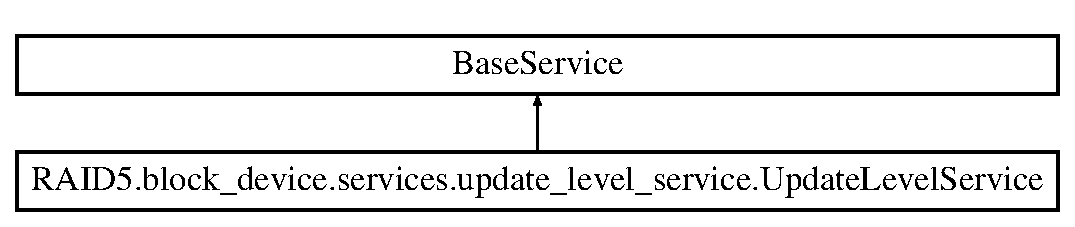
\includegraphics[height=2.000000cm]{class_r_a_i_d5_1_1block__device_1_1services_1_1update__level__service_1_1_update_level_service}
\end{center}
\end{figure}
\subsection*{Public Member Functions}
\begin{DoxyCompactItemize}
\item 
\mbox{\Hypertarget{class_r_a_i_d5_1_1block__device_1_1services_1_1update__level__service_1_1_update_level_service_a09441a50f9cb4c0f0c84918430f60aec}\label{class_r_a_i_d5_1_1block__device_1_1services_1_1update__level__service_1_1_update_level_service_a09441a50f9cb4c0f0c84918430f60aec}} 
def {\bfseries \+\_\+\+\_\+init\+\_\+\+\_\+} (self, entry, pollables, args)
\item 
\mbox{\Hypertarget{class_r_a_i_d5_1_1block__device_1_1services_1_1update__level__service_1_1_update_level_service_a6ce7ce675536e8bb3af37cc1755806a0}\label{class_r_a_i_d5_1_1block__device_1_1services_1_1update__level__service_1_1_update_level_service_a6ce7ce675536e8bb3af37cc1755806a0}} 
def {\bfseries before\+\_\+response\+\_\+status} (self, entry)
\item 
\mbox{\Hypertarget{class_r_a_i_d5_1_1block__device_1_1services_1_1update__level__service_1_1_update_level_service_a95df2438df37413be715f3b846e2a0ec}\label{class_r_a_i_d5_1_1block__device_1_1services_1_1update__level__service_1_1_update_level_service_a95df2438df37413be715f3b846e2a0ec}} 
def {\bfseries before\+\_\+terminate} (self, entry)
\end{DoxyCompactItemize}
\subsection*{Static Public Member Functions}
\begin{DoxyCompactItemize}
\item 
\mbox{\Hypertarget{class_r_a_i_d5_1_1block__device_1_1services_1_1update__level__service_1_1_update_level_service_a3b15a64a007c7091c62be54243ddf44a}\label{class_r_a_i_d5_1_1block__device_1_1services_1_1update__level__service_1_1_update_level_service_a3b15a64a007c7091c62be54243ddf44a}} 
def {\bfseries get\+\_\+name} ()
\end{DoxyCompactItemize}


The documentation for this class was generated from the following file\+:\begin{DoxyCompactItemize}
\item 
C\+:/cygwin64/tmp/\+R\+A\+I\+D5/block\+\_\+device/services/update\+\_\+level\+\_\+service.\+py\end{DoxyCompactItemize}

\hypertarget{class_r_a_i_d5_1_1frontend_1_1services_1_1write__disk__service_1_1_write_to_disk_service}{}\section{R\+A\+I\+D5.\+frontend.\+services.\+write\+\_\+disk\+\_\+service.\+Write\+To\+Disk\+Service Class Reference}
\label{class_r_a_i_d5_1_1frontend_1_1services_1_1write__disk__service_1_1_write_to_disk_service}\index{R\+A\+I\+D5.\+frontend.\+services.\+write\+\_\+disk\+\_\+service.\+Write\+To\+Disk\+Service@{R\+A\+I\+D5.\+frontend.\+services.\+write\+\_\+disk\+\_\+service.\+Write\+To\+Disk\+Service}}
Inheritance diagram for R\+A\+I\+D5.\+frontend.\+services.\+write\+\_\+disk\+\_\+service.\+Write\+To\+Disk\+Service\+:\begin{figure}[H]
\begin{center}
\leavevmode
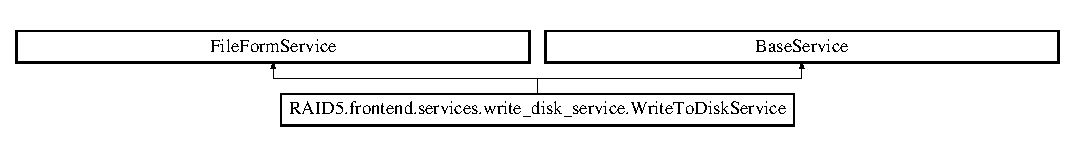
\includegraphics[height=1.462141cm]{class_r_a_i_d5_1_1frontend_1_1services_1_1write__disk__service_1_1_write_to_disk_service}
\end{center}
\end{figure}
\subsection*{Public Member Functions}
\begin{DoxyCompactItemize}
\item 
\mbox{\Hypertarget{class_r_a_i_d5_1_1frontend_1_1services_1_1write__disk__service_1_1_write_to_disk_service_ad57aef29af783bfd059509b460eaa56f}\label{class_r_a_i_d5_1_1frontend_1_1services_1_1write__disk__service_1_1_write_to_disk_service_ad57aef29af783bfd059509b460eaa56f}} 
def {\bfseries \+\_\+\+\_\+init\+\_\+\+\_\+} (self, entry, pollables, args)
\item 
\mbox{\Hypertarget{class_r_a_i_d5_1_1frontend_1_1services_1_1write__disk__service_1_1_write_to_disk_service_aaf701ae764bdfcff7c42542471e3c9f7}\label{class_r_a_i_d5_1_1frontend_1_1services_1_1write__disk__service_1_1_write_to_disk_service_aaf701ae764bdfcff7c42542471e3c9f7}} 
def {\bfseries before\+\_\+content} (self, entry)
\item 
\mbox{\Hypertarget{class_r_a_i_d5_1_1frontend_1_1services_1_1write__disk__service_1_1_write_to_disk_service_ae78ef05dd16f256444f3750d67230032}\label{class_r_a_i_d5_1_1frontend_1_1services_1_1write__disk__service_1_1_write_to_disk_service_ae78ef05dd16f256444f3750d67230032}} 
def {\bfseries arg\+\_\+handle} (self, buf, next\+\_\+state)
\item 
\mbox{\Hypertarget{class_r_a_i_d5_1_1frontend_1_1services_1_1write__disk__service_1_1_write_to_disk_service_afe48bfee7db340690019cf996cbaba2d}\label{class_r_a_i_d5_1_1frontend_1_1services_1_1write__disk__service_1_1_write_to_disk_service_afe48bfee7db340690019cf996cbaba2d}} 
def {\bfseries file\+\_\+handle} (self, buf, next\+\_\+state)
\item 
\mbox{\Hypertarget{class_r_a_i_d5_1_1frontend_1_1services_1_1write__disk__service_1_1_write_to_disk_service_a1844b4f52076c520ef0dc9486476e751}\label{class_r_a_i_d5_1_1frontend_1_1services_1_1write__disk__service_1_1_write_to_disk_service_a1844b4f52076c520ef0dc9486476e751}} 
def {\bfseries on\+\_\+finish} (self, entry)
\item 
\mbox{\Hypertarget{class_r_a_i_d5_1_1frontend_1_1services_1_1write__disk__service_1_1_write_to_disk_service_a5a880601666540590d26f4bf951d64ae}\label{class_r_a_i_d5_1_1frontend_1_1services_1_1write__disk__service_1_1_write_to_disk_service_a5a880601666540590d26f4bf951d64ae}} 
def {\bfseries handle\+\_\+block} (self)
\item 
\mbox{\Hypertarget{class_r_a_i_d5_1_1frontend_1_1services_1_1write__disk__service_1_1_write_to_disk_service_a3174f15c31778680c0f489d75dbaff0a}\label{class_r_a_i_d5_1_1frontend_1_1services_1_1write__disk__service_1_1_write_to_disk_service_a3174f15c31778680c0f489d75dbaff0a}} 
def {\bfseries contexts\+\_\+for\+\_\+reconstruct\+\_\+get\+\_\+block} (self)
\item 
\mbox{\Hypertarget{class_r_a_i_d5_1_1frontend_1_1services_1_1write__disk__service_1_1_write_to_disk_service_ae580905ee78f7c6de6e0ade140263bca}\label{class_r_a_i_d5_1_1frontend_1_1services_1_1write__disk__service_1_1_write_to_disk_service_ae580905ee78f7c6de6e0ade140263bca}} 
def {\bfseries contexts\+\_\+for\+\_\+regular\+\_\+get\+\_\+block} (self)
\item 
\mbox{\Hypertarget{class_r_a_i_d5_1_1frontend_1_1services_1_1write__disk__service_1_1_write_to_disk_service_aee27da3cbe224018b18df3ed0e3c56bf}\label{class_r_a_i_d5_1_1frontend_1_1services_1_1write__disk__service_1_1_write_to_disk_service_aee27da3cbe224018b18df3ed0e3c56bf}} 
def {\bfseries contexts\+\_\+for\+\_\+regular\+\_\+set\+\_\+block} (self)
\item 
\mbox{\Hypertarget{class_r_a_i_d5_1_1frontend_1_1services_1_1write__disk__service_1_1_write_to_disk_service_ae04f93ddddb2b4dbf894d4f7aa73fbdc}\label{class_r_a_i_d5_1_1frontend_1_1services_1_1write__disk__service_1_1_write_to_disk_service_ae04f93ddddb2b4dbf894d4f7aa73fbdc}} 
def {\bfseries contexts\+\_\+for\+\_\+reconstruct\+\_\+set\+\_\+block} (self)
\item 
\mbox{\Hypertarget{class_r_a_i_d5_1_1frontend_1_1services_1_1write__disk__service_1_1_write_to_disk_service_a22d9b97ab2de2bd8f79f9275a9515971}\label{class_r_a_i_d5_1_1frontend_1_1services_1_1write__disk__service_1_1_write_to_disk_service_a22d9b97ab2de2bd8f79f9275a9515971}} 
def {\bfseries create\+\_\+set\+\_\+request\+\_\+info} (self, disk\+\_\+content)
\end{DoxyCompactItemize}
\subsection*{Static Public Member Functions}
\begin{DoxyCompactItemize}
\item 
\mbox{\Hypertarget{class_r_a_i_d5_1_1frontend_1_1services_1_1write__disk__service_1_1_write_to_disk_service_a36546dcbe697f726ee0434d65b2ff8c4}\label{class_r_a_i_d5_1_1frontend_1_1services_1_1write__disk__service_1_1_write_to_disk_service_a36546dcbe697f726ee0434d65b2ff8c4}} 
def {\bfseries get\+\_\+name} ()
\end{DoxyCompactItemize}


The documentation for this class was generated from the following file\+:\begin{DoxyCompactItemize}
\item 
C\+:/cygwin64/tmp/\+R\+A\+I\+D5/frontend/services/write\+\_\+disk\+\_\+service.\+py\end{DoxyCompactItemize}

%--- End generated contents ---

% Index
\backmatter
\newpage
\phantomsection
\clearemptydoublepage
\addcontentsline{toc}{chapter}{Index}
\printindex

\end{document}
